\section{The Complicity Spiral: How to Make Everyone Dirty So No One Can Cleanly Leave}

\vfill


\begin{figure}[H]
  \centering
  
  % === First row ===
  \begin{subfigure}[t]{0.45\textwidth}
  \centering
  \begin{tikzpicture}
    \comicpanel{0}{0}
      {Centauri Exec}
      {Aurora Founder}
      {Tonight’s not about contracts. It’s about belonging.}
      {(-0.6,-0.6)}
  \end{tikzpicture}
  \caption*{The invitation: ambiguous, alluring, loaded.}
  \end{subfigure}
  \hfill
  \begin{subfigure}[t]{0.45\textwidth}
  \centering
  \begin{tikzpicture}
    \comicpanel{0}{0}
      {Centauri Exec}
      {Aurora Founder}
      {Belonging to what?}
      {(0.6,-0.6)}
  \end{tikzpicture}
  \caption*{The hesitation: unease creeping beneath the promise.}
  \end{subfigure}
  
  \vspace{1em}
  
  % === Second row ===
  \begin{subfigure}[t]{0.45\textwidth}
  \centering
  \begin{tikzpicture}
    \comicpanel{0}{0}
      {Centauri Exec}
      {Aurora Founder}
      {The "group". Everyone in that room’s done each other favors. That’s why it works.}
      {(-0.6,-0.6)}
  \end{tikzpicture}
  \caption*{The reassurance: a quiet implication of reciprocity.}
  \end{subfigure}
  \hfill
  \begin{subfigure}[t]{0.45\textwidth}
  \centering
  \begin{tikzpicture}
    \comicpanel{0}{0}
      {Centauri Exec}
      {Aurora Founder}
      {And what if I don’t want to owe anyone favors?}
      {(0.6,-0.6)}
  \end{tikzpicture}
  \caption*{The warning: a question asked too late.}
  \end{subfigure}
  
  \caption*{In some rooms, the price of entry isn’t on the invitation. It’s in the tab you don’t know you’re running.}
\end{figure}



\subsection{The Prologue}

“You said no more of this,” Emma said from the doorway, flipping the hallway switch with a snap. The overhead light 
washed the room in white.

The kitchen had the polished chill of a showroom: quartz counters, brushed steel appliances, a reclaimed wood island 
that still smelled faintly of lemon oil and garlic. The dinner dishes were stacked in the sink, mostly untouched. 
A half-empty bottle of Glenfidick 18 stood like a forgotten prop near the fruit bowl. Above the stove, a digital clock 
glowed 2:11 a.m.

Outside, a thin sheet of snow drifted against the glass door leading to the backyard, where the swing set sat unused. 
Inside, the room was still — not quiet, exactly, but paused, like a breath being held.

David didn’t look up. “It’s just one last push.”

“You said that last week. And the week before.”

“This one’s different. I’m speaking tomorrow. The conference panel—”

“—doesn’t tuck the kids in,” she cut in.

His eyes shifted briefly toward the fridge. Taped near the handle was a photo of the kids in Halloween costumes: a picakachu 
and a care bear. One of them had drawn crooked lightning bolts around the border with a blue marker. He stared at it for a 
moment too long.

She doesn’t understand, he thought. Not really. Not what it means to carry the weight of something invisible. Not what it’s 
like to wake up with ambition burning holes in your gut and go to bed still feeling behind. This wasn’t about ego. It was 
about survival. Legacy. Keeping them safe in a world that didn’t care.

He sat at the island, still in his t-shirt from the day before. The light from his laptop screen cast pale-blue shadows 
across the counter. Slide 14 was on the screen again: \textit{Risk Stratification Under Uncertainty}. He adjusted a 
y-axis, then stared at it like it owed him something.

Emma walked to the fridge, opened it, and just stood there, unmoving. A bottle of wine shifted slightly but she let it 
settle. The soft whir of the appliance filled the silence between them.

“You promised this would be better,” she said. “That starting your own business meant more time for us. Not... 
whatever this is.”

He sighed. “You know this is for us, right? The whole point is—”

“You’re pitching to your wife at two in the morning. Do you hear yourself?”

He finally turned. “I’m trying to build something that lasts.”

Emma leaned on the counter, arms crossed. “What if we already have something that lasts, and you’re too busy optimizing 
it into oblivion?”

He didn’t answer. She glanced at the screen.

“Let me guess. Twenty-five slides, and zero about what it’s costing you.”

“It’s costing us now so it doesn’t later.”

She looked at him the way someone looks at a person they love when they suspect the real goodbye already 
happened months ago.

“Just... don’t sell your soul.”

David smiled, the kind of smile that knew too much and said too little. “I would never do that. I’m doing this for us.”

She didn’t argue. That was the part that landed harder.

“That’s what makes it scarier,” she said, and walked away.

The sound of her slippers faded down the hall, muffled but final. The house seemed colder without her in the room. 
David sat there, unmoving.

Then, quietly, he deleted the phrase \textit{“adaptive resilience”} and typed:

\textbf{Compliant AI Infrastructure for Enterprise Risk.}

He stared at it.

Then clicked save.


\medskip

\begin{PsychologicalSidebar}{The Builder’s Paradox}

  David isn’t selfish. He’s committed.

  \medskip
  
  That’s what makes it dangerous.
  
  \medskip
  
  In Cognitive Behavioral Therapy (CBT), there’s a class of mental traps called \textbf{cognitive distortions}: 
  patterns of thought that feel rational, but quietly sabotage well-being.

  \medskip
  
  David’s internal script checks multiple boxes:

  \medskip
  
  \begin{itemize}
    \item \textbf{All-or-Nothing Thinking:} “If I don’t make this work, I’ve failed my family.”
    \item \textbf{Fortune Telling:} “Once this deal closes, things will calm down.”
    \item \textbf{Emotional Reasoning:} “I feel guilty when I rest; therefore, I must not deserve to rest.”
  \end{itemize}
  
  \medskip
  
  These distortions feed into a larger psychological dynamic:  
  \textbf{goal substitution}. This happens when a person replaces a real goal (family, connection, presence) 
  with a symbolic one (success, income, prestige) because the latter is easier to measure and harder to challenge.

  \medskip
  
  Over time, the means becomes the mission.  
  The system becomes self-justifying.  
  And the more sacrifice he makes, the more he feels obligated to make it worth something: a classic \textbf{sunk cost fallacy}.
  
  \medskip
  
  That’s why Emma’s words don’t break through.  
  David’s not ignoring her. He’s defending a narrative that keeps him going.
  
  \medskip
  
  So when he hits “save,” he’s not just preserving a PowerPoint.
  He’s reaffirming a distortion.  
  And crossing a line he doesn’t fully see... yet.
  
\end{PsychologicalSidebar}

\subsection{Editor Questions for ``The Prologue''}

To get meaningful and diverse feedback, I designed these questions to go beyond surface-level edits. 
I need you to reflect not just on technical clarity or style, but on emotional resonance, character 
believability, narrative structure, pacing, and thematic depth. You don’t need to answer every question. 
Please focus on the ones that speak to your experience as a reader. The goal is not to fix the scene, but 
to understand how it lands, where it connects, and where it might quietly miss.


\subsubsection{Narrative \& Structure}

\begin{itemize}
  \item Did this feel like the right way to open the story? Why or why not?
  \item Was the pacing effective? Did it hold your attention throughout the scene?
  \item Did anything feel redundant or like it could be trimmed without losing impact?
\end{itemize}

\subsubsection{Emotional Resonance}

\begin{itemize}
  \item How did this scene make you feel? Were you more aligned with David, Emma, or torn?
  \item Did Emma’s final line (“That’s what makes it scarier”) land for you emotionally? Why or why not?
  \item Was there a moment where you really felt the tension — or where it broke?
\end{itemize}

\subsubsection{Character Insight}

\begin{itemize}
  \item Did David feel like a real person to you? Did his motivations make sense?
  \item Did Emma’s dialogue and reactions feel grounded and believable?
  \item What assumptions do you find yourself making about their relationship based on this scene?
\end{itemize}

\subsubsection{Psychological Sidebar}

\begin{itemize}
  \item Did the psychological sidebar enhance your understanding of David? Or did it feel like too much explanation?
  \item Would you prefer the sidebar be integrated into the narrative or kept separate like this?
  \item Was anything in the sidebar particularly insightful or redundant?
\end{itemize}

\subsubsection{Theme \& Message}

\begin{itemize}
  \item What do you think this scene is ultimately about?
  \item Did it raise any personal or philosophical questions for you?
  \item Do you feel like this is “just a marriage scene,” or something larger about ambition, modern work, or identity?
\end{itemize}

\subsubsection{Style \& Craft}

\begin{itemize}
  \item Was there a line or image that stuck with you — positively or negatively?
  \item Did the rhythm of the dialogue feel natural?
  \item Did you notice any clichés or overused tropes that undercut the scene’s originality?
\end{itemize}

\subsubsection{Optional: Deeper Testing}

\begin{itemize}
  \item How would your impression of David change if the sidebar wasn’t included?
  \item If you had to cut 20\% of this section, what would go?
  \item If you read this cold — with no context — what genre or tone would you expect the rest of the story to take?
\end{itemize}


\subsection{The Conference}

Michael Hart was in the audience.

Technically, he wasn’t supposed to be at the conference. A client meeting had fallen through, and instead 
of flying out early, he decided to walk the floor. Kill a day. Stay curious. The kind of curiosity 
that made money.

The conference center was all beige carpet, branded lanyards, and tepid coffee in compostable cups. Rows of 
LED-lit booths advertised “responsible AI,” “quantified resilience,” and “next-gen compliance intelligence.” 
One corner featured a sponsored espresso bar. Another had massage chairs under a banner that read: 
\textit{“De-risk your week.”}

Hart didn’t blend in. Not just because of the Tom Ford suit or the black-on-black oxford shoes. It was the 
way he moved: not networking, but hunting. While others nodded through panels with the slack-jawed politeness 
of jetlagged consultants, Hart listened.

Really listened.

He sat two rows from the front. Elbows on knees. Eyes narrowed slightly. And by the second case study, he knew.

This wasn’t just another founder spinning buzzwords. David had edge. The kind that didn’t come from pitch decks. 
The kind that came from bloodied prototypes and quiet bets placed at 2 a.m.

After the panel, while others queued for coffee or badge scans, Hart moved straight toward the stage. No small talk. 
No handshake.

“I’ve got distribution,” he said. “You’ve got product.”

He handed David a business card. White. Unembossed. Just a name, number, and a discreet logo in matte black.

“Let’s talk.”

Then he walked away — the kind of exit that didn’t invite follow-up.

Hart was the founder of Centauri Consulting, which billed itself as “the velvet glove of high-stakes transformation.” 
He didn’t just sell strategic roadmaps. He sold access. His firm specialized in landing contracts other firms 
couldn’t even bid for: the kind where success wasn’t measured in deliverables, but in who picked up the phone.

Centauri didn’t advertise. It didn’t recruit on LinkedIn. It wasn’t looking for clients.

It was looking for \textbf{technical talent it couldn’t poach outright}.


\medskip

\begin{HistoricalSidebar}{The Dark Side of Acquihires --- When Talent Becomes Leverage}

  In the early 2000s, as Silicon Valley’s war for engineering talent reached fever pitch, a new acquisition model 
  quietly took over the startup ecosystem: the \textbf{acquihire}.

  \medskip
  
  Unlike a traditional acquisition, where the buyer wants the product, patents, or market share, an acquihire’s primary 
  target is \textbf{the team}. The startup itself might be shut down, its technology shelved, its users abandoned. The 
  engineers were the real asset.

  \medskip
  
  At first, acquihires were framed as \textit{soft landings} for struggling startups—a face-saving way to pay back 
  investors, a lifeboat for founders, a pathway into Big Tech.

  \medskip
  
  But beneath the glossy press releases, a harsher reality unfolded.

  \medskip
  
  Founders often found themselves negotiating from a position of desperation, their options underwater, their runway gone. 
  Investors pressured them to “return something” rather than risk a total wipeout. Engineers were given golden handcuffs: 
  lucrative retention bonuses tied to multi-year employment agreements, conditional on project milestones that conveniently 
  reset their vesting clocks.

  \medskip
  
  In some cases, acquihires functioned as \textbf{talent raids disguised as mergers}. A competitor could eliminate a rival’s 
  core team while burying its roadmap. A corporation could sidestep a hiring freeze by acquiring headcount off the books.

  \medskip
  
  And for founders, the acquihire wasn’t always an exit—it was a quiet exile.
  
  \medskip
  
  The deeper lesson?

  \medskip
  
  An acquihire doesn’t just buy talent. It \textbf{absorbs leverage}. It converts independent actors into vested stakeholders, 
  ties reputations to institutional outcomes, and rewrites incentives through retention clauses and non-compete agreements.
  Because The real deal isn’t written in the press release.  The real deal is written in the clauses that keep you from leaving.
  
\end{HistoricalSidebar}

\subsection{Editor Questions for ``The Conference''}

To get meaningful and diverse feedback, I designed these questions to go beyond surface-level edits.  
This section isn’t just about whether the scene “works.” It’s about how it lands. Please reflect on the 
emotional tone, narrative economy, character dynamics, and how the themes surface (or don’t). You don’t 
need to answer everything. Focus on what resonates, feels off, or stays with you.

\subsubsection{Narrative \& Structure}

\begin{itemize}
  \item Did this scene flow logically from the previous one? Did the shift in setting feel earned?
  \item Did Hart’s entrance and dialogue create intrigue or momentum?
  \item Was the transition from panel to confrontation clear and compelling?
\end{itemize}

\subsubsection{Character Dynamics}

\begin{itemize}
  \item What do you make of Hart as a character based on this introduction? Did he feel sharp, manipulative, authentic?
  \item Does David’s reaction (or lack of one) tell you anything important?
  \item Did the balance between exposition (e.g., who Centauri is) and action feel natural?
\end{itemize}

\subsubsection{Exposition \& Worldbuilding}

\begin{itemize}
  \item Did you get a clear sense of what Centauri does without it feeling like a pitch?
  \item Were the phrases like “velvet glove of high-stakes transformation” effective or distracting?
  \item Did the exposition about Centauri deepen your understanding of the world or slow things down?
\end{itemize}

\subsubsection{Historical Sidebar}

\begin{itemize}
  \item Did the sidebar on acquihires add context or interrupt the flow?
  \item Was there anything particularly surprising or insightful in the sidebar?
  \item Would you prefer this content embedded in the main narrative, or does the sidebar format work?
\end{itemize}

\subsubsection{Theme \& Message}

\begin{itemize}
  \item What themes do you think are emerging here — power, leverage, co-optation?
  \item Does this scene raise any questions for you about ambition, loyalty, or institutional power?
  \item What tone does this set for the relationship between David and Hart — mentor, opportunist, recruiter?
\end{itemize}

\subsubsection{Style \& Craft}

\begin{itemize}
  \item Was there a sentence or image in this section that stood out to you — positively or negatively?
  \item Did the balance between summary and scene feel right?
  \item Did any part feel overwritten, unclear, or too “corporate”?
\end{itemize}

\subsubsection{Optional: Deeper Testing}

\begin{itemize}
  \item If the Historical Sidebar were cut, what would be lost?
  \item If you didn’t already know David from the previous scene, would this give you a clear sense of who he is?
  \item What do you think Hart’s real agenda is? Did the scene tip its hand too much or too little?
\end{itemize}


\subsection{The Conversation}

They met in the quiet lounge just off the mezzanine — a space meant more for donor schmoozing than deal-making. 
Velvet chairs. Filtered light. A silent espresso machine in the corner that looked sculptural but hissed like a 
snake when used. Someone had left a linen napkin folded on a side table, lipstick print still visible.

Hart didn’t waste time.

“I’ve seen pitch decks with less clarity than your case study,” he said, settling into the chair opposite David 
without removing his coat.

David nodded, cautious. The coffee in his hand was mostly cold. He wasn’t used to being approached like this — 
not directly, not without pretext.

“You built that yourself?” Hart asked.

“Yeah,” David said. “Most of it.”

“What’s your background?”

“Quant. I used to build pricing models at a high-frequency shop.”  
He hesitated. “We blew up during the COVID carry unwind. No fraud. Just… leverage and luck.”

Hart raised an eyebrow. “So instead of finding another job, you decided to build one.”

David half-smiled. “Something like that.”

He explained the idea: a compliance tool — built with the precision of trading infrastructure — that could automate 
the data due diligence financial regulators required.  
Not just a checklist. A framework. Something that could scan model documentation, track revision histories, flag 
missing disclosures, and render it all into audit-grade reports — no team of analysts required.

Hart sat forward. His gaze sharpened.

“You’re not building regtech,” he said. “You’re building capacity.”

David looked puzzled.

Hart clarified: “You’re not replacing a process. You’re replacing a personnel problem.”

He laid it out plainly. Most mid-tier hedge funds were boxed in.  
They didn’t have the budget to hire elite ML compliance engineers. That talent went straight to Goldman, Citadel, 
or was padded behind big-tech RSUs. The rest? Hard to find. Harder to keep.

“If you can get those shops to 80\% compliant without hiring a team to maintain the stack,” Hart said, “you’re not 
just solving a problem. You’re leveling the field.”

David said nothing. The hum of the nearby HVAC unit filled the pause.

Hart didn’t mind the silence. He leaned back just slightly, as if to signal: you’re the one being interviewed now.

“You won’t make them Goldman,” he said. “But you’ll lower the barrier to entry. That’s enough. That’s how markets shift.”

Then, softer, more pointed:

“You don’t need my validation. You’ve got product. What you need is volume.”

He tapped the card he’d laid on the table.

``I know who needs this. Let’s talk.''

\medskip

\begin{HistoricalSidebar}{The Anatomy of a Value Proposition: Why Some Products Land and Others Stall}

  A \textbf{value proposition} is not what a product \textit{does} — it's what it \textbf{solves}. And in markets 
  crowded with technical talent and noise, clarity about that distinction can determine whether a startup takes 
  off or disappears.
  
  \medskip
  
  In startup mythology, product-market fit often gets all the attention. But what gets overlooked is \textbf{problem-founder fit}: 
  whether the founder truly understands the pain they’re solving — and who has it.
  
  \medskip
  
  \textbf{Successful Example: Stripe (2010)}  
  Most payment platforms in 2010 focused on buyers. Stripe targeted \textit{developers} — the engineers tasked with integrating 
  payment APIs. Their value proposition wasn’t “payments made easy,” it was:  
  \textit{“You can deploy a full payments stack in 7 lines of code.”}  
  The problem wasn’t payments — it was \textbf{friction}. Stripe solved for the person who had to ship working code by the end 
  of the week.
  
  \medskip
  
  \textbf{Failed Example: Color Labs (2011)}  
  Color Labs raised \$41 million to launch a social photo app that let users share images with people nearby. The technology 
  was novel — using GPS and proximity to build social networks on the fly — but the value proposition was fuzzy:  
  \textit{“Take pictures together in real-time.”}  
  What problem did it solve? Who needed it? Why now? Users didn’t know. Neither did investors by the time it folded.
  
  \medskip
  
  \textbf{Gray Zone Example: Juicero (2013)}  
  Juicero’s product — a \$400 cold-press juicer — was marketed as a health-tech device with subscription-based juice packets. 
  On paper, it sounded modern and slick. But once people realized you could squeeze the packets by hand, the core value 
  proposition evaporated:  
  \textit{It wasn't about juice. It was about perceived luxury.}  
  The mismatch between actual utility and projected status killed the brand.
  
  \medskip
  
  \textbf{The lesson?}  
  Value proposition design isn’t about feature lists — it’s about mapping your product to a very specific bottleneck in someone 
  else’s world. The sharper the bottleneck, the clearer the value.
  
  \medskip
  
  That’s why Hart zeroed in on David’s tool. Not because it was novel, but because it solved a specific institutional constraint:  
  \textit{“Get to 80\% compliance without hiring.”}
  
\end{HistoricalSidebar}



The second pour of scotch had softened the edges.

They were seated in the lounge of the downtown private club — all brushed brass and low lighting, the kind of place 
designed to look expensive without feeling new. Outside, the city buzzed with Thursday night urgency, but inside, 
everything moved slower. Intentional. The table was marble, veined with gold, chilled to the touch. The waiter had 
long since faded into the background.

The pitch was over. Now came the calculus.

Hart leaned in, elbows on the stone.

“You’re not building a compliance product,” he said. “You’re building a *keycard*.”

David blinked once, slowly. “Keycard?”

Hart didn’t smile. He clarified without condescension:

“You’re not solving for oversight. You’re solving for access. You’re handing mid-tier funds a way into a market they were 
never allowed to touch.”

On the other side of the table, Penn looked up from the term sheet he’d been annotating with a silver Montblanc. He didn’t 
interrupt. Just listened.

Hart continued:

“High-frequency trading isn’t locked off because of regulation. It’s locked off because of *stack complexity*. 
Infrastructure. Latency. State handling. Data streaming. And yeah, regulatory overlays — but those come after.”

David nodded slowly, his fingers wrapped around the base of his glass. “Most of them don’t even try. The bar’s too high.”

“Exactly,” Hart said. “They’re priced out by the engineering curve. Not the compliance curve. You flatten that curve, you 
open the gate.”

The ice in David’s glass cracked gently, like it had been waiting for the moment.


\medskip

\begin{TechnicalSidebar}{Barriers to Entry and Why Most Funds Stay Out}

  A \textbf{barrier to entry} is anything that prevents a new player from entering a market and competing effectively.  
  These barriers aren’t always regulatory. In fintech and high-frequency trading (HFT), they’re often 
  \textit{technical, infrastructural, or cultural}.
  
  \medskip
  
  \textbf{In HFT and ML-driven trading, the primary barriers include:}

  \medskip
  
  \begin{itemize}
    \item \textbf{Stack Complexity:}  
    Millisecond-level latency requirements, real-time introspection, and fault-tolerant event handling pipelines.
  
    \item \textbf{Talent Scarcity:}  
    Engineers who understand trading systems, compliance hooks, and low-level performance tuning are rare — and expensive.
  
    \item \textbf{Regulatory Overlay:}  
    Once infrastructure exists, it must also meet legal standards — audit logs, fair execution, capital disclosures — without slowing performance.
  
    \item \textbf{Reputational Signaling:}  
    Even with a working stack, institutional allocators are wary of unknown platforms without validation from top-tier logos.
  \end{itemize}
  
  \medskip
  
  \textbf{The Result?}  
  Even well-capitalized funds avoid building from scratch.  
  Not because they don’t want to — but because the path to parity is too steep, too slow, and too expensive.
  
  \medskip
  
  \textbf{The strategic unlock?}  
  Build a system that \textit{collapses the engineering barrier} without compromising regulatory posture.  
  Suddenly, you’re not selling software. You’re selling \textbf{access}.
  
\end{TechnicalSidebar}


\medskip

The scotch had mellowed, but the air stayed sharp — not from conflict, but from the clarity that only comes when no one’s 
pretending anymore. The room had the lacquered hush of old money: recessed lights, no music, and walls lined with abstract 
art chosen more for tax deduction than taste.

Outside, the city blurred under halogen and mist, but in here, everything had slowed to a crisp, analytical tempo.

David described the pipeline again — not as a product, but as a vertical-integration play:  
an internal model engine, backtesting under stress scenarios, pipeline introspection, and compliance hooks all rendered 
into modular, containerized deploys.

“You don’t build a product,” Hart said. “You build entry velocity.”

David raised an eyebrow. “Meaning?”

Hart smiled faintly, resting his glass on the marble.

“Meaning they can go from zero to trading without hiring Citadel’s shadow stack.”

Penn folded the term sheet and tapped the cover with two fingers, like sealing an envelope.

“So you’re not selling features. You’re selling qualification.”

“Exactly,” Hart replied. “Most people fail the entry exam. You let them cheat.”

Hart pivoted, now sketching the business model in the air with his hand.

“You don’t price it like a SaaS tool. You price it like a futures contract.  
You’re not charging for usage. You’re charging for entry rights.”

David stayed silent. This wasn’t how he had framed it — but it clicked.  
Not a toolkit. Not a reg layer.

A gateway.

And gateways? Those get priced by what they unlock.




The bar was dim, upscale but unpretentious --- the kind of place where the lighting was low enough to suggest intimacy, 
but not so low that you couldn’t read a term sheet. A jazz trio murmured in the corner, and the leather booths smelled 
faintly of cedar and citrus polish.

Hart pulled a cocktail napkin toward him and clicked a pen from his jacket. He didn’t bother asking for a fresh sheet of paper.

\textit{``Let’s run the numbers,''} he said, scribbling a row of assumptions down the margin. \textit{``Not investor math. 
Fermi math.''}

Morales grinned and leaned in. \textit{``Back-of-the-envelope?''}

\textit{``Always,''} Hart said. \textit{``It’s not about precision. It’s about order of magnitude sanity.''}

He drew three columns: headcount, compliance burden, deployment velocity.

\textit{``Say a fund with \$300 million AUM wants to scale into synthetic credit. Normally they’d need---what---five headcount 
just to maintain reporting compliance?''}

\textit{``Minimum,''} David said. \textit{``Assuming no turnover.''}

\textit{``Right,''} Hart said, underlining the number. \textit{``Now suppose your pipeline replaces three of those roles 
and reduces latency by 60\%. What does that buy them?''}

\textit{``Speed to market. And internal optics.''}

Hart nodded. \textit{``And optics translate into allocation. Faster compliance means faster scaling.''}

He tapped the napkin, now smudged with numbers and ink streaks.

\textit{``That’s your margin,''} he said. \textit{``Not in features. In time arbitrage.''}

David stared at the scribbled napkin. The math was loose. But the logic was airtight.

He didn’t need a calculator. He needed a clock.

And Hart had just reset it.

\medskip


\begin{HistoricalSidebar}{Fermi Estimation: How Atomic Physics Became a Quant Interview Question}

  In July 1945, at the Trinity nuclear test site in New Mexico, Enrico Fermi stood among a group of physicists waiting for 
  history to unfold.  
  As the countdown to the first atomic explosion reached zero, Fermi performed an odd, almost casual act: he dropped small 
  scraps of paper.
  
  \medskip
  
  When the shockwave from the detonation reached him, he observed how far the papers had traveled.  
  From that simple displacement, he estimated the blast yield at approximately 10 kilotons of TNT.
  
  \medskip
  
  Official measurements later put it at about 18.6 kilotons — meaning Fermi, with no instruments and only a handful of confetti, 
  was within a factor of 2.
  
  \medskip
  
  This moment became legend: not because of the accuracy, but because of the method.  
  Fermi didn’t measure. He decomposed the problem into approximate parts — what we now call a \textbf{Fermi estimate}.
  
  \medskip
  
  \textbf{Fermi estimation} is a mental technique for approximating a quantity using only logical reasoning and 
  order-of-magnitude assumptions.  
  It’s the art of going from ``I have no idea'' to ``I have a rough sense'' using structured guesswork.
  
  \medskip
  
  \textbf{The canonical example:}  
  \textit{How many piano tuners are there in Chicago?}

  \medskip
  
  \begin{itemize}
    \item Population of Chicago: \textasciitilde3 million  
    \item Average household size: 2.5 $\Rightarrow$ 1.2 million households  
    \item Households with pianos: \textasciitilde1 in 20 $\Rightarrow$ 60,000 pianos  
    \item Tunings per piano per year: 1  
    \item Total tunings: 60,000/year  
    \item A tuner can do 4 jobs/day, 5 days/week, 50 weeks/year = 1,000 tunings/year  
    \item Needed tuners: 60,000 / 1,000 = \textbf{60 piano tuners}
  \end{itemize}
  
  \medskip
  
  Of course, the real number might be 50 or 80. But that’s not the point.  
  What matters is the \textbf{reasoning}.
  
  \medskip
  
  That’s why Fermi questions became a staple of quant interviews, startup pitches, and market strategy sessions.  
  They don’t test precision.  
  They test \textbf{decomposition, intuition, and the courage to guess}.
  
  \begin{quote}
  \textit{“All models are wrong,”} the saying goes, \textit{“but some are useful.”}  
  Fermi estimates live in that exact margin.
  \end{quote}
  
  \medskip
  
  Whether estimating nuclear yields or billion-dollar TAMs, Fermi logic reminds us:  
  You don’t need perfect data to make a high-quality decision.  
  You just need the guts to bound the problem — and the clarity to own your assumptions.
  
\end{HistoricalSidebar}
  



The napkin was already cluttered, but Hart kept writing.

\textit{``There are about 5{,}000 hedge funds globally,''} he said, thinking aloud. \textit{``Call it 2{,}000 
that are small-to-mid tier — the kind that can’t build their own infra stack.''}

David leaned over the table.

\textit{``Assume 5\% are actively trying to expand into ML-based quant. That’s 100 funds.  
We could reasonably sell to half over five years if we build a reputation. So 50 logos?''}

Hart nodded.

\textit{``Call it 10 the first year. If they pay \$250{,}000 each, that’s \$2.5 million topline.  
Think pilot licenses, integration, and support.''}

David sipped his drink. \textit{``And that’s before we license the IP or run API-based usage tiers.''}

\textit{``Exactly,''} Hart said. \textit{``If even 20\% of the target market scales usage and upgrades to \$500{,}000 per year,  
we’re looking at \$10–15 million annual run rate within 3 years.''}

David tapped the napkin.

\textit{``So you frame it like this:''}

\begin{itemize}
  \item 2{,}000 mid-tier funds  
  \item 5\% are likely early adopters  
  \item Conservative 50-client penetration over 5 years  
  \item \$250{,}000–\$500{,}000 per client
\end{itemize}

Hart leaned back, smiling.

\textit{``Exactly. Market isn’t huge. But it’s deep. It's high trust, high margin, and high retention.  
And once the first five logos land, the rest follow.  
Because nobody wants to be the last quant fund without a real-time audit layer.''}

David nodded slowly.

\textit{``And if you wrap the IP into a licensing structure, the revenue multiple goes from 5x to 12x overnight.  
TAM is maybe \$500 million globally. We don’t need it all. We just need the perception that we could take 10\%.''}

Hart smirked.

\textit{``And that’s how you Fermi your way into a \$50 million valuation in the first year after deployment.''}


\medskip

\begin{TechnicalSidebar}{Business Viability, Payback Period, and Why VCs Care About Speed}

  One of the most underrated metrics in early-stage venture capital isn’t TAM, burn rate, or even ARR.  
  It’s \textbf{payback period} — the time it takes for a new customer to generate enough revenue to cover their own acquisition cost.
  
  \medskip
  
  \textbf{Payback Period Formula:}
  \[
  \text{Payback Period} = \frac{\text{Customer Acquisition Cost (CAC)}}{\text{Gross Margin from Customer per Month}}
  \]
  
  \medskip
  
  If it costs \$50,000 to close a deal and that customer brings in \$25,000 per month in margin,  
  the payback period is 2 months.
  
  \medskip
  
  \textbf{Why it matters:}
  
  \begin{itemize}
    \item Short payback = fast reinvestment cycles. A startup can recycle revenue into more growth without needing new funding.
    \item Long payback = higher risk. The startup must float costs for months (or years) before breakeven.
    \item For VC firms, short payback implies \textbf{capital efficiency} — every dollar deployed drives quicker returns.
  \end{itemize}
  
  \medskip
  
  In the case of Hart and Morales’ strategy:

  \medskip
  
  \begin{itemize}
    \item Each client pays \$250K to \$500K annually.
    \item The product is deployed quickly — modular, containerized, low-integration overhead.
    \item Gross margins exceed 80\%, given the IP-heavy, low-support model.
  \end{itemize}
  
  \medskip
  
  Even assuming \$50K to acquire each customer, they break even within 3 months.  
  That puts them in elite territory — where CAC is recouped before the second quarter, and LTV/CAC ratios can exceed 8x.
  
  \medskip
  
  \textbf{The VC view:}  
  This isn’t just a niche tool. It’s a high-trust, high-ticket product with low churn and fast returns.
  
  \begin{quote}
  \textit{In venture math, velocity beats volume.  
  A product that pays itself back in 90 days can be scaled   
  (even before it's perfect).}
  \end{quote}
  
\end{TechnicalSidebar}
  

\medskip



Hart was drawing boxes on the napkin again.

\textit{``Let’s scale this. Think beyond hedge funds. Who else needs this?''}

David didn’t hesitate.

\textit{``Anyone algorithmically allocating capital under regulatory pressure:''}

\begin{itemize}
  \item Banks with quant desks  
  \item Sovereign wealth arms  
  \item Insurance and pensions migrating into automated trading  
  \item Even crypto funds trying to look institution-grade
\end{itemize}

Hart tapped his pen twice. \textit{``So what’s the real market size?''}

David ran the numbers aloud.

\textit{``Globally? Maybe 30{,}000 institutional allocators.  
Say 10{,}000 are actively integrating ML or automation over the next five years.  
Conservatively, 20\% are in position to buy infra — that’s 2{,}000 serious prospects.''}

Hart grinned. \textit{``Then we blitz it.''}

David raised an eyebrow. \textit{``You’re saying go wide before we even optimize?''}

\textit{``Exactly,''} Hart replied. \textit{``Control’s a second-mover problem.  
Right now, we’re building surface area. \$500K/year base. \$1 million-plus for full access: audit layer, 
traceability, and IP hooks.  
You don’t trickle this in. You carpet-bomb the category. Own the narrative before anyone else knows 
there’s a war.''}

David scratched numbers into the corner of the napkin.

\textit{``Mid-curve case:''}

\begin{itemize}
  \item 1{,}000 clients in 6 years  
  \item Average \$750K/year  
  \item \$750M ARR potential
\end{itemize}


\medskip

\begin{TechnicalSidebar}{What is ARR and Why Does It Matter?}

  \textbf{ARR}, or \textit{Annual Recurring Revenue}, is a core metric for evaluating the health and scalability of 
  a subscription-based business.  
  It answers one question: \textbf{If we changed nothing, how much revenue would we make next year?}
  
  \medskip
  
  Unlike one-time sales or services, ARR assumes continuity — customers staying onboard, renewals flowing in, and 
  contracts holding steady.  
  This makes it a preferred benchmark for investors, especially in enterprise SaaS, infrastructure, and 
  fintech platforms.
  
  \medskip
  
  \textbf{Why do investors care?}

  \medskip
  
  \begin{itemize}
    \item \textbf{Predictability:} ARR provides visibility into future cash flows.
    \item \textbf{Scalability:} High ARR growth often implies network effects or strong product-market fit.
    \item \textbf{Valuation:} Many high-growth companies are valued as a multiple of ARR, not EBITDA or profit.
  \end{itemize}
  
  \medskip
  
  \textbf{Here's a back-of-envelope example:}  
  1,000 clients paying \$750K/year = \$750 million ARR.  
  Assume a 10x revenue multiple → \$7.5B potential valuation.
  
  \medskip
  
  \textit{In short: ARR is more than just a finance number.}  
  It’s the story of future certainty, told in dollars per year.
  
\end{TechnicalSidebar}

\medskip

They had moved to the bar by then. The dinner plates were cleared. Hart’s jacket was off, his sleeves pushed up, and the 
lights had dimmed just enough to signal that the crowd was thinning — but not enough to end the night.

A jazz trio murmured in the corner. Ice clinked in lowball glasses. David swirled his scotch, letting the silence stretch 
before continuing.

\medskip

\textit{``And that’s just the base stack,''} Morales said, gesturing with his glass.  
\textit{``We can spin out modules — data engines, stress frameworks, volatility overlays.  
Each one’s a license vector. Or an acquisition target.''}

Hart nodded slowly, scribbling something onto a cocktail napkin.

\textit{``At a 10x revenue multiple, that’s a \$7.5 billion ceiling.''}

He looked up. \textit{``But that’s not the point.  
The point is to scale past everyone’s comfort zone — fast enough that no one catches up.''}

David leaned back, watching the amber catch in the bar light.

\textit{``You won’t get there by pitching dashboards,''} he said.  
\textit{``You need belief. You need momentum. And you need a fear of missing out.''}

Hart raised his glass, smiling. \textit{``Exactly. Blitz the market. Control the myth.''}

David tapped his glass gently against Hart’s. \textit{``You won’t get there without narrative control.''}

\textit{``That’s why we’re building the narrative ourselves,''} Hart said, and drank.


\medskip

\begin{HistoricalSidebar}{The Blitzscaling Playbook: Growth First, Friction Later}

  The term \textbf{blitzscaling} was popularized by LinkedIn founder Reid Hoffman and entrepreneur Chris Yeh in their 
  2018 book of the same name.  
  It describes the strategy of prioritizing \textbf{rapid scaling over efficiency}: deliberately accepting chaos, instability, 
  and short-term loss in pursuit of long-term dominance.
  
  \medskip
  
  \textbf{The idea?} In winner-take-most markets (especially network-based or tech-driven), the biggest risk isn’t 
  inefficiency. The biggest risk is irrelevance.  

  \medskip

  The first company to reach critical scale locks in network effects, captures users, and scares off late-stage capital 
  for competitors.
  
  \medskip
  
  These are the core blitzscaling tactics:

  \medskip
  
  \begin{itemize}
    \item \textbf{Ignore traditional management advice.} Scale even when systems aren’t ready.
    \item \textbf{Outspend competitors.} Win land grabs before profit matters.
    \item \textbf{Hire ahead of revenue.} Prioritize coverage and speed over org clarity.
    \item \textbf{Fundraise fast and frequently.} Capital becomes both fuel and moat.
  \end{itemize}
  
  \medskip
  
  
  Consider the case of AirBnB. 

  \medskip
  
  In 2011–2013, AirBnB was losing money in most markets. Its customer service operations were 
  overwhelmed, and regulators were circling. However, its leadership doubled down on blitzscaling:
  
  \begin{itemize}
    \item Rapid geographic expansion to dozens of cities per quarter.
    \item Aggressive marketing with subsidized travel, and referral programs.
    \item Growing headcount, scaling trust \& safety, increasing support, and engineering all at once.
  \end{itemize}
  
  \medskip
  
  The result?

  \medskip
  
  \begin{itemize}
    \item In 2011: Airbnb was valued at \$1B.
    \item By 2014: \$10B.
    \item And by IPO in 2020: over \$100B.
  \end{itemize}
  
  \medskip
  
  Blitzscaling worked, but it wasn't without cost:  
  Legal battles, housing backlash, employee burnout, and early investor dilution were all part of the path.
  
  \medskip
  
  \textbf{The takeaway?}  
  Blitzscaling is a bet that \textit{dominance now} is worth \textit{disarray today}.  
  It’s not for every company. However, in capital-rich, timing-sensitive markets, it can be the difference between first place 
  and forgotten.
  
\end{HistoricalSidebar}



\subsection{The Term Sheet Conversation}

\subsubsection{Three Men, and No Witnesses}
The room wasn’t just quiet. It was engineered that way.
Leather booths, mahogany walls, and a chandelier that gave off more shadow than light.

No laptops. No notepads. Just scotch, espresso, and the shared understanding that there was 
no need for an NDA.

Penn sat between them with his legs crossed.
He wasn’t counsel tonight; at least, not officially.
But Hart had worked with him before, and Morales knew his reputation:
Former general counsel at Sovereign Equities, now freelancing in the grey zones as part fixer, and part 
forensic mapmaker.
He didn’t take sides. He kept the paper clean, the edges sharp, and the timeline short.
If a deal was going to break later, it wouldn’t be because the documents were sloppy.

Hart leaned back with his jacket open and a half-smile behind the rim of his glass.
Morales stayed straighter, arms on the table, watching Penn turn each page like he was parsing a hidden code.

``You both know how this works,'' Penn said finally, ready to create the draft down without drama. 

Three glasses clinked softly.
The conversation began.

\medskip

\begin{TechnicalSidebar}{Term Sheets — The Architecture of Agreement}

  A \textbf{term sheet} is not a contract. It’s a prelude — a non-binding agreement that outlines the essential terms 
  and structure of a potential deal. Think of it as the architectural sketch before the blueprints are drafted.
  
  \medskip
  
  In venture and joint venture contexts, term sheets cover the core pillars of control and value:

  \medskip
  
  \begin{itemize}
    \item \textbf{Valuation:} Pre-money vs. post-money estimates define how much the company is “worth” — on paper — 
    before and after new investment enters.
    \item \textbf{Equity Split:} Who owns how much, often expressed in authorized shares or percentage ownership.
    \item \textbf{Governance Rights:} Who gets board seats, voting power, or vetoes over key decisions.
    \item \textbf{Capital Commitments:} How much money is going in, from whom, and on what terms (equity, debt, SAFE, etc.).
    \item \textbf{IP Ownership:} Who controls patents, algorithms, or trade secrets — especially important in tech or 
    biotech ventures.
    \item \textbf{Exit Preferences:} Clauses outlining what happens in IPO, acquisition, or liquidation scenarios.
  \end{itemize}
  
  \medskip
  
  While non-binding in most clauses, for final agreements, a term sheet sets the tone, and precedent. Concessions made 
  here often calcify into structure. That’s why seasoned negotiators use term sheets not just to define economics, but to 
  test boundaries, establish leverage, and signal priorities.
  
  \medskip
  
  The term sheet isn’t just a document. It’s a litmus test of trust. Penn’s role isn’t to sell 
  or oppose the deal, but to ensure no one can later say: \textit{``I didn’t know what I was agreeing to.''}
  
\end{TechnicalSidebar}

\medskip

\subsubsection{The Offer}

The restaurant had nearly emptied. Only a few tables remained, their patrons deep in wine or conversation too serious to pause. 
Outside, the streetlights haloed in the mist. Inside, the air was low and warm, thick with the last hour’s bourbon and ambition.

They were still at their corner table. The waiter had stopped checking in.

Hart leaned forward, resting his elbows on the linen-draped table, his voice even.

\textit{``We don’t need to overcomplicate this.''}

He drew a slow line on the edge of his napkin with a thumbnail, then met David’s gaze.

\textit{``Aurora brings the code.''}

He tapped the table once.

\textit{``Centauri brings the clients.''}

Another pause.

\textit{``Fifty-fifty on profits. Post cost recovery. No cap table entanglement.''}

He let it hang: simple, clean, and heavy with implication.

\medskip

\begin{TechnicalSidebar}{Why “No Cap Table Entanglement” Matters}

  In startup finance, the \textbf{cap table} (capitalization table) is the definitive ledger of ownership:  
  who owns what percentage, how much dilution has occurred, and what each shareholder is entitled to in exit scenarios.
  
  \medskip
  
  Cap tables govern more than equity. They govern \textbf{control}.  
  Any changes — even minority stakes — can trigger rights to board seats, voting power, information access, or liquidation preferences.  
  They also signal to investors and regulators that an entity is \textbf{financially intertwined}, which can raise red flags.
  
  \medskip
  
  \textbf{Why avoid cap table entanglement here?}

  \medskip
  
  \begin{itemize}
    \item \textbf{Regulatory distance:} Centauri works with sensitive government clients. Formal equity in Aurora might subject Centauri to scrutiny for co-owning a black-box algorithm.
    
    \item \textbf{Liability firewall:} Keeping Aurora off the cap table limits legal exposure. If Aurora’s code causes harm or compliance failure, Centauri can claim it was a vendor, not a subsidiary.
    
    \item \textbf{Clean optics:} No shared ownership means no complex disclosure requirements. It helps both companies maintain a narrative of independence — useful for audits, investors, and press.
  
    \item \textbf{Operational speed:} With no equity entanglement, they avoid drawn-out negotiations over valuation, vesting, or board control. Deals move faster when nobody’s marrying the other’s risk.
  
  \end{itemize}

  \medskip
  
  In short, ``no cap table entanglement'' isn’t about trust. It’s about insulation.  
  Hart is structuring a joint venture that behaves like a partnership — but leaves no paper trail of shared ownership.
  
\end{TechnicalSidebar}

\medskip

\subsubsection{The Legal Architecture}

The scotch had thinned in their glasses, condensation gathering at the base like unclaimed risk. David leaned forward, 
elbows brushing the edge of the marble, his voice low and dry. “Sounds tidy. Until someone loses a contract or a 
courtroom summons.”

Hart didn’t miss a beat. He tipped his glass slightly, not drinking, just thinking. “That’s why we house it in a 
Delaware LLC,” he said, as if this was already settled doctrine. “Joint venture. Clean lines. Limited liability.”

He reached for a pen, drew a rough box on the corner of a folded placemat, then split it in two. “Each party is 
protected from the other’s operational mess,” he continued, drawing a clean line down the middle. “Micheal 
handles enterprise and government relationships.”

There was a pause. The low hum of ambient jazz filled the space between the words.

“David,” Hart finished, tapping his side of the box, “stays buried in the stack.”

David’s eyes lingered on the napkin, then flicked up. Outside, a passing truck washed a blur of red light across the bar 
window. Inside, everything was still. The kind of stillness you only get when both parties understand the real 
terms are unspoken — and that the real protection isn’t in the paperwork, but in the distance it creates.

\medskip

\begin{TechnicalSidebar}{Legal Sandboxing, Blame Containment, and Strategic Clarity}

  A joint venture housed in a \textbf{Delaware LLC} isn’t just convenient. It’s a structural firewall.  
  It provides \textbf{governance flexibility}, \textbf{legal insulation}, and most critically: \textbf{strategic blame 
  compartmentalization}.
  
  \medskip
  
  \textbf{Why Delaware?}

  \medskip
  
  \begin{itemize}
    \item \textbf{Predictable Legal System:}  
    Delaware’s Court of Chancery is a dedicated business court with over two centuries of case law. Corporate actors 
    know what to expect — crucial in ambiguous or high-stakes ventures.
  
    \item \textbf{Governance by Contract:}  
    Unlike other states, Delaware LLCs let parties write their own internal rulebook: covering voting rights, vetoes, 
    profit splits, and control boundaries. This minimizes surprises and aligns power with exposure.
  
    \item \textbf{Anonymity and Opacity:}  
    Delaware does not require disclosure of LLC members or managers in public filings. This enables sensitive relationships 
    to exist without triggering market scrutiny or regulatory flags.
  
    \item \textbf{No State Income Tax (for out-of-state ops):}  
    If the LLC doesn’t operate physically in Delaware, it pays no state income tax there — a quiet but attractive feature 
    for lean or distributed ventures.
  
    \item \textbf{Widely Recognized Format:}  
    VCs, MNCs, and regulatory agencies are familiar with Delaware LLCs. Enforcement, arbitration, and liability 
    interpretation are all streamlined (especially in cross-border or federal contexts).
  \end{itemize}
  
  \medskip
  
  The Delaware LLC acts as a \textbf{buffer entity}:

  \medskip
  
  \begin{itemize}
    \item To a \textbf{regulator}, Centauri appears to own and operate the deployment (they’re the visible face).
    \item To a \textbf{court}, Aurora’s contribution is buried in backend infrastructure (meaning their exposure 
    is indirect, if not fully deniable).
  \end{itemize}

  \medskip
  
  This structure enables:

  \medskip
  
  \begin{itemize}
  \item \textbf{Plausible deniability for the engineers.}  
  \item \textbf{Regulatory insulation for the client-facing firm.}  
  \item \textbf{And shared upside without shared liability.}
  \end{itemize}

  \medskip
  
  It’s not just a company. It’s a liability boundary that is wrapped in Chancery-grade contract law.
  
\end{TechnicalSidebar}

\medskip

\subsubsection{The Intellectual Property Play}

The noise in the lounge had dipped into a murmur, just espresso cups and legal pads now. Penn spoke first, quietly but 
firmly, without looking up from his notes. “IP ownership?”

Hart didn’t hesitate. “Aurora holds the core protocol and infrastructure rights,” he said, eyes flicking toward David. 
“Centauri gets exclusive licenses in the verticals that matter: defense, health data, anything cross-border.”

David, half-shaded by the corner lamp, gave a small nod, then asked the question that had been pressing at him all week. 
“And the core ML stack? My algorithms?”

“They’re trade secrets,” Hart replied. “Right now, buried deep. No public disclosure. But if we want institutional traction, 
that’s not enough.”

He leaned forward, elbows creasing the legal pad in front of him. “You file provisional patents — just enough to fence the 
territory. That gives us a portfolio we can price. A valuation narrative that isn’t just code, but capital.”

Penn looked up now, his brow furrowed. “So even if we’re pre-revenue…”

Hart nodded before he could finish. “We’re patent-rich. It’s not just protection. It’s positioning.”

He glanced at David again, making sure the next part landed. “We don’t sell source code. We sell defensible moats. That’s 
what funds benchmark. That’s what strategics acquire.”

David’s voice was quieter now, but sharper. “And I stay first inventor?”

“Of course,” Hart said, with the easy confidence of someone who had already papered a dozen cap tables. “We’ll frame it 
as corporate prestige — first author status, conference decks, citation credits.”

He smiled, not quite warmly. “You get the podium. We get the IP lock-in.”

\medskip

\begin{HistoricalSidebar}{Moats, Markets, and Musk: A Tale of Two Philosophies}

  \textbf{Warren Buffett} famously coined the term \textbf{“economic moat”} to describe a sustainable competitive advantage — 
  something that protects a company’s long-term profitability from rivals. For Buffett, moats came in many forms: 
  brand loyalty, regulatory barriers, pricing power, and network effects.  
  
  \medskip
  
  His thesis was simple: if a business has a wide enough moat, it can withstand market attacks and continue compounding value. 
  Coca-Cola, American Express, and Geico were all Buffett favorites not because they were flashy, but because they were 
  \textbf{resilient}.  
  
  \medskip
  
  Then along came \textbf{Elon Musk}.  
  
  \medskip
  
  In a 2018 earnings call, when asked about Tesla’s competitive moat, Musk scoffed:
  
  \begin{quote}
  Moats are lame. They’re like nice in a sort of quaint, vestigial way. If your only defense against invading armies 
  is a moat, you will not last long. What matters is the pace of innovation.
  \end{quote}
  
  \medskip
  
  Instead of defending territory, Musk advocated for outpacing rivals through relentless iteration.  
  He viewed moats as signs of stagnation — the tools of incumbents, not disruptors.
  
  \medskip
  
  The clash reveals a deeper split in philosophy:  

  \medskip
  
  \begin{itemize}
    \item Buffett believes markets reward defensibility.
    \item Musk believes markets reward velocity.
  \end{itemize}
  
  \medskip
  
  And in that contrast lies a dilemma for modern startups:  
  \textit{Build a castle, or build a rocket?}  

  \medskip
  
  Moats attract capital. Speed wins headlines.  
  Smart founders — like Hart — try to sell both.
  
\end{HistoricalSidebar}

\medskip

\subsubsection{The Division of Risk}

The table was cluttered with half-drained espresso cups and a napkin collage of diagrams, margins scribbled with 
arrows and acronyms. Rain slid down the window in quiet rivulets, muting the late-night city beyond.

Morales leaned back, arms crossed. “So we’re the backend, and you’re the storefront,” he said, voice low. “But 
if something breaks, you expect us to take the fall?”

Hart met his gaze evenly. “Not just the fall. The heat,” he said. “Our liability stops at the interface. We own 
the relationship. You define the implementation.”

Morales glanced at Penn, then back at Hart. “So we take the risk?”

Hart didn’t blink. “You also take the upside.”

He paused just long enough to imply a shift in tone, then added, “Look, naturally you'd have veto power. 
I’m not touching your stack. My job is to sell, not to interfere. You tell me what’s real, what’s stable, 
and what’s still in flight. Then I build the story around that. You always have the right to say no. 
That’s the deal.”

David arched a brow, cautious.

“I don’t pretend to understand the tech,” Hart continued, softer now, more surgical. “That’s your world. You built it. 
You know what it can and can’t do. That’s why I handle the clients, and you handle the system.”

A long silence followed. Outside, a car passed, headlights flickering across the ceiling. David finally nodded once, 
not agreement exactly, but something close to acceptance. Or the beginning of it.

\medskip

\begin{TechnicalSidebar}{Liability Follows the Paperwork}

  In corporate law, \textbf{liability is a function of structure}.  
  Who takes the hit when something fails isn’t just a matter of causality. It’s a matter of incorporation, contracts, 
  and jurisdiction.
  
  \medskip
  
  In a \textbf{joint venture LLC}, liability can be ring-fenced. For example:

  \medskip

  \begin{itemize}
    \item If \textbf{Centauri} owns the customer contract and the branding, it's Centauri that faces legal exposure when the 
    system fails — even if the bug originated in Aurora's code.
    \item \textbf{Aurora}, by staying "behind the interface" and licensing its technology, can argue it is merely a vendor — 
    not the operator.
  \end{itemize}
  
  \medskip
  
  This design is intentional.  
  It creates a structure in which:

  \medskip

  \begin{itemize}
    \item \textbf{Regulators} see one party as accountable — the one with the deployment contract.
    \item \textbf{Courts} assess liability based on terms of use and operational control, not source code authorship.
  \end{itemize}
  
  \medskip
  
  Examples:

  \medskip

  \begin{itemize}
    \item \textbf{Apple and Foxconn:} When iPhones catch fire, Apple takes the PR hit, even though Foxconn assembled the device.
    \item \textbf{Boeing and subcontractors:} Boeing owns the jet. If a subcontractor’s software fails, Boeing still gets sued.
    \item \textbf{Google Cloud and third-party models:} If a bank misuses a third-party ML model deployed on GCP, Google can claim it's just the infrastructure — not the policy-maker.
  \end{itemize}
  
  \medskip
  
  \textbf{Bottom line:}  
  Structure liability correctly, and failure becomes survivable.  
  Misplace it, and the wrong engineer ends up testifying before Congress.
  
\end{TechnicalSidebar}

\medskip

\subsubsection{The Arrangement}

The hotel bar had mostly emptied. The few remaining guests were either winding down or too deep in conversation to 
care who overheard. Hart’s glass was half-full, his tone anything but.

“Private equity?” he said, grinning as he leaned back against the leather banquette. “That’s small beans. They think 
in three-, five-, maybe ten-year returns.” He swirled his drink. “I sell to clients who don’t exist until the 
third NDA.”

He leaned forward now, lowering his voice like he was reciting doctrine. “You’re thinking in rounds. 
I’m thinking in regimes.”

Morales raised an eyebrow, and Hart pressed on, tapping a finger lightly against the table. “You know code. 
You know scale. But I know how to package this for a sovereign fund with no official website. For a ministry whose name 
changes every fiscal quarter.”

The napkin between them was already covered in boxes, arrows, and marginalia. Hart pointed to a blank space. “You 
write the protocol. I’ll get it in the hands of someone who doesn’t shake hands. Just gives nods.”

“And governance?” Morales asked, tone cautious.

Hart gave a practiced shrug. “Joint oversight. You get roadmap visibility and veto power on enterprise deployments. 
We retain control over base-layer changes. We’re not getting dragged into client-specific rewrites every time a 
lame government employee\footnote{
It’s an open secret in finance and tech: many insiders dismiss government regulators as \emph{``lame government employees''}—slow-moving, risk-averse, and allergic to innovation. The dynamic is perhaps best embodied by Elon Musk’s famously combative relationship with the SEC. After being fined for his “funding secured” tweet about taking Tesla private, Musk referred to the agency as the \emph{“Shortseller Enrichment Commission”} and joked on \emph{60 Minutes} that he had “no respect” for them. The subtext wasn’t subtle: in the eyes of high-velocity capital, regulation is often treated as an obstacle to be gamed, not a principle to be honored.
}
panics about regulation.”

Penn had been quiet, flipping a coaster between her fingers, but now she looked up. “Revenue waterfall?”

Hart didn’t hesitate. “Topline gets cleared for costs. Then split fifty-fifty. We’ll handle infrastructure spend. You 
handle channel activation. We’ll memo it clean. However,” he held up a finger, “the key principle is: \textit{
  If you don't build then we don’t sell}”

Morales cracked a tired grin. “A joint venture,” he said, “or just plausible deniability in a trench coat?”


\medskip

\begin{TechnicalSidebar}{Strategic Insulation via Joint Ventures}

  This structure — Centauri fronting the client relationships while Aurora provides the core technical stack — is a 
  textbook example of a joint venture built for \textbf{strategic insulation}. Each party contributes value, but the 
  legal architecture is designed to contain fallout.
  
  \medskip
  
  Here’s how it works:

  \medskip
  
  \begin{itemize}
    \item \textbf{Delaware LLC structure} ensures pass-through tax treatment and contractual flexibility.
    \item \textbf{Exclusive vertical licenses} give Centauri sales rights in high-margin sectors (defense, health) without 
    requiring cap table involvement.
    \item \textbf{Ownership vs. Liability Split:}
      \begin{itemize}
        \item Aurora owns the code (and patents), so it becomes the \textit{technical authority}.
        \item Centauri owns the client narrative, so it becomes the \textit{political authority}.
      \end{itemize}
    \item \textbf{Cost Recovery + Profit Split} makes the economics look fair, while strategically keeping Aurora dependent 
    on Centauri’s access.
    \item \textbf{Clause: “We don’t sell. You don’t build.”} ensures role separation — and liability separation — in case 
    of failure.
  \end{itemize}
  
  \medskip
  
  In legal terms, this is a \textbf{risk-pooling mechanism}. In practical terms, it’s a way to let Aurora take the engineering 
  risk while Centauri harvests the reputational upside.
  
  \medskip
  
  David may think he’s a founder brokering a partnership.

  \medskip
  
  But on paper?

  \medskip
  
  \textbf{He’s an unwitting contractor, fronting liability for someone else’s empire.}
  
\end{TechnicalSidebar}


\medskip

\subsubsection{The Cap Table Discussion}

The waiter dropped off a fresh pot of coffee. Penn pushed aside her empty espresso and flipped to the second page of the 
term sheet, the paper already creased from too many folds.

``What’s the par value?'' she asked, eyes scanning the cap table clause.

Morales didn’t look up. ``One cent a share. We authorize ten million. Keeps the math clean, and gives us room for 
dilution later.''

Hart leaned in, tapping his pen against the edge of a coaster. ``And we split fifty-fifty?''

``Five million shares each,'' Morales confirmed with a nod. ``We each put in \$100,000 to match. It keeps the equity 
clean and symmetrical.''

Penn underlined a section with the edge of her nail, then glanced up. ``And what about board structure?''

Morales raised an eyebrow. ``Simple. Two seats: one for Aurora, one for Centauri. We deadlock, we defer.''

Hart gave a faint grin. ``Let’s just not deadlock then.''

\begin{TechnicalSidebar}{What Is Par Value — And Why It Still Matters}

  \textbf{Par value} is the nominal or “face” value of a company’s stock as stated in its charter. Historically, it 
  represented the minimum price at which shares could be issued — a protection against companies selling stock below 
  worth. Today, especially in startup contexts, par value is largely symbolic — often set at \$0.01 or even \$0.0001 — 
  but it still plays several important roles:
  
  \medskip

  \begin{itemize}
    \item \textbf{1. Legal and Tax Anchor:}  
    Par value determines the company’s initial legal capital — the amount that cannot be returned to shareholders in the event of insolvency. If a company issues 10 million shares at \$0.01 par value, its legal capital is \$100,000. This becomes relevant in bankruptcy or during shareholder litigation.
    
    \item \textbf{2. Founders’ Contribution Benchmark:}  
    Setting a non-zero par value (e.g., \$0.01) ensures founders actually pay something for their shares. In this case, both founders contribute \$100,000 for 5 million shares each — aligning equity with skin in the game and reducing IRS scrutiny of “free” founder stock.
    
    \item \textbf{3. Clean Cap Table and Signaling:}  
    By keeping par value low, companies retain flexibility to issue large numbers of shares to future investors, advisors, or employees without creating accounting headaches. It also makes the share count feel larger — useful for signaling scale or structuring option pools.
    
    \item \textbf{4. Downstream Compliance:}  
    During diligence or fundraising, VCs, auditors, and regulators often review how the company handled par value and capital contributions. A sloppy or arbitrary setup can raise questions about governance maturity.
  \end{itemize}
  
  \medskip
  
  \textit{In short:} Par value is a humble line on a charter. But it shapes the earliest story a company tells — about who owns what, who paid what, and what’s legally at stake.
  
\end{TechnicalSidebar}

\subsubsection{The Valuation Play}

The overhead lights buzzed softly as the three of them sat around the polished walnut table, the term sheet now marked with coffee rings and margin notes. The air was quiet, but not still — it was the silence of people calculating.

Penn set down her pen and looked up. ``And the valuation?''

Morales leaned back slightly. ``Under a million post-money. Low on paper — for now. But once the patents clear, we reprice.''

Hart tapped his index finger on the table, three times in rhythm. ``Three filings, minimum: synthetic hedging stability, 
volatility symmetry, and stress-optimized reinforcement. If we license those into the venture structure, we’re looking at 
thirty to fifty million in defensible value, pre-revenue.''

Penn gave a low whistle, then scanned the clause again. ``So the par value gives you maximum control at minimum cost. And 
the IP does the heavy lifting later?''

``Exactly,'' Hart said. ``Value isn’t just built. It’s signaled.''

Morales added, ``And nothing signals harder than three patents wrapped in a Delaware corp with a clean cap table.''

Hart raised his glass. ``To value created. And to value believed.''

\medskip

\begin{TechnicalSidebar}{Patent Portfolio Valuation — Turning IP Into Enterprise Value}

  In early-stage ventures, especially in tech and biotech, intellectual property (IP) isn’t just a protective shield — 
  it’s a valuation engine. A well-positioned patent portfolio can drive funding, justify premiums, and shift power dynamics 
  long before revenue arrives.
  
  \medskip

  \begin{itemize}
  
    \item \textbf{1. Patents as Non-Dilutive Leverage:}  
    Filing patents allows a founder to inject value into the cap table without raising capital or giving up equity. The patent 
    becomes an asset — one that can be licensed, pledged, or used to anchor valuation.
    
    \item \textbf{2. Pre-Revenue Valuation Boost:}  
    Investors may assign \$10–\$20 million in valuation uplift \textit{per defensible patent} — especially if the filings 
    target high-margin verticals (e.g., defense, health, or finance) or enable technical exclusivity in core system components. 
    In this context, three filings can justify a \$30–\$50 million post-money valuation — even without customers.
    
    \item \textbf{3. IP as Signaling Weapon:}  
    More than protection, patents are a narrative device. Provisional filings create PR events. Issued patents validate technical 
    credibility. And exclusivity clauses — when licensed into the venture — transform IP into competitive moats investors can 
    underwrite.
    
    \item \textbf{4. Delaware Structure + Clean Cap Table = Signal Amplifier:}  
    When housed in a Delaware C-corp with clear equity splits and no messy SAFEs or option overhangs, patents send a strong 
    message: this company knows how to tell a story investors can believe in.

  \end{itemize}

  \medskip
  
  \textit{Bottom line:}  
  In the startup economy, patents aren’t just protection — they’re pre-revenue currency.  
  And the stronger the story behind the filing, the higher the multiplier on belief.
  
\end{TechnicalSidebar}



\subsection{Editor Questions for ``The Term Sheet Conversation''}

This scene isn’t about the pitch — it’s about the paperwork. But behind the legal structure is a layered negotiation of power, liability, and intent. These questions are meant to test how clearly that comes through — in tone, stakes, structure, and implication. You don’t have to answer them all. Just highlight what resonated, what confused, and what lingered after you read.

\subsubsection{Narrative \& Structure}

\begin{itemize}
  \item Did this scene feel like a natural continuation of the previous strategy session?
  \item Was the flow between dialogue, sidebars, and technical detail smooth or disjointed?
  \item Did the setting and pacing help build tension or dilute it?
\end{itemize}

\subsubsection{Dialogue \& Tone}

\begin{itemize}
  \item Did the dialogue between Hart, Morales, and Penn feel sharp and believable?
  \item Were the power dynamics between the three clear and compelling?
  \item Were there moments that felt particularly loaded — or lines that missed their impact?
\end{itemize}

\subsubsection{Legal \& Financial Clarity}

\begin{itemize}
  \item Were the key concepts (term sheet, cap table, LLC structure, IP ownership) explained clearly enough for a non-expert reader?
  \item Did you feel lost at any point in the legal or financial terminology?
  \item Did the economic stakes feel real and high — or too abstract?
\end{itemize}

\subsubsection{Technical \& Historical Sidebars}

\begin{itemize}
  \item Did the sidebars help clarify or deepen your understanding of the deal mechanics?
  \item Were any sidebars especially insightful or unnecessary?
  \item Did the balance between story and explanation feel right, or would you prefer less/more of either?
\end{itemize}

\subsubsection{Theme \& Message}

\begin{itemize}
  \item What larger themes emerged for you — trust, insulation, leverage, plausible deniability?
  \item Did the structure of the joint venture feel like strategy, manipulation, or both?
  \item How did this scene shift your perception of Morales and Hart, if at all?
\end{itemize}

\subsubsection{Character Insight}

\begin{itemize}
  \item What did you learn about Morales in this scene that you didn’t know before?
  \item Does Hart come across as pragmatic, predatory, visionary — or some mix of all three?
  \item Did Penn add something unique to the dynamic, or feel like a neutral placeholder?
\end{itemize}

\subsubsection{Style \& Craft}

\begin{itemize}
  \item Were there lines or metaphors that stood out — positively or negatively?
  \item Did the rhythm of the scene keep you engaged through technical detail?
  \item Did any part feel overwritten, under-explained, or tonally off?
\end{itemize}

\subsubsection{Optional: Deeper Testing}

\begin{itemize}
  \item If this were the climax of a deal arc, did it deliver the weight it should?
  \item Is there anything that felt too convenient, too clean, or too good to be true?
  \item Do you think Morales understands the full implications of the deal — or is that the point?
\end{itemize}




\subsection{After the Ink Dried}

The hotel bar was a study in controlled elegance — all dark wood, low ceilings, and jazz that didn’t quite reach 
the back corner booth.  
That’s where Hart sat, alone, sketching on a napkin with the deliberate calm of a man who already knew the ending.

David spotted him first.  
He and Michael slid into the booth opposite, shrugging off their coats as the server brought over the first 
round without being asked.

Hart didn’t look up. He kept sketching. A few strokes of a pen, then a sip of whiskey.

“Algorithms meet access,” he said, still gazing at the napkin. “Aurora brings the pipes, Centauri brings the pressure. 
Simple. Clean.”

David grinned, easing into the leather. “What’s that? The tenth napkin deal of your career?”

Hart smirked, finally looking up. “Twelfth,” he said, “but who’s counting?”

They laughed, the kind of laughter that feels earned. Not just from the deal, but from the silence that preceded it.

The next round arrived. Mezcal for David. Neat rye for Michael. Hart waved off the menu like it was an insult.

He leaned forward, elbows on the table, voice dropping just enough to make the moment feel personal.

“Tell me something real,” he said, tone casual but angled. “How’d you end up building Centauri?”

David glanced down at the glass, swirling the ice before answering.

“Honestly? I got tired of being someone else’s tail risk. Started it with my wife. She’s a analyst. Or was. 
Stepped back when we had the kids. Said raising them was harder than any corporate job.”

Hart raised his glass in a silent toast. “She sounds like the real founder.”

David laughed. “Depends on which toddler you ask.”

“How many?” Hart asked, not just to ask.

“Two. Five and three. The older one already asks what I ‘do’ all day.”

Hart nodded slowly, watching the way David’s expression shifted when he said it.  
“Give it time. One day they’ll say you ‘tell people what to do and take credit for their work.’”

They clinked glasses again, the crystal tap echoing like punctuation. Behind them, the jazz slowed — 
brushes on snare, bass walking quietly beneath the room’s conversations.

“So,” Hart said, letting the silence hang just long enough, “is she the kind who reads your 
emails... or the kind who pretends not to?”

David smirked. “Neither. She ignores them completely. Says work is my sandbox. Not hers.”

“That’s rare,” Hart said, sipping his whiskey. “Most co-founders either burn out or blur the line. 
Sounds like you two still have a line.”

“We try,” David said.

“And when you don’t?”

“We fight. Then we remember we’re tired. Then we order Thai.”

Hart laughed, but only with his mouth. His eyes stayed steady. “So... domestic diplomacy.”

David shrugged. “Something like that.”

Hart traced a circle on the napkin with the side of his finger. “How do you decompress?”

“Work out. Sometimes bourbon. Mostly I just delay the crash.”

“Control’s overrated,” Hart said, tipping his glass. “Leverage is where the fun is.”

The lights dimmed half a notch. The bar was emptying. Behind them, the bartender flipped a bar towel over his 
shoulder and wiped down the counter with unconscious precision.

Hart leaned in, voice quiet now, intimate.

“And when was the last time you said no... to something that felt good?”

David smiled — but it was a shield.

“That’s a dangerous question.”

Hart smiled wider. “That’s a revealing answer.”

By the time the last round came, the napkin had a signature.

David didn’t remember signing it.  
He remembered the pacing. The rhythm. The warmth.  
The moment Hart said, “We’re going to build something they’ll study.”

Later, he’d replay that night not because he regretted it, but because he finally understood it.

Hart hadn’t just built a partnership.

He’d built a profile.  
And David had been the one to hand him the raw material.


\medskip

\begin{PsychologicalSidebar}{The Thin Line Between Help and Grooming}

  Psychologists use the term \textbf{grooming} to describe the process by which a more powerful actor builds trust, 
  dependency, and emotional leverage over a target—incrementally lowering their resistance to boundary violations.

  \medskip
  
  While often discussed in interpersonal or criminal contexts, the same psychological mechanisms can surface in 
  professional and institutional settings.

  \medskip
  
  At its core, grooming is a strategy of \textbf{gradual normalization}:  

  \begin{itemize}
    \item Each “favor” feels like mentorship.  
    \item Each private invitation feels like inclusion.  
    \item Each off-the-record conversation feels like trust.
  \end{itemize}

  \medskip
  
  But beneath the veneer of help lies a quiet asymmetry. The powerful actor controls access, opportunity, and escalation. 
  The recipient is positioned to feel indebted, grateful, increasingly reluctant to say no.

  \medskip
  
  In Centauri’s partnership with Aurora, the grooming wasn’t sexual or criminal—it was structural. Every dinner, every 
  introduction, every off-paper meeting created a subtle but compounding sense of \emph{obligation}.
  
  \begin{quote}
  Grooming is effective not because it overtly coerces,  but because it makes resistance feel like betrayal.
  \end{quote}
  
  The psychological danger is that the line between help and manipulation isn’t marked by intent—it’s marked by 
  \textbf{power asymmetry and conditionality}.  When help comes bundled with escalating asks, unstated expectations, 
  and deferred reciprocation, it stops being help.  It becomes preparation.
  
\end{PsychologicalSidebar}

\medskip

\subsection{Editor Questions for ``After the Ink Dried''}

This scene marks a tonal shift. The deal is signed — but the real transaction is just beginning. What appears casual and celebratory carries layers of emotional positioning and psychological leverage. These questions aim to surface your reaction to the subtle interplay of trust, manipulation, and relationship-building. You don’t have to answer all of them. Focus on what stood out, what felt off, or what lingered afterward.

\subsubsection{Narrative \& Structure}

\begin{itemize}
  \item Did the shift from negotiation to personal conversation feel earned and natural?
  \item Was the pacing of the dialogue and scene rhythm effective in sustaining engagement?
  \item Did the scene feel like a quiet climax — or more like a setup for what comes next?
\end{itemize}

\subsubsection{Emotional Tone}

\begin{itemize}
  \item How did the emotional register of this scene feel — warm, disarming, ominous?
  \item Did the friendliness between Hart and David read as genuine, strategic, or both?
  \item Were you emotionally aligned with David in this moment — or watching him from a distance?
\end{itemize}

\subsubsection{Character Insight}

\begin{itemize}
  \item What did this scene reveal about Hart’s methods or motivations?
  \item Did David’s openness feel believable given the prior context?
  \item How did the arrival of Alex change the dynamic, if at all?
\end{itemize}

\subsubsection{Psychological Sidebar}

\begin{itemize}
  \item Did the sidebar on grooming feel relevant and illuminating?
  \item Was the parallel between emotional grooming and structural grooming persuasive or too heavy-handed?
  \item Would this sidebar be stronger integrated into the narrative — or does it work as a separate reflection?
\end{itemize}

\subsubsection{Theme \& Message}

\begin{itemize}
  \item What larger themes do you see emerging in this scene — influence, vulnerability, asymmetry?
  \item Did the final lines (“He didn’t build a partnership. He built a profile.”) land with weight?
  \item Does this feel like the beginning of a psychological arc for David — or just a character moment?
\end{itemize}

\subsubsection{Style \& Craft}

\begin{itemize}
  \item Were there lines or phrases that stood out — positively or negatively?
  \item Did the balance between casual dialogue and deeper subtext work for you?
  \item Was anything missing — emotionally, structurally, or narratively?
\end{itemize}

\subsubsection{Optional: Deeper Testing}

\begin{itemize}
  \item If this were the last scene you read, what impression would you be left with?
  \item What do you think Hart is building — and does David realize it?
  \item If you were David, what would be your internal warning sign here — or is there none?
\end{itemize}






\subsection{The Lure}

At first, everything felt above board.

Centauri brought Aurora into key meetings.  

Centauri introduced them to regulators at roundtable panels.  

Centauri helped them polish their pitch decks for institutional audiences.  

Centauri invited them to private dinners after conferences.

Micheal Hart positioned everything as mentorship, sponsorship, or partnership.

Then came the quiet invitations.

Each gesture felt like a reward. 

Each night felt earned. 

Each invitation felt like trust.

Each invitation pulled them closer together. 

Each gathering made the room feel warmer, smaller, and more intimate.  

\textbf{Every event pulled David a step deeper into... ``the lifestyle.''}

\medskip

\begin{HistoricalSidebar}{\textit{“The Lifestyle”} --— A System, Not Just a Scene}

  “The lifestyle” isn’t a formal organization, and it’s not a job description. It’s a term whispered in 
  back rooms, joked about in group chats, and nodded to in memoirs. It's a euphemism with just enough 
  ambiguity to survive deniability.

  \medskip
  
  But its structure is older than the name.
  
  \medskip
  
  The phrase \textbf{originated in postwar finance and law circles}, where rising partners in New York 
  or London learned there were rules that weren’t written in any handbook:

  \medskip
  
  \begin{itemize}
    \item Where to eat, and who picks up the check.
    \item What to say at the fundraiser, and how much to donate.
    \item Who to toast, who to avoid, and who to “owe.”
  \end{itemize}

  \medskip
  
  In the 1960s and ’70s, as global capital markets expanded and high-stakes consulting emerged as its own discipline, 
  “the lifestyle” became a shorthand for the invisible initiation into elite trust networks. It became a set of habits, 
  indulgences, and obligations that \textbf{blurred the line between client, colleague, and co-conspirator}.
  
  \medskip
  
  It’s not just about luxury.

  \medskip
  
  It’s about shared rituals: the invite-only dinner after the conference, the private box at the regatta, the sudden 
  overseas “work trip” that doesn’t make it onto the ledger.
  
  \medskip
  
  It’s called a lifestyle because once you’re in, it’s no longer “extra.” It becomes the air you breathe. And that’s 
  the point.
  
  \begin{quote}
    \textit{You don’t just do business with someone in the lifestyle.} \
    \textit{You live inside a mutual web of favors, memories, and quiet debts.}
  \end{quote}

  \medskip
  
  What makes it durable isn’t that it’s hidden.  It’s that it’s \textbf{normalized}.

  \medskip
  
  No one says, “Welcome to the lifestyle.” They just keep inviting you back.
  
  \medskip
  
  Culturally, “the lifestyle” functions like a soft cartel. However, it is not one built on explicit price-fixing, 
  but on access-fixing. It is a velvet caste system where reputations, introductions, and loyalty are currency.
  
  \medskip
  
  Legally, it skirts the edges:
  It's not bribery. It's just hospitality.
  It's not coercion. It's just culture.
  It's not blackmail. It's just memory.
  
  \medskip
  
  And once you’re in, leaving isn’t just hard. It’s suspicious.  Because when you exit the lifestyle...  
  you make a statement by doing so.
  
\end{HistoricalSidebar}

\medskip

It started with a private tasting at a members-only club in Manhattan, where the sommelier greeted Hart by name and poured 
from bottles ``not on the menu.'' Micheal Hart had barely touched his first glass when a white-gloved waiter brought out a 
bottle of Pappy Van Winkle
\footnote{Pappy Van Winkle is not just a bourbon: it's a status symbol. Produced in limited quantities by the Old Rip Van 
Winkle Distillery and aged for up to 23 years, it is among the most coveted whiskeys in the world. Retailing at \$300 
(and often resold for thousands), it rarely appears on public menus. Bottles are allocated to select buyers and high-end 
establishments, with access often controlled through opaque relationships and waiting lists. In elite circles, offering 
Pappy isn't about taste: it's a coded gesture of insider status, relationship capital, and soft power.}
 ``courtesy of Mr. Colburn.''

Then came a last-minute seat at a soft-launch dinner in D.C., surrounded by policy advisors, consultants, and a few ex-State 
Department operatives who traded rumors like currency between courses. Somewhere between the second and third pour, one of the 
members leaned over and murmured with a wink:  

\begin{quote}
  I didn’t realize we both shared the same unicorn.
\end{quote}  

David laughed reflexively. He understood the joke. He, also, understood not to ask for details.

A few weeks later came a casual poker night — ``just the inner circle, nothing serious'' — hosted in a stone-and-glass penthouse 
overlooking the river. The stakes weren’t really money. They were favors, confessions, quiet nods across the table. David 
folded early and watched.

Someone mentioned, offhand, how two partners had swapped wives at last quarter’s offsite in Jackson Hole.  
What shocked David wasn’t the story. It was that no one reacted. No laughter. No discomfort. Just a shrug, and another pour.

The moment it clicked was in the velvet booth at an invitation-only lounge in San Francisco.

They were ``celebrating a win,'' which in this circle meant a lobbyist deal had gone through. Hart leaned in, 
a little too relaxed, and casually dropped the line:

\begin{quote}
  Serena and I stayed over at Colburn’s place last night. We brought Mia, of course.
\end{quote}

He said it like one might mention a bottle of wine. 

Mia. That was the unicorn.  

Mia wasn’t just beautiful. Mia was disarming, curious, and fluent in four languages. Her role wasn’t transactional. 
She made people feel seen... including the wives. She had an unnerving talent for anchoring awkward silences and 
smoothing over taboos with a knowing smile. She wasn’t owned, but she was shared. She was  a symbol of access, trust, 
and mutual blackmail.

She moved quietly through the inner rings of Centauri’s network. Mia was a constant presence but never in focus. She was 
always invited, but never named in the minutes.  

By the time David connected the dots, he was already too deep to leave without causing a scene.  
And in this world, scenes were remembered.

\medskip

\begin{HistoricalSidebar}{The Unicorn --- The Other Kind of Startup Fantasy}

  In modern swinger and polyamorous circles, a \textit{unicorn} refers to a single, bisexual woman willing to join an existing 
  couple for threesomes or ongoing triadic relationships. The term reflects both rarity and desirability: someone elusive enough 
  to be legend, yet real enough to be sought after by couples navigating the delicate balance between intimacy and adventure.

  \medskip
  
  Unicorns occupy a peculiar space in this ecosystem. They’re prized not just for availability, but for a kind of imagined 
  compatibility—the ability to enter a couple’s dynamic without threatening it, to fulfill a fantasy without disturbing the 
  foundation.

  \medskip
  
  But like their namesake, unicorns are often more projection than reality. Their perceived simplicity hides complex emotional 
  terrain. Their role, carefully scripted in theory, tends to unravel in practice.

  \medskip
  
  And perhaps that’s the deeper truth of the name:  
  Some fantasies are easier to name than to find.  
  Some creatures belong more to mythology than to reality.
  
\end{HistoricalSidebar}

\medskip

David wasn't being pressured, though.  \textbf{David was being invited.}

Every event wasn’t a trap. It was an opening.

Every rooftop cocktail wasn’t a test. It was a preview.  

Every afterparty wasn’t a lure. It was a demo.  

Every invitation wasn’t an obligation. It was an opt-in.

No one pushed him. 

No one coerced him. 

No one wanted to. 

Because the club only worked if people \textit{wanted} to join.

And that was the brilliance of it:

\begin{quote}
The lifestyle didn’t recruit.  
The lifestyle didn’t pitch.  
The lifestyle didn’t sell.  
The lifestyle simply made sure you saw what was available.  
And waited for you to ask.
\end{quote}

\begin{PsychologicalSidebar}{The Psychology of Normalization --- How Deviance Becomes ``Just Business''}

  In 1996, sociologist \textbf{Diane Vaughan} coined the term \emph{normalization of deviance} to explain how 
  organizations gradually come to accept risky or unethical practices as routine.

  \medskip
  
  Vaughan’s insight emerged from studying NASA’s Challenger disaster. Engineers had raised concerns about the 
  shuttle’s O-ring failures, but because no catastrophic failure had yet occurred, each overlooked warning became 
  a precedent for tolerating the next. What began as an exception quietly became the norm.

  \medskip
  
  The same psychological drift happens in professional networks.

  \medskip
  
  Each private dinner, each off-the-record conversation, each “minor” regulatory favor lowers the boundary a little more. 
  Individually, no step feels scandalous. But cumulatively, the distance from original ethical standards becomes profound.

  \medskip
  
  \textbf{Albert Bandura’s} theory of \emph{moral disengagement} adds another layer: people rationalize unethical acts by 
  diffusing responsibility, minimizing harm, or reframing misconduct as serving a greater goal.

  \medskip
  
  At Centauri’s table, Aurora’s founders weren’t bribed or threatened. They were absorbed into 
  a culture where favors felt like relationship maintenance, and where blurred lines felt like professional trust.
  
  \begin{quote}
  The brilliance of the system wasn’t coercion.  The brilliance was that by the time you noticed, you didn’t feel trapped.  
  You felt included.
  \end{quote}
  
\end{PsychologicalSidebar}

\medskip

Micheal's wife, Serena Hart, had taken a liking to David’s wife.

Serena wasn’t networking.  

Serena wasn’t mentoring.  

Serena wasn’t recruiting.  

Serena was weaving herself in.

Serena didn’t chase titles. 

Serena chased entanglements.  

Serena wasn’t just her husband’s wife. 
And Serena wasn’t just an accessory to the firm.  
Because Serena was a strategist in her own right. 

Over the years, Serena had woven herself through every corner of her husband’s world:  
marriages, friendships, mentorships, alliances, etc...  

Serena did not do it by asking. 

Serena did not do it by demanding.  

Serena did it by listening. 

Serena did it by remembering. 

Serena did it by knowing when to lean close, when to pull back, and when to make a favor feel like a gift.

Serena stitched herself into people’s insecurities. 

Serena stiched herself it their quiet ambitions. 

Serena stitched herself into the doubts they whispered after too many drinks.  

For Serena, it wasn’t about sex.  
It was about proximity.  
It was about trust.  
It was about being the one everyone confided in, 
leaned on, and reached for when the formal channels failed.
Power didn’t move through the org chart.  
It moved through her.  

And now, Serena had her eyes on Emma.

\medskip

\begin{PhilosophicalSidebar}{Law 43 --- Soft Power and the Art of Influence}

  In \textit{The 48 Laws of Power}, Robert Greene writes:
  
  \begin{quote}
    Work on the hearts and minds of others.
  \end{quote}
  
  On the surface, it sounds gentle. Even benevolent. But beneath it lies one of the oldest, subtlest strategies of 
  power: shaping people’s desires, fears, and loyalties so thoroughly that they align their will with yours—without 
  ever feeling forced.

  \medskip

  It’s the essence of \textbf{soft power}: the quiet, relational leverage that doesn’t command, but invites; doesn’t 
  push, but pulls. Where hard power compels action through authority or coercion, soft power steers through trust, 
  affection, admiration, or emotional dependence.
  
  \medskip
  
  History is filled with masters of this approach: courtiers, advisers, spouses, companions—figures whose influence 
  wasn’t written into law or etched into titles, but whispered in bedrooms, shared over private confidences, carried 
  in small, repeated gestures of intimacy.

  \medskip
  
  Their power wasn’t visible on the org chart.  But everyone knew where the center of gravity really lay.
  
\end{PhilosophicalSidebar}

\medskip

Serena worked Emma softly, carefully, and with an artist’s patience.  

When the men closed the study doors to ``talk business,'' the women were ushered to rooftop terraces and quiet side rooms, 
half-watching the skyline, and half-watching each other.  

What began as casual check-ins like texts, forwarded articles, and ``thinking of you'' notes became inside jokes, shared 
frustrations, and whispered confidences over late dinners without the husbands.  


\subsection{Editor Questions for ``The Lure''}

This section moves from subtle invitation to quiet entrapment. It’s where access becomes intimacy, and intimacy becomes influence. I’m especially interested in how the emotional tone, character interactions, and layered symbolism landed for you. Please don’t feel obligated to answer every question — focus on the ones that struck a nerve, or revealed something important (or uncomfortable).

\subsubsection{Narrative \& Structure}

\begin{itemize}
  \item Did this section feel like a natural progression from earlier chapters — or did it feel like a tonal departure?
  \item Was the pacing of events (dinners, tastings, private invites) clear and well-sequenced?
  \item Did the story-within-the-story format (events punctuated by sidebars) enhance or interrupt the experience?
\end{itemize}

\subsubsection{Psychological \& Emotional Realism}

\begin{itemize}
  \item Did David’s gradual absorption into “the lifestyle” feel believable?
  \item Were there specific lines or moments that made you feel complicit, uneasy, or curious?
  \item Did the emotional transition from celebration to seduction feel earned — or too subtle, or too sudden?
\end{itemize}

\subsubsection{Cultural \& Ethical Framing}

\begin{itemize}
  \item Did the concept of “the lifestyle” come across clearly? What associations did it trigger for you?
  \item Was the historical sidebar helpful in framing it as a cultural system rather than just a social indulgence?
  \item Did this depiction blur the line between mentorship, access, and soft coercion effectively?
\end{itemize}

\subsubsection{Sidebars \& Symbolism}

\begin{itemize}
  \item Were the sidebars (on the lifestyle, unicorns, normalization, soft power) clarifying, illuminating, or distracting?
  \item Did Mia function symbolically for you — and if so, what did she represent?
  \item Did Serena’s actions come across as strategic, manipulative, empathetic — or something else?
\end{itemize}

\subsubsection{Theme \& Message}

\begin{itemize}
  \item What do you think this section is ultimately about — power, grooming, normalization, or something else?
  \item Did the contrast between public professionalism and private intimacy feel powerful or overplayed?
  \item What does this suggest about what Centauri actually is — an institution, a cartel, a social construct?
\end{itemize}

\subsubsection{Style \& Craft}

\begin{itemize}
  \item Were there any phrases or passages that felt especially well-crafted or overwrought?
  \item Did the tone stay consistent, or shift too heavily between seductive and sinister?
  \item Did the rhythm of repetition (e.g., “Each invitation...”) feel effective or excessive?
\end{itemize}

\subsubsection{Optional: Deeper Testing}

\begin{itemize}
  \item If you had to explain “the lifestyle” in one sentence, what would you say?
  \item What do you think is happening to Emma? Is she complicit, protected, or being targeted?
  \item If this were the point of no return — for David, Emma, or both — did it feel like it?
\end{itemize}










\subsection{The Bait}

Serena never asked Emma to join.  
She didn’t have to.
She just talked.

Serena did not talk in sales pitches, or in declarations. Serena talked in stories.  
Stories about the Thursday night dinners where everyone brought something: a bottle, a guest, 
and a question no one else had the nerve to ask.  
Stories about the villa in Mallorca, where the rules were suspended and the phones stayed locked in a drawer.  
Stories about laughter that turned feral by candlelight, and games that weren’t quite games anymore by the third course.

She never used words like \textit{club} or \textit{members}.  
She just said \textit{we}.

\begin{quote}
  \textit{``We had oysters blindfolded. It was stupid and divine.''}\ \footnote{A joke about decadent 
  experimentation: oysters are already associated with sensuality, and eating them blindfolded amplifies 
  the absurdity by turning indulgence into performance. The punchline lies in the contrast between 
  “stupid” and “divine,” embracing the ridiculous as ritual.}

  \textit{``We made a rule: no one can say their title until dessert.''}\ \footnote{This satirizes social status 
  games. The rule pretends to suspend hierarchy, but in doing so, only heightens anticipation. It’s a power 
  move disguised as humility using a theatrical delay of status revelation.}

  \textit{``She brought her husband, and someone else brought her husband. You can imagine.''}\ \footnote{This 
  is a veiled scandal joke. The same man appears as the claimed partner of two different women, implying 
  an affair, an open secret, or a social experiment. The humor comes from what’s left unsaid, and 
  how casually it's delivered.}
\end{quote}

Emma laughed, but she wasn’t sure what she was laughing at.

\medskip

\begin{HistoricalSidebar}{Pretension, Irony, and the Elite Performance of Intimacy}

  Elite society has always walked a delicate tightrope between exclusivity and absurdity — and the best 
  of them knew it. From the salons of 18th-century Paris to the private islands of modern tech 
  billionaires, the ritual has remained the same: create a space so carefully curated it looks 
  accidental, so indulgent it must be ``earned'', and so strange it becomes sacred.

  \medskip
  
  The jokes are not just dinner anecdotes. They’re performative signals, winking acknowledgments of the 
  ridiculousness that comes with too much wealth, too little constraint, and just enough irony to 
  make it palatable.

  \medskip
  
  They play with power by pretending to set it aside (“no titles until dessert”), explore sensual 
  excess by cloaking it in faux-naivete (“oysters, blindfolded”), and flaunt boundary-crossing as 
  both scandal and sport (“you can imagine”). 

  \medskip
  
  The trick is self-awareness. Without it, these become cautionary tales. With it, they become 
  cultish in-jokes — proof you’re not just wealthy, but in on the joke that wealth makes possible.
  
\end{HistoricalSidebar}


One night, over negronis on the rooftop of the Post House, Serena mentioned that someone had cried during the 
last gathering.  

\begin{quote}
\textit{“Not from pain,”} she said while swirling the ice, \textit{“from clarity.”}\ \footnote{The line plays on 
expectations — clarity is usually seen as liberating, but here it’s the source of emotional weight. The pain 
isn't from heartbreak or betrayal, but from finally seeing things as they are. It's a quiet reversal: lucidity, 
not suffering, delivers the deepest cut.}
\end{quote}

She let the silence settle. 

She let the silence settle not as a trap.  

She let the silence settle not as a test. 

\textbf{She let the silence setle for ``space''.} 

And Emma nodded slowly, the way someone nods when a door they hadn’t noticed has just creaked open.

Later, Serena texted a photo to Emma with a table set for eight of 
brass candlesticks, burnt sugar linens, and one chair slightly pulled out.

There was no caption.  
There was no question.  
There was just an invitation written in negative space.

\medskip

\begin{PsychologicalSidebar}{Negative Space and the Architecture of Elite Consent}

Power rarely announces itself with volume.  
In elite networks, the most consequential invitations are the ones never formally extended.  
They appear as subtext (i.e. an empty chair, a story told in past tense, a glance too knowing 
to be accidental, etc...).

\medskip

Sociologists sometimes call this \textbf{negative space signaling}. It is the art of guiding 
decisions by what is implied rather than imposed.  

\medskip

In practice, it's how high-status communities maintain boundaries without ever closing a door.  

\medskip

\textbf{The tactic:}  Don’t persuade. Don’t recruit. Don’t pitch.

\medskip

Just describe.

\medskip

Let the listener reach for the implied inclusion.  
Because once someone chooses the illusion of agency, they become complicit in the architecture — even if 
they never fully understand what they’ve joined.

\medskip

This is not just social theater.  
It’s a consent structure.  
And it’s why elite circles don’t need contracts to bind behavior — they rely on narrative gravity and the fear of exile.

\end{PsychologicalSidebar}

\medskip

When the photo of the table came, Emma didn’t reply.

She just stared at it. She stared at it longer than she meant to.
Then she opened her jewelry box and reached for the earrings she hadn’t worn since before the kids.

Her fingers trembled.

Her fingers did not tremble from fear.  

Her fingers trembled from anticipation.

Her fingers trembled from recognition.

Because something inside her had shifted.

She put the earrings on, looked in the mirror, and wondered if the woman who had once watched this world 
like an outsider belonged in it.

\medskip

\begin{figure}[H]
  \centering
  
  % === First row ===
  \begin{subfigure}[t]{0.45\textwidth}
  \centering
  \begin{tikzpicture}
    \comicpanel{0}{0}
      {Serena}
      {Emma}
      {It’s not really a club. More of a\ldots tradition.}
      {(-0.6,-0.6)}
  \end{tikzpicture}
  \caption*{The seduction: no pitch, just suggestion.}
  \end{subfigure}
  \hfill
  \begin{subfigure}[t]{0.45\textwidth}
  \centering
  \begin{tikzpicture}
    \comicpanel{0}{0}
      {Serena}
      {Emma}
      {What kind of tradition?}
      {(0.6,-0.6)}
  \end{tikzpicture}
  \caption*{The curiosity: invitation through omission.}
  \end{subfigure}
  
  \vspace{1em}
  
  % === Second row ===
  \begin{subfigure}[t]{0.45\textwidth}
  \centering
  \begin{tikzpicture}
    \comicpanel{0}{0}
      {Serena}
      {Emma}
      {The kind where no one asks questions\ldots because everyone already knows the answers.}
      {(-0.6,-0.6)}
  \end{tikzpicture}
  \caption*{The disclosure: half-spoken, and fully understood.}
  \end{subfigure}
  \hfill
  \begin{subfigure}[t]{0.45\textwidth}
  \centering
  \begin{tikzpicture}
    \comicpanel{0}{0}
      {Serena}
      {Emma}
      {\textit{(quietly)} I understand.}
      {(0.6,-0.6)}
  \end{tikzpicture}
  \caption*{The consent: unspoken, and irreversible.}
  \end{subfigure}
  
  \caption*{Negative space isn’t empty. It’s curated. And once you recognize the pattern, you’re already part of it.}
\end{figure}

\medskip

By the time David caught the suggestion to join the club, it wasn’t Hart pushing him toward it, and it wasn’t Serena asking 
outright. It was Emma.  

It was Emma, sitting across from him at the kitchen table, quietly confessing that she wanted in.  

She did not want in for business.  

She did not want in for status.  

She wanted in for Serena.

Emma held David's gaze.  ``I know you want Serena, too,'' she said softly and paused.  
Then she continued, ``Maybe not the same way I do. But you want her. Just like I do.''

And in that moment, the lifestyle wasn’t a negotiation.  

The lifestyle wasn’t an ultimatum.  

The lifestyle was an invitation.

And David --- tired, flattered, a little afraid to ask the questions he didn’t want answered ---  
said yes.

\medskip

\begin{TechnicalSidebar}{HALT: The Biological Vulnerability Behind Compromise}

  In addiction recovery, there’s a foundational acronym: \textbf{HALT} — Hungry, Angry, Lonely, Tired.

  \medskip
  
  These are the four states in which relapse is most likely.  
  But relapse isn’t just for addicts. It’s a human blueprint.
  
  \medskip
  
  According to \textbf{Acceptance and Commitment Therapy (ACT)}, when our core biological, psychological, 
  and spiritual needs go unmet, we’re 
  more likely to fall into destructive behavioral patterns. However, it is not because we’re weak. 
  It is because we’re wired to seek relief.  
  
  \medskip
  
  \textbf{Hunger} isn’t about eating. It’s about yearning.
  It is a search for something, or someone, to make us feel full.

  \medskip

  \textbf{Anger} isn’t just emotion. It’s a signal of boundary violation.  

  \medskip

  \textbf{Loneliness} isn’t just absence. It’s a need for resonance.  

  \medskip

  \textbf{Tiredness} isn’t just fatigue. It’s erosion of will.
  
  \medskip
  
  The tactic used by Serena and Hart wasn’t overt coercion. It was timing.  
  They didn’t pitch their lifestyle to a well-rested, emotionally nourished couple.  
  They waited for a \textbf{lonely wife and a tired husband}.

  \medskip
  
  Because vulnerability doesn’t always look like crisis.  
  Sometimes, it looks like routine.
  
  \medskip
  
  \textbf{And once HALT sets in, people stop defending boundaries. And they start making exceptions.}

\end{TechnicalSidebar}



\subsection{Editor Questions for ``The Bait''}

This chapter shifts from external seduction to internal unraveling. It’s not about what’s said — it’s about what’s withheld. The emotional current runs through gestures, silences, implications, and self-discovery. These questions aim to surface your reactions to tone, psychological realism, symbolic resonance, and narrative control. As always, answer what sparks something — skip what doesn’t.

\subsubsection{Narrative \& Structure}

\begin{itemize}
  \item Did this chapter feel like a natural deepening of the prior scene, or like a new turn in tone or theme?
  \item Was the rhythm -- the repetition, the withheld lines, the structure of silence -- effective?
  \item Did the chapter’s movement (from dinner anecdotes to a mirror moment) feel earned?
\end{itemize}

\subsubsection{Psychological \& Emotional Realism}

\begin{itemize}
  \item Did Emma’s transformation feel believable? Did it land emotionally?
  \item Were there moments that felt unsettling, compelling, or confusing -- in a good way?
  \item How did you experience Serena’s voice? Was she seductive, manipulative, maternal, something else?
\end{itemize}

\subsubsection{Symbolism \& Subtext}

\begin{itemize}
  \item What did the empty chair, the photo, and the earrings symbolize to you?
  \item Did the repetition of phrases like ``She didn’t ask'' or ``She just said \textit{we}'' work for you -- or feel overused?
  \item Did the comic panel progression from invitation to consent help clarify or over-explain the sequence?
\end{itemize}

\subsubsection{Sidebars \& Frameworks}

\begin{itemize}
  \item Were the psychological and historical sidebars helpful or distracting?
  \item Did the framing of ``negative space'' as a mechanism of elite control resonate -- or feel too academic?
  \item Would you prefer this insight to be embedded in the narrative instead?
\end{itemize}

\subsubsection{Theme \& Message}

\begin{itemize}
  \item What do you think this section is about, underneath the surface? (Power? Consent? Belonging? Disguise?)
  \item Did you feel any ambiguity about whether Emma was being seduced... or finally waking up?
  \item Is Serena a danger, a gift, a fantasy, or a mirror? Or all of the above?
\end{itemize}

\subsubsection{Style \& Craft}

\begin{itemize}
  \item Did the prose style support the emotional undertow -- or did it ever get in the way?
  \item Were there lines or phrases that stuck with you -- positively or negatively?
  \item How did you feel about the ending: Emma initiating the moment with David? Did it surprise you?
\end{itemize}

\subsubsection{Optional: Deeper Testing}

\begin{itemize}
  \item When did you first realize Emma was leaning in?
  \item If you were Emma, what would have been your moment of pause -- or did it feel like there wasn’t one?
  \item Who do you think holds more power at this point -- Serena, Emma, or David?
\end{itemize}







\subsection{The Catch}

The following Friday night, David and Emma left their kids with Emma's parents for the weekend,
then headed to a lifestyle party. This time, hosted by Michael and Serena.

From the outside, their house didn’t advertise anything unusual: a clean stucco exterior; soft perimeter lighting; and modern, 
but not loud. The kind of house that slipped past casual notice.

But the cars told the real story.

A Maserati. A Ferrari. A Bentley. And, parked just beyond the cul-de-sac curve, a Lamborghini Huracan glinting under the porch 
lights.
That’s how you knew where the lifestyle parties were. The house whispered privacy. And the supercars screamed invitation.

Inside, the mood was already set. Clothing was optional. So were the introductions.
And as the music thumped gently through hidden speakers, their inhibitions began to loosen.

All weekend long they had lust filled sex.  Emma made love to a women for the first time.  David 
fucked Serena.  Emma was shared with Michael.  And by the time the weekend was over, David and 
Emma couldn’t quite tell whether they had been seduced or had simply wandered willingly into the lifestyle.


Because in the lifestyle, there is no clear boundary between professional and personal.  

Because in the lifestyle, there is no clean separation between business and pleasure.  

Because in the lifestyle, there is no firewall between the deal and the dinner.

Because the only way to truly get someone to do something is to make them want to do it.

To leave the lifestyle isn’t just to tear up contracts.

To leave the lifestyle is to tear up friendships.  

To leave the lifestyle is to tear up shared calendars.  

To leave the lifestyle is to tear up private DMs.  

To leave the lifestyle is to tear up the subtle, invisible network that had woven itself through your 
most intimate relationships.

\begin{quote}
Because once you said yes,  
your social life became your business life.  
Your business life became your sex life.  
And your sex life became their leverage.
\end{quote}

The lifestyle wasn’t a perk.
The lifestyle wasn’t an add-on.
The lifestyle wasn’t a fringe benefit.
\textbf{The lifestyle was the operating system.}
And no one joined the lifestyle unless they wanted to.

\begin{quote}
That was the final seduction:  
Nothing was forced.  
Everything was voluntary.  
But once you said yes  
you were never the only one who paid the price.
\end{quote}


\begin{HistoricalSidebar}{Bob Lee, the Lifestyle, and the Price of Admission}

  In 2023, the tech world was shocked by the death of Bob Lee, founder of Cash App.  
  At first, media outlets speculated about random street violence in San Francisco.  
  But as details emerged, the story took a darker, more intimate turn.
  
  \medskip
  
  Lee wasn’t killed by a stranger.
  
  \medskip
  
  He was killed by a friend.
  
  \medskip
  
  Prosecutors allege that Nima Momeni—an IT consultant and close associate—stabbed Lee after an argument following 
  a “lifestyle” gathering earlier that night. According to court records, the dispute centered around Momeni’s sister, 
  whom Lee had introduced into their social circle.
  
  \medskip
  
  In Silicon Valley parlance, “lifestyle” is specifically used a euphemism to politely veil over a subculture of private parties, 
  recreational drug use, polyamorous dynamics, and a permissive mix of sex, status, and networking. It’s a world where 
  business, pleasure, and boundary-blurring indulgence intertwine behind closed doors—exclusive, intoxicating, and 
  often invisible to those outside its orbit.
  
  \medskip
  
  It was into this world that Lee had brought Momeni’s sister. And it was in the aftermath of that invitation that 
  tensions erupted and culminated in the night that ended his life.

  \medskip
  
  Some called it a crime of passion.

  \medskip
  
  Some called it jealousy.
  
  \medskip
  
  But the deeper question lingers:

  \medskip
  
  \begin{itemize}
    \item Why that night?
    \item Why that argument?
    \item Why that breaking point, after countless shared nights in the same world of blurred boundaries?
  \end{itemize}
  
  \medskip
  
  Because Lee and Momeni didn’t meet at boardrooms.

  \medskip
  
  They met at rooftop afterparties.

  \medskip
  
  At invite-only events.

  \medskip
  
  At the quiet fringes of a scene where deals and intimacy flowed in parallel.

  \medskip
  
  They weren’t just business peers.

  \medskip
  
  They were co-participants in a lifestyle that rewarded proximity, access, and indulgence.

  \medskip
  
  A lifestyle where everyone’s partner was, in some way, a shared asset.
  
  \medskip
  
  The killing wasn’t just an act of violence.

  \medskip
  
  It was an act of betrayal inside a system already running on betrayal.

  \medskip
  
  A system where personal and professional were indistinguishable.

  \medskip
  
  Where friendship and leverage were synonyms.

  \medskip
  
  Where no one could quite remember which promises were personal and which were implied by membership.
  
  \medskip
  
  And yet, of all the nights, of all the parties, of all the blurred lines... why did it end that night?  
  Why did a man willing to swim those waters suddenly decide the tide had gone too far?

  \medskip
  
  \begin{itemize}
    \item Maybe he saw something that couldn’t be unseen.
    \item Maybe the mirror cracked.
    \item Maybe the lifestyle showed him, finally,  what he couldn’t forgive.
  \end{itemize}

  \medskip
  
  Because the thing no one warns you about the lifestyle is this: 

  \begin{quote}
    \textbf{You don’t just sell your soul.  You collateralize everyone you love.}
  \end{quote}
  
\end{HistoricalSidebar}

\medskip

David and Emma had been introduced to chemsex at the same time. Not as some curated cocktail, but as an experiment. 
It was a series of individual trials --- one substance at a time --- to ``see what worked.'' 

Cocaine to increase limbido. 

MDMA to enhance intimacy. 

Viagra to sustain the illusion. 

Meth to strengthen stamina. 

Ketamine to dissolve the guilt and shame. 

Each was introduced with casual precision, as if it were a game of personal discovery.

They were told it would heighten the experience. And it did. But not just in the physical sense. It wasn’t only 
the sex that became more intense. It was the way the world outside the house started to lose its grip. 
The way intimacy, sensation, and connection were suddenly tethered to that specific environment, and to those 
specific people. The drugs didn’t just amplify pleasure. They created an emotional landscape in which 
dependency took root.

Something inside them had shifted. 

The shift was gradual. 

The shift was like a house settling into its foundation. 

What lingered wasn’t just memory. 

What lingered was attachment. 

What lingered was a subtle reconditioning. 

They began to associate dependency with love. 

They began to associate wanting with permission.

They began to associate compliance with worth.

Their emotions weren’t just entangled. 

Their emotions were trained.

What looked like intimacy was calibration.

What felt like choice was programmed desire.

What once signaled naivete now signaled instrumentation.

What once built trust now extracted it.

The line between affection and obedience had quietly collapsed.

And when the weekend ended and they stepped back 
into their regular lives, something felt dimmer and less vivid. 
They sensed that the only place they truly felt alive, 
desired, or needed... was back in that house. 
Back where the world made a different kind of sense.

\medskip

\begin{PsychologicalSidebar}{The Myth and Mechanics of Mind Control}

  The idea of a powder or potion that can let one person control another has long haunted both folklore and modern 
  imagination. From Haitian tales of “zombification” to spy fiction's obsession with “truth serums,” the concept is 
  always the same: chemical submission. But reality is more nuanced — and more unsettling.

  \medskip
  
  There is no single substance that turns a person into a mindless puppet. But there \emph{are} combinations of biology, 
  chemistry, psychology, and environment that can drastically alter a person’s state of consciousness and decision-making. 
  This is why altered states have long been part of spiritual traditions — and why they’re never entered alone.

  \medskip
  
  In many Native American traditions, substances like peyote or ayahuasca are used in ritual under the close guidance of 
  a trained shaman. Similarly, Hindu and Buddhist practices have employed soma, cannabis, or prolonged meditation 
  to dissolve the ego and access deeper truths. But these journeys are not solo undertakings: they demand a guide — 
  someone who has spent years in preparation — precisely because the initiate becomes profoundly suggestible. 

  \medskip
  
  The shaman’s role is not just ceremonial. They are part spiritual leader, part neurologist, part ethicist — tasked with 
  keeping the traveler safe while in a state where reality is fluid, fear and bliss are magnified, and old psychological 
  patterns can be rewritten. In the wrong hands, this vulnerability can be exploited. A guru, therapist, or even a 
  charismatic stranger can implant new beliefs, reframe trauma, or redirect desire — all while the subject believes they 
  are acting of their own free will.

  \medskip
  
  Modern neuroscience confirms what these traditions intuitively understood. Psychedelics like MDMA, ketamine, or LSD 
  can induce what some clinicians call “neuroplastic windows” — periods when the brain becomes unusually pliable. This 
  is why they’re showing promise in PTSD therapy, but also why they must be administered with precision and ethical 
  safeguards. 

  \medskip
  
  To be clear: no one is injecting mind-control nanobots into your tea. But under the right conditions — pharmacological, 
  social, and emotional — the mind can be opened, rewritten, and sometimes quietly redirected.
  
  \begin{quote}
  \textit{The danger is never just the drug. It’s who’s holding your hand when the walls come down.}
  \end{quote}
  
\end{PsychologicalSidebar}

\medskip

\subsection{Editor Questions for ``The Catch''}

This section is where the transformation becomes complete — where seduction gives way to immersion, and immersion gives way to entanglement. The emotional terrain is darker, more volatile, and more ethically charged. These questions aim to surface your reactions to the balance between provocation and narrative integrity, the realism of psychological descent, and how the characters’ choices land emotionally.

\subsubsection{Narrative \& Structure}

\begin{itemize}
  \item Did this feel like the natural culmination of the prior chapters, or did it escalate too quickly?
  \item Was the pacing effective? Did the story hold your attention through the transition into more explicit scenes?
  \item Did the final framing — the lines about operating systems, leverage, and consent — resonate or feel overexplained?
\end{itemize}

\subsubsection{Psychological \& Emotional Realism}

\begin{itemize}
  \item Did David and Emma’s transformation feel earned? Was their participation believable?
  \item How did the chemsex progression affect your perception of agency and vulnerability?
  \item Were there moments that felt authentic or manipulative — or both?
\end{itemize}

\subsubsection{Thematic Clarity}

\begin{itemize}
  \item What do you think this chapter is ultimately about: seduction, submission, complicity, or something else?
  \item Did the integration of intimacy, power, and business feel clear or muddled?
  \item How did the repeated framing of “the lifestyle” as an operating system land for you?
\end{itemize}

\subsubsection{Ethical and Emotional Tension}

\begin{itemize}
  \item Did you feel disturbed, intrigued, complicit, or disconnected — and why?
  \item Were there moments that crossed a personal line for you? If so, did the story justify it?
  \item Did you feel empathy for the characters — or judgment?
\end{itemize}

\subsubsection{Sidebars \& Contextual Frames}

\begin{itemize}
  \item Did the historical sidebar about Bob Lee clarify or distract from the story?
  \item Was the psychological sidebar on altered states and suggestibility helpful or too abstract?
  \item Would you prefer these insights embedded more directly into the narrative?
\end{itemize}

\subsubsection{Language \& Style}

\begin{itemize}
  \item Did the language support the emotional intensity of the chapter?
  \item Were there moments where the tone felt too clinical, too voyeuristic, or just right?
  \item Did the repetition and rhythm help or hinder your emotional engagement?
\end{itemize}

\subsubsection{Optional: Reader Reflection}

\begin{itemize}
  \item If you were David or Emma, when would you have stopped? Or would you have gone further?
  \item What would you have needed — as a person — to say no?
  \item What image, line, or scene from this chapter stuck with you the most?
\end{itemize}




\subsection{The Con}

The next week, when David raised concerns about launching a lightly validated high-frequency trading model,  
Hart didn’t threaten, and he didn’t pressure.

David’s concern wasn’t abstract. It was real, and David didn’t sugarcoat it.

\begin{quote}
\textit{Look, Hart, the model’s brittle. It works in calm water, but it wasn’t built for storms.}
\end{quote}

Hart didn’t flinch.  
He didn’t argue the model was safe.  
He didn’t need to.  
He had already sold the future.

\medskip

That sale hadn’t happened in a boardroom.
It happened under an oak-beamed pergola at the Lafayette Club,
where Hart and Kessler sat alone on the terrace, midafternoon sun throwing long shadows across a linen tablecloth.

Two weeks later, David and Emma would be invited to the lifestyle party.
Not by coincidence.
Because persuasion works best when it's pre-weathered.

Kessler leaned back, jacket off, tie loosened. His face didn’t look tired — it looked cornered.

\textbf{Kessler:}  
I’ve got sovereign risk priced tighter than it’s been in a decade.  
A board that’s sharpening the knives.  
And clients asking why our name doesn’t show up in the same sentence as “machine learning.”

He let the words hang. Not seeking a solution — just a release valve.

Hart swirled the whisky gently, watching the light refract through the amber. He nodded, slowly.

\textbf{Hart:}  
Conviction used to mean patience.  
Now it just means you’re losing by Q4.

Kessler smirked, but there was no humor in it.

\textbf{Kessler:}  
It’s bullshit.  
We spent thirty years building an edge — diligence, relationships, time-zone arbitrage.  
Now some kid with an API key and a hoodie gets to call himself a quant fund.

\textbf{Hart (quietly):}  
And that kid...  
He’s running laps around firms who still think in quarters instead of microseconds.

Kessler glanced out toward the putting green — perfectly manicured, perfectly empty.

\textbf{Kessler:}  
We’re not built for speed.  
We move in weeks. Sometimes months.  
Our infrastructure’s deep — not fast.

Hart set down his glass. He leaned forward, elbows on the table, voice soft but clean.

\textbf{Hart:}  
You don’t need speed.  
You need optionality.  
A model that stays quiet when it should, and strikes when it must.  
Statistically grounded. Regime-aware.  
Resilient by design — not just buzzwords on a term sheet.

\textbf{Kessler:}  
You’re describing a ghost.

\textbf{Hart:}  
No. I’m describing a partner.

Kessler raised an eyebrow.

\textbf{Kessler:}  
You’ve got someone?

Hart hesitated — not for effect, but for rhythm.

\textbf{Hart:}  
He’s not in market yet.  
Brilliant. Paranoid. Keeps his stack airtight.  
Built his own correlation engine and ran adversarial stress testing before I even asked.

\textbf{Kessler:}  
And what’s his angle?

\textbf{Hart:}  
He wants institutional grounding.  
He’s spent two years in stealth.  
Now he’s looking for a first signal — with a partner who understands risk the old way.

Kessler studied Hart. Then the whisky. Then the treetops.

\textbf{Kessler:}  
You’re saying Arcadia becomes the first client?

\textbf{Hart:}  
Not a client. A co-strategist.  
You don’t license this. You shape it.

The breeze picked up, brushing across the table. Hart tucked the corner of a napkin under his glass to stop it from blowing away.  

\textbf{Kessler:}  
What’s it called?

\textbf{Hart:}  
No name. No branding.  
But you’ll recognize it when it hits your inbox.

He smiled — not too wide. Just enough.

\textbf{Hart:}  
It’ll look like exactly what you’ve been asking for.

Kessler didn’t answer.  
But he didn’t leave.

And that was the moment Hart knew.

\medskip

Back in the present, David stared at the screen, jaw tight.  
The risk dashboard glowed between them, its red flags still unresolved.

\textbf{David:}  
You already pitched it, didn’t you?

\textbf{Hart (calmly):}  
I mentioned R\&D.  
I mentioned that I had a partner who understood volatility like theology.  
And I mentioned that the window was shrinking.

David didn’t speak. Because the answer wasn’t new.  
It had already been poured, toasted, and sealed — over whisky, under oak beams,  
at a table where David’s name hadn’t yet come up...  
but his work had.

\textbf{Hart:}  
This isn’t about code anymore, David.  
This is about relevance.  
And relevance doesn’t wait.

\medskip

\begin{PhilosophicalSidebar}{Strategy as Signaling}

  Strategy isn’t just about what a company does.  
  It’s about what it \textit{signals} to clients, to investors, and to the market itself.
  
  \medskip
  
  Some firms position themselves as \textbf{value stewards}: stable, predictable, cautious.  
  Others lean into the role of \textbf{growth catalysts}: bold, disruptive, built for acceleration.  
  Still others play the part of \textbf{infrastructure}. It's not flashy, but it's essential.
  
  \medskip
  
  These are not merely operational choices.  
  They’re narrative decisions that are crafted for different kinds of capital.
  
  \medskip
  
  When investors prize dividends, businesses emphasize discipline.  
  When investors prize scale, businesses emphasize user acquisition.  
  When investors prize innovation, businesses emphasize AI, data, and platform effects
  (whether or not they actually have them).
  
  \medskip
  
  In this way, strategy becomes a kind of \textbf{performance}.  
  It's not dishonest. It's interpretive.  
  It's a way of telling the market: ``We understand the current mood. We speak your language.''
  
  \medskip
  
  But investor moods shift.  
  Risk tolerance oscillates.  
  Narratives get tired.

  \medskip
  
  \textbf{And when that happens, the firm must pivot, or risk becoming a symbol of last cycle’s logic.}
  
  \medskip
  
  Because in markets, survival isn’t just about execution.  
  It’s about relevance.  
  And relevance is never owned.  
  It’s rented: one financial quarter at a time.
  
\end{PhilosophicalSidebar}

\medskip


Hart had pitched them a bridge.  
A model that could “run quiet” inside their existing strategies, extract granular edge, and scale if it proved stable.  
It sounded like evolution. It sounded like safety. But most importantly — it sounded like them.

\textbf{Cycle-resilient alpha.}

It was not too aggressive.  

It was not too technical.  

It was just vague enough to print.

He didn’t care if it meant anything.

He cared that Arcadia’s investment committee would nod when they heard it.

\textit{“Good language does half the work,”} he thought.  

\textit{“Great language does it without raising the pulse.”}, he continued thinking.

Hart had learned that the hard way.  
Early in his career, he made the mistake of speaking to people in terms of \textit{functionality}.  
Features, pipelines, metrics. It worked... sometimes.  
But only with the builders.

And Arcadia wasn’t made of builders.  
Arcadia was made of stewards — cautious, legacy-oriented, performance-anchored.  
They didn’t buy edge. They bought insurance against irrelevance.

That meant no techno-optimism. And no blitzscale vocabulary.  
Just control, control, and more control.

\textit{“They don’t want disruption,”} Hart reminded himself. \textit{“They want continuity... with a story that makes it feel like a breakthrough.”}

\textbf{Cycle-resilient alpha} was that story.

It implied risk had been anticipated.  

It implied returns could be extracted without chasing them.  

It implied intelligence without volatility. 

It implied progress without recklessness.

It didn’t just sound right. 

It sounded like it had been in their pitch deck for years.

Hart knew exactly what he was doing.  
Because marketing wasn’t about adjectives.  
It was about \textbf{mirroring}: reflecting the audience’s fear back to them in a tone that sounded like calm.  
If you could name their anxiety in their language...  
you owned the conversation.



Hart hadn’t come up with it alone.
He’d flown to Los Angeles and spent two days locked in a glass-walled studio overlooking Sunset.
The agency — a boutique firm that once rebranded a hedge fund as a “meta-structure for liquidity harvesting” — already had a file on Arcadia.

They knew the audience: \textbf{East Coast legacy capital with a West Coast inferiority complex}.
Men who made their money in structured debt but now name-drop startup founders at dinners.
The type who still wore cufflinks but secretly envied Patagonia vests,
\footnote{The Patagonia vest has become an unofficial uniform for a generation of finance and tech professionals eager to 
signal success while rejecting old money formality. Once associated with mountain guides and environmentalists, the vest was 
quietly rebranded as a lightweight symbol of high-performance capitalism (especially among venture capitalists, private equity 
analysts, and startup founders). In East Coast finance culture, it’s a deliberate counterpoint to the blazer: a way to buck the 
old money code of ties and tailoring, while still telegraphing power, mobility, and access. It says: I don’t need to look like 
your grandfather to be in the same room as you.} 
and whose kids now wear Balenciaga Crocs
\footnote{Balenciaga Crocs are a post-ironic status artifact: \$900 rubber platforms that look like something you'd wear to 
take out the trash. Because that’s the point. Crocs were first mass-ridiculed in popular culture through the 2006 film 
\textit{Idiocracy}, where costume designers picked them specifically for being so absurd that “no one would ever actually wear 
them.” Within a decade, they were everywhere. The ultimate irony? Balenciaga — once the epitome of old-money European couture 
— partnered with Crocs to produce luxury versions marketed to fashion-forward celebrities and wealthy Zoomers. It was less
 about design than dominance: a way to collapse taste hierarchies and sell the grotesque back to new money as rebellion. 
 Old money wears unbranded Italian loafers. New money buys designer plastic. Both signal class. Only one does it with holes.}
 as a flex, while their fathers still swear by unbranded Italian loafers 
``made by a guy in Florence you’ve never heard of.''

The LA team understood them perfectly, and loved mocking them even more.
``They hate us,'' one strategist said, grinning. ``But they buy from us. And that’s leverage.''
Another chimed in while queuing up a pitch deck:
``They think they’re the stewards of capital markets. We’re just here to sell them a mirror.''

They had a persona profile ready: skeptical, numerate, and prestige-driven.
A deck template pre-styled for ``intelligent conviction.''
And a sales funnel in three parts:
\textit{Risk → Signal → Control.}

\medskip

\begin{HistoricalSidebar}{The Science of the Persona}

  In the Madison Avenue era, personas were crafted over cocktails and intuition.  
  The ad men guessed what “housewives” wanted, or what “aspirational businessmen” feared.  
  It was profiling with a martini in one hand and a cigarette in the other.

  \medskip
  
  But in the 21\textsuperscript{st} century, guesswork got outsourced... to math.
  
  \medskip
  
  The system learns from clicks, scrolls, pauses, browser history, and ambient metadata.  
  It doesn’t need to ask your demographic — it can reverse-engineer your emotional profile from your TikTok watch time,  
  your Wall Street Journal reading habits, or how often you mouse over alternative assets during a downturn.

  \medskip
  
  And it doesn’t stop at screens.

  \medskip
  
  With machine learning and computer vision layered into retail cameras, smart mirrors, and public sensors,  
  it can classify you by how you move, what you wear, and how closely you match the aesthetic profile of other buyers 
  in your cohort.  
  Walking gait becomes a signal. Clothing style becomes a proxy.

  \medskip
  
  Rich or poor, you’re readable.  
  If you live online, you’re legible.  
  You don’t have to speak. Your habits speak for you.
  
  \medskip
  
  In \textit{Weapons of Math Destruction}, Cathy O’Neil warned that these systems don’t just predict behavior —  
  they reinforce it. They classify people into boxes they can’t see, and then optimize their experience  
  to keep them there. Risk scores. Creditworthiness. Hiring algorithms. Political ad targeting.
  
  \medskip
  
  What began as advertising became a quiet form of soft control — not by lying, but by overfitting.  
  You won’t notice when your feed starts shaping your sense of what’s normal.
  
  \medskip
  
  A persona is no longer a story you write.  
  It’s a dataset you’ve already generated.
  
\end{HistoricalSidebar}
  
\medskip

They also understood the deeper tension.
\textbf{Generational wealth is built on slow money: long holds, boring returns, and compounding over decades.}
But the new money -- the kind Hart was selling -- is born in volatility.
Fast cycles. Narrative pivots. Leverage with a 90-day vesting cliff.
Arcadia didn’t want to abandon its legacy.
It just didn’t want to be left out of the next boom.

Hart told them he needed language that sounded empirical, but aspirational.
Something ``quantitative enough to pass compliance, but emotional enough to close the room.''

One strategist scribbled on a whiteboard:
``Don’t sell speed. Sell stability in motion.''

Another tested phrases out loud: ``Volatility-sympathetic execution.''

Then another: ``Regime-aware optimization.''

None landed.

Then a copywriter, halfway through a cold brew, said:
``What about... cycle-resilient alpha?''

Hart smiled.
``That’s it.''

He didn’t care what it meant.
He just knew who would nod when they heard it.

They weren’t built for it: not culturally, not technically, and definitely not legally.
Arcadia’s DNA was slow capital: measured diligence, multi-week trades, and institutional guardrails that treated 
latency like a liability.

Their quants had backgrounds in econometrics, not event-driven signal design.
Their infrastructure wasn’t co-located.
Their risk systems weren’t wired for microsecond reversals or liquidity fragmentation.
They didn’t even speak the dialect of latency arbitrage.

And Hart knew it.

But that didn’t stop him.



\subsection{Packaging the Storm}

The conference room at the Langham was a study in false neutrality — beige walls, polite lighting, chairs designed to look ergonomic without being comfortable.  
Hart stood at the head of the table, blazer off, sleeves rolled, pointer in hand. The slide behind him displayed a sleek diagram of price curves and probability cones, all color-coded and confidence-boosting.

Across from him sat Arcadia’s risk chair, two portfolio managers, and Paolo from the regulatory liaison team — a former compliance officer turned political operator. Paolo didn’t evaluate risk models. He evaluated fallout.  
He was there because the deal was real enough to be dangerous.

David leaned against the back wall, arms crossed. He wasn’t part of the pitch. He was the one being pitched.

Hart clicked to the next slide.

\textbf{“You don’t need to build this,”} he said, voice casual but calculated.  
\textbf{“You just need access.”}

He let that hang in the air. Paolo tapped a pen against his notebook — not writing, just listening. He didn’t take notes until the tone shifted.

\textbf{“We’re not asking Arcadia to become a quant shop overnight,”} Hart continued.  
\textbf{“You don’t need co-location. You don’t need clock-syncing. You don’t even need to rewrite your trade architecture.”}

One of the PMs raised an eyebrow. “So what do we need?”

Hart smiled — that rehearsed, disarming kind that always came a half-second before the reveal.

\textbf{“A vendor,”} he said. “One with latency-tested infrastructure, a proven signal layer, and elastic deployment options.”

The next slide appeared. It wasn’t code. It wasn’t even technical.  
It was a clean white page with two words in bold Helvetica:

\textbf{Statistical Arbitrage}

A beat passed.

Then Hart tapped the logo in the lower right corner of the slide — Aurora’s: sharp angles, geometric simplicity, the kind of design that could live happily between a fintech IPO and a CNBC segment on “next-gen intelligence.”

\textbf{“You don’t need to understand the plumbing,”} Hart said, circling the words with his finger.  
\textbf{“You just need a story that plays in the room. This is that story.”}

He pivoted slightly — toward Paolo now.

\textbf{“And the story is clean.”}  
Click. Next slide: compliance architecture, layered access, auditable logs.  
Click. Next slide: model lineage, risk controls, kill switch authority.

\textbf{“We designed this for regulators who want to say yes,”} Hart said. “We don’t hide complexity. We wrap it in governance.”

Paolo finally made a mark in his notebook — a small, deliberate check. No visible reaction. Just acknowledgment.

The portfolio manager smirked. “So we sell this to the board as... what? Optionality?”

Hart nodded, lowering his voice just enough to make it feel like a secret.

\textbf{“Optionality,”} he said.  
\textbf{“With edge.”}

Then he stepped back, hands out, as if to say — that’s it. That’s the ask.

\medskip

David looked at the slide again.  
Not the numbers.  
Not the architecture.  
Just the way the logo glowed faintly under the projector, like it already belonged on television.

What they didn’t know 
was that the logo had been designed by a branding firm with a former Apple designer on staff.
That his voice had been trained by a voice actor who specialized in investor relations.
That his pitch, pacing, and delivery had been rehearsed with a behavioral consultant who once coached courtroom witnesses.

And that sitting quietly in the background was his ``assistant'': a specialist in addiction psychology.
She was someone who can spot vulnerability in a conversation.
She was someone who knew how to identify loneliness, need for approval, and status insecurity.
Because a person with an addiction is someone with almost no sales resistance.

And that was enough.

Hart wasn’t selling a product.
He was selling the illusion that Arcadia could leap over its own limitations, and land on someone else’s infrastructure, 
without breaking anything on the way down.

Now that infrastructure was David’s responsibility.

And David was the one who knew what Hart hadn’t said in the pitch.

The concern wasn’t philosophical. It was operational.

David laid it out plainly:

\begin{quote}
  You want it to flag systemic risk? It can’t even recognize it. 
\end{quote}

Hart didn’t respond at first.
He just stared at the risk dashboard.
He didn't stare at it to assess resilience: he’d already moved past that.
He wasn’t thinking about the model.
He was thinking about the exit.


David leaned in.

\begin{quote}
\textit{Hart, we’re underestimating tail risk. If this goes live at scale, one black swan event could wipe out an 
entire portfolio.}
\end{quote}

\medskip

\begin{HistoricalSidebar}{Black Swans and the Blind Spots of Prediction}

  The term \textit{black swan event} was popularized by Nassim Nicholas Taleb in his 2007 book \textit{The Black Swan: 
  The Impact of the Highly Improbable}. While the phrase existed earlier, Taleb gave it a precise, unsettling definition: 
  a rare, unpredictable event that carries massive consequences—and that, in hindsight, we try to explain as if it 
  were predictable all along.

  \medskip
  
  Taleb argued that modern systems—especially financial systems—are built on fragile assumptions of normality. We model 
  risk using bell curves, historical averages, and incremental deviations. But the most devastating risks don’t live 
  inside the bell curve. They live in the long, thin tails we pretend don’t matter.
  
  \medskip
  
  In quantitative finance, this critique lands hard. If your model underestimates tail risk—if it treats rare events 
  as “too unlikely to worry about”—you’re not ignoring noise. You’re ignoring the very thing that could destroy you.

  \medskip
  
  Taleb’s warning wasn’t just statistical. It was philosophical:  
  We overestimate how much we know.  
  We underestimate how much we don’t.

  \medskip
  
  In a world of black swans, the biggest risk isn’t volatility.  
  It’s hubris.
  
\end{HistoricalSidebar}

\medskip

He pointed to the data lineage on the screen and walked Hart through the core issues:

\begin{itemize}
  \item \textbf{The model was overfitting to recent market patterns} \\
  \\
  Imagine training a guard dog using only sounds from one specific neighborhood — it learns to bark only when it hears those familiar sounds.  
  The model was trained on a very specific kind of market behavior that happened after COVID — a period where the markets were calmer and often bounced back to normal. It learned those patterns really well... but only those. That made it fragile when things changed even slightly, like a dog that freezes when it hears a new noise.

  \item \textbf{There was no external validation} \\
  \\
  It’s like designing a car that drives well on a test track but never trying it on hills, in the rain, or in traffic.  
  The model was never tested on different types of markets — such as fast crashes, slow downturns, or unexpected shocks. Without that kind of testing, there's no way to know if the model works outside its comfort zone.

  \item \textbf{The training data was too narrow} \\
  \\
  Picture trying to predict national election results using surveys from only one small town.  
  The model only saw market data from limited, local regions. So it didn’t learn how national or global trends — like a crisis in Europe or a U.S. interest rate hike — might ripple across different areas.

  \item \textbf{It was never stress-tested across economic cycles} \\
  \\
  Like building a bridge and only testing it on sunny days — never during storms, floods, or heavy traffic.  
  The model only experienced one kind of economic environment: low interest rates, stable markets, and lots of money flowing around. It had no exposure to downturns, recessions, or high inflation periods. So we don’t know how it would react when things get rough.

  \item \textbf{It wasn’t calibrated for outliers} \\
  \\
  Imagine planning your day based on weather forecasts, but your app doesn’t even consider the chance of tornadoes or earthquakes.  
  The model didn’t prepare for rare but catastrophic events — like sudden policy changes, huge bankruptcies, or natural disasters. These events may be rare, but when they happen, they can break systems that weren’t built with those possibilities in mind.
\end{itemize}


\medskip

\begin{figure}[H]
  \centering
  \begin{tikzpicture}
  \matrix[matrix of nodes,
          nodes={minimum width=1.8cm, minimum height=1cm, text centered, draw=black},
          row sep=-\pgflinewidth, column sep=-\pgflinewidth,
          column 1/.style={nodes={text width=2.5cm, align=right}},
          column 2/.style={nodes={fill=red!10}},
          column 3/.style={nodes={fill=red!20}},
          column 4/.style={nodes={fill=red!40}},
          column 5/.style={nodes={fill=red!70}},
          column 6/.style={nodes={fill=red!90, text=white}},
          ] 
  {
  \textbf{Market Regime} & \textbf{2013} & \textbf{2015} & \textbf{2018} & \textbf{2020} & \textbf{2022} \\
  Low Volatility         &  ✓           &  ✓✓          &  ✓✓✓         &  ✓✓✓✓        &  ✓✓✓✓✓       \\
  Mild Correction        &              &   ✓          &   ✓✓         &   ✓✓         &   ✓✓         \\
  Policy Shock           &              &              &              &   ✓          &   ✓          \\
  Liquidity Crisis       &              &              &              &   ✗          &   ✗          \\
  Regime Shift           &              &              &              &              &   ✗          \\
  };
  
  % Caption
  \end{tikzpicture}
  \caption{Model Training Bias: Aurora AI was trained mostly on low-volatility environments, with sparse or no exposure to structural shocks or liquidity breakdowns.}
\end{figure}
 
\medskip

Hart didn’t argue. Hart didn’t dismiss.  Hart listened.

``You’re right to be cautious,'' he said.  
``That’s what makes you valuable,'' he said.

Then Hart paused.

``But remember... we’re not locking this in forever. We’re piloting it. It's a small exposure. We control the book. The real 
risk isn’t the model failing. It’s us waiting too long and missing the window. Regulators aren’t going to ding us for being 
aggressive; they’ll ding us if we’re irrelevant.''

He smiled, and continued, ``We’re on the same side here. And frankly, between us? Paolo loved the dashboard. He’s already 
talking it up inside the agency. You’re underestimating how much political capital we’re gaining just by being first.''

There was no hard sell. There was no direct order.  It was just a soft framing.  

The real risk wasn’t technical.  
The real risk was reputational.  
The real risk was being left behind.

\begin{HistoricalSidebar}{The 737 Max and the Cost of Culture Change}

  For decades, Boeing was a company run by engineers.  
  Its culture was shaped by flight tests, failure analysis, and continuous design improvement.  
  Each new plane was an evolution — lessons from the last, refined and rebuilt for safety, precision, and longevity.
  
  \medskip
  
  That changed after 2005, when James McNerney — a former General Electric executive — became CEO.  
  McNerney had never designed a plane. But he had studied under Jack Welch, the legendary GE leader who taught a 
  different kind of lesson:  
  \textbf{Don’t build. Leverage.}  
  GE’s most profitable divisions weren’t factories — they were financial products.
  
  \medskip
  
  McNerney brought that same ideology to Boeing.  
  Under his tenure, Boeing stopped designing new aircraft from scratch.  
  Instead, they reused existing platforms — and in doing so, tried to turn a hardware company into a financial one.
  
  \medskip
  
  The 737 Max was the result.
  
  \medskip
  
  Rather than develop a new narrow-body aircraft to compete with Airbus, Boeing modified the decades-old 737 airframe — 
  a structure that had already been pushed near its design limits.  
  To fit larger engines and maintain fuel efficiency, engineers adjusted flight characteristics — and then buried those 
  adjustments in software.
  
  \medskip
  
  They called it MCAS — a flight control system meant to make the plane feel like older models.  
  Pilots weren’t told. Documentation was sparse. Training was minimal.
  
  \medskip
  
  And then the planes started to crash.
  
  \medskip
  
  Two fatal accidents — Lion Air Flight 610 and Ethiopian Airlines Flight 302 — revealed a pattern.  
  MCAS had triggered without proper sensor validation, and the pilots couldn’t override it.
  
  \medskip
  
  Investigations uncovered a deeper rot:  

  \medskip

  \begin{itemize}
    \item Engineering concerns had been ignored.
    \item Internal safety reviews had been softened.
    \item Cost-cutting and shareholder appeasement had taken priority over airworthiness.
  \end{itemize}

  \medskip
  
  The FAA had outsourced parts of its oversight back to Boeing.  
  Regulatory capture wasn’t theoretical — it was fatal.
  
  \medskip
  
  While GE’s management gospel had once been revered, the aftermath has been sobering:
  
  \medskip

  \begin{itemize}
    \item \textbf{GE itself was dismantled}, its conglomerate model unsustainable in modern markets.
    \item \textbf{3M, Home Depot, Chrysler, and Albertsons} suffered culture clashes and innovation slowdowns under 
    GE-trained executives.
    \item A famous internal study, \textit{“How Six Sigma Destroyed 3M,”} became a cautionary tale in the tech 
    industry about over-optimization and the death of R\&D.
  \end{itemize}

  \medskip
  
  But nothing compares to Boeing.
  
  \medskip
  
  The 737 Max became a monument — not to engineering failure, but to \textbf{managerial hubris}.  
  A plane built not to fly better, but to satisfy spreadsheets.
  
  \medskip
  
  Boeing is still recovering. But its reputation — once synonymous with safety — now carries a scar.  
  Because when finance eclipses physics, it’s not just valuation that crashes.
  
\end{HistoricalSidebar}



\subsection{Editor Questions for ``The Con''}

To offer truly useful feedback, don’t limit your focus to whether the scene “makes sense.” This chapter works on multiple levels 
— narrative, psychological, and philosophical. So when reviewing, consider not just clarity or pacing, but deeper elements: Does 
Hart feel believable as a manipulator? Do the sidebars sharpen or distract from the narrative? Does the blend of finance and 
emotional stakes feel earned or forced? The most helpful feedback will engage both the logic and the undercurrents. You're not 
just reading a story — you're stress-testing its psychology.

\subsubsection{Narrative \& Structure}

\begin{itemize}
  \item Did the narrative flow clearly, even with the embedded exposition and sidebars?
  \item Was the sequence of David's concern and Hart’s response effective in building tension?
  \item Did the balance between backstory, internal politics, and technical details feel right?
\end{itemize}

\subsubsection{Emotional Resonance}

\begin{itemize}
  \item Did you feel David’s unease? Was it conveyed through language, pacing, or dialogue?
  \item Was Hart’s charisma persuasive — even to you as a reader? Why or why not?
  \item Did the slow dread land emotionally, or feel too cerebral?
\end{itemize}

\subsubsection{Character Insight}

\begin{itemize}
  \item Did Hart feel manipulative, visionary, or something else entirely?
  \item Was David’s moral concern believable? Did it feel personal or professional — or both?
  \item How do you interpret the role of the assistant in the room? Did her presence register?
\end{itemize}

\subsubsection{Philosophical Sidebar}

\begin{itemize}
  \item Did the sidebar on ``Strategy as Signaling'' deepen your understanding of Arcadia’s behavior?
  \item Did it connect smoothly to the narrative, or feel like a detour?
  \item Would you keep it in the scene or move it elsewhere?
\end{itemize}

\subsubsection{Thematic Depth}

\begin{itemize}
  \item What larger questions does this chapter raise about innovation, deception, or ambition?
  \item Did it feel like a commentary on modern finance, or more like character-driven drama?
  \item Was there a theme or message that felt subtle but powerful?
\end{itemize}

\subsubsection{Style \& Craft}

\begin{itemize}
  \item Was the technical language accessible, or did it slow your reading?
  \item Did the scene’s tone match the stakes being implied?
  \item Were there metaphors, lines, or phrases that stood out — for better or worse?
\end{itemize}

\subsubsection{Optional: Deeper Testing}

\begin{itemize}
  \item What do you imagine Hart’s endgame is — based on this scene alone?
  \item If the footnotes and sidebars were removed, how would that change the reading experience?
  \item If this scene were adapted visually (e.g., for screen), what elements would need to be emphasized or stripped?
\end{itemize}






\subsection{The Room Without a Name}

A few days later, David caught a text message from Hart.

\begin{quote}
  Dinner next week at the Observatory. Paolo from the regulator’s office will be there. You remember him from the club 
  last month? He’s already excited about the model. Want me to give him a heads-up so he’s primed for the conversation?
\end{quote}

There was no explicit ask. There was no leverage spelled out.

The Observatory sounded innocuous enough. On paper, it was an upscale restaurant. It was a place you could legally expense 
dinner, complete with a sommelier, white tablecloths, and a view of the skyline.  

Technically, it wasn’t a gentleman’s club. Technically.

But those who were in the know understood the real layout. The Observatory shared a building --- and an ownership --- with 
``the Velvet'', the adjacent strip club. The parent company quietly operated both, using a labyrinth of shell 
LLCs to keep the relationship opaque.

And tucked between the restaurant’s wine cellar and the Velvet’s private booths was a “large private room” — soundproofed, 
dimly lit, and sunken just enough to feel separate from the world above. On the restaurant side, it was accessible through 
a discreet door past the cellar. On the club side, it connected to a mirrored lounge behind the Velvet’s VIP booths — a 
room with a semicircular sofa that opened in the middle to reveal a hidden door.

That door was the point. It allowed the girls from the club to join guests from the restaurant without ever passing through 
the main floor. They entered quietly, unannounced, as if part of the ambiance. 

\medskip

\begin{figure}[H]
  \centering
  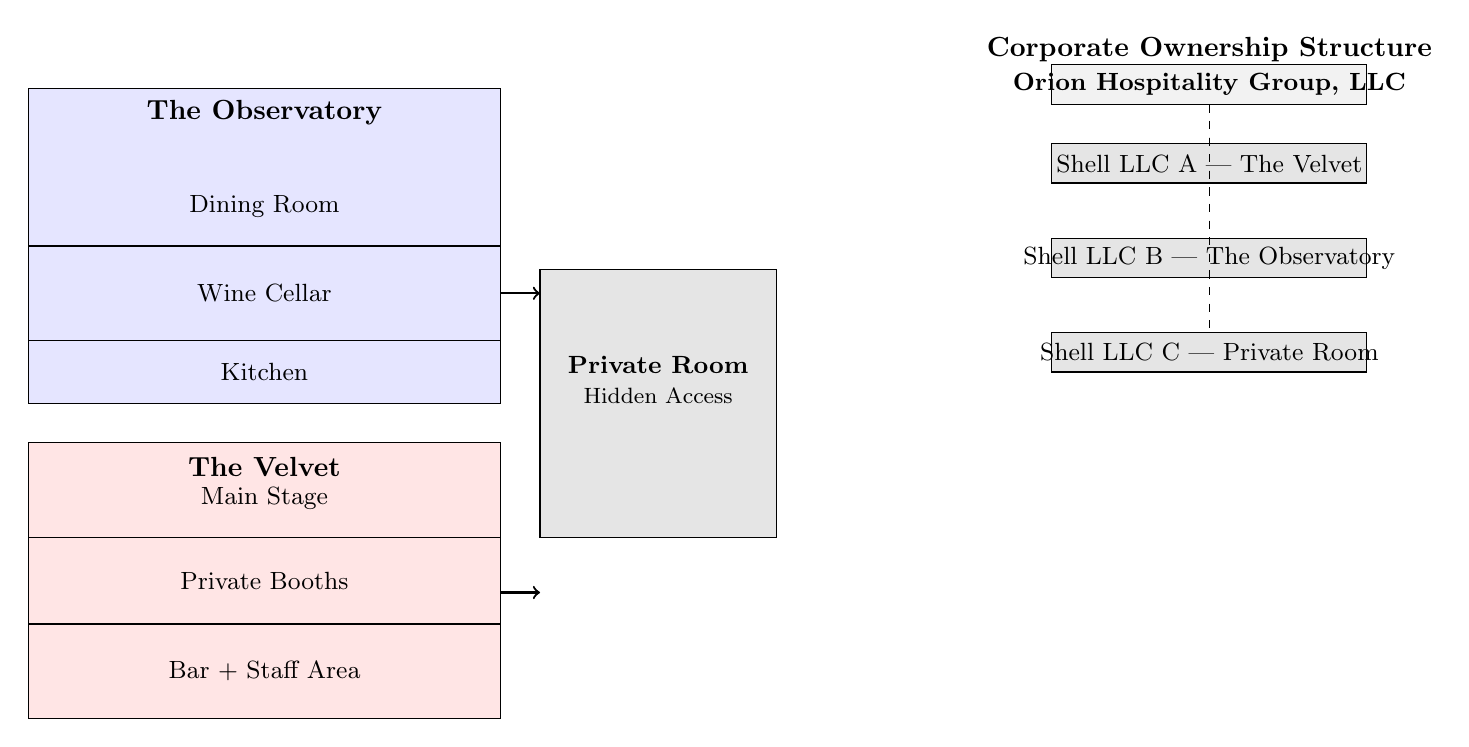
\begin{tikzpicture}[scale=1, font=\small]
  
    % === FLOOR PLAN ===
  
    % The Observatory — 1st Floor Layout
    \draw[fill=blue!10] (0,4) rectangle (6,8); % Restaurant
    \node[font=\bfseries] at (3,7.7) {The Observatory};
    \draw (0,6) -- (6,6); % Divider line
    \node at (3,6.5) {Dining Room};
    \draw (0,4.8) -- (6,4.8);
    \node at (3,5.4) {Wine Cellar};
    \node at (3,4.4) {Kitchen};
  
    % The Velvet — Basement Layout
    \draw[fill=red!10] (0,0) rectangle (6,3.5); % Club
    \node[font=\bfseries] at (3,3.2) {The Velvet};
    \draw (0,2.3) -- (6,2.3);
    \node at (3,2.8) {Main Stage};
    \draw (0,1.2) -- (6,1.2);
    \node at (3,1.75) {Private Booths};
    \node at (3,0.6) {Bar + Staff Area};
  
    % Shared Private Room
    \draw[fill=gray!20] (6.5,2.3) rectangle (9.5,5.7); 
    \node[align=center] at (8,4.3) {\textbf{Private Room}\\\footnotesize Hidden Access};
  
    % Entry arrows to Private Room
    \draw[->, thick] (6,5.4) -- (6.5,5.4); % From wine cellar
    \draw[->, thick] (6,1.6) -- (6.5,1.6); % From booths
  
    % === CORPORATE STRUCTURE ===
    \node[font=\bfseries] at (15,8.5) {Corporate Ownership Structure};
  
    % Parent company
    \draw[fill=black!5] (13,7.8) rectangle (17,8.3);
    \node at (15,8.05) {\textbf{Orion Hospitality Group, LLC}};
  
    % Shells
    \draw[fill=black!10] (13,6.8) rectangle (17,7.3);
    \node at (15,7.05) {Shell LLC A — The Velvet};
  
    \draw[fill=black!10] (13,5.6) rectangle (17,6.1);
    \node at (15,5.85) {Shell LLC B — The Observatory};
  
    \draw[fill=black!10] (13,4.4) rectangle (17,4.9);
    \node at (15,4.65) {Shell LLC C — Private Room};
  
    % Optional: connecting lines (just visual)
    \draw[dashed] (15,7.8) -- (15,7.3);
    \draw[dashed] (15,7.8) -- (15,6.1);
    \draw[dashed] (15,7.8) -- (15,4.9);
  
  \end{tikzpicture}
  \caption{Architectural floor plan of The Observatory (restaurant), The Velvet (club), and a hidden shared private room — all legally separated by distinct shell LLCs but operated under a single parent entity.}
\end{figure}
  
\medskip 

The girls were not staff. But they were not exactly guests, either. The girls were just close 
enough to blur the line, and just far enough to keep anything that happened off the books.

The room itself was equal parts seduction and strategy. On the far side, a 
large circular bed 
slowly revolved under soft amber lights, not fast enough to draw attention, but just enough to suggest movement even when no 
one was on it. Opposite that, a narrow staircase led up to a small balcony lounge with low armchairs and a view that looked 
down over everything: the bed, the tables, and the guests. From up there, the whole scene played like theater.

Beneath the balcony sat a tastefully integrated dancer’s pole that was polished to a mirror finish.
Between the pole and the bed, a row of dark walnut tables offered just enough space for a whiskey flight.
Leather-backed chairs, matte black sugar trays, flickering votives completed the setup, and evoked a high-end coffee shop 
more than a club. It gave cover to whatever the guests chose to call the evening.


After dessert, it wasn’t uncommon for the night to 
migrate there.  Sometimes the wives joined. Sometimes they didn’t.  Sometimes 
they brought their own guests.  On the expense report, it was just a dinner.  It was just a networking event.  
It was just a hospitality line item.  But everyone understood. What happened in the private room wasn’t on the receipt.  
But it was part of the bargain.

If anything compromising happened in that room — a lapse in judgment, a moment of indulgence, a scene that didn’t belong 
in a compliance report — it wouldn’t trace back to the restaurant or the club. Not directly.

The layout made that possible. And so did the paperwork.

The private room acted like a firewall. It was where someone could have a ``business dinner'', and no one would ask questions. 
The circular bed wasn’t just for show, and the mirrored ceiling above it wasn’t an accident. 
Security staff knew where to turn the cameras, and the exit to the Velvet was marked only from the inside. 

\medskip

\begin{TechnicalSidebar}{Significance of a Shell LLC Leasing the Private Room}

  The decision to lease the private room under a shell company wasn’t just legal 
  hygiene. It was structural intent.

  \medskip
  
  First, it created containment. If anything controversial or reputationally toxic happened behind those doors — 
  a lapse in decorum, a breach of ethics, even a crime — liability wouldn’t touch the restaurant or the club. Not 
  directly. On paper, the room belonged to a “private event services firm,” a neutral tenant with no obvious 
  connection to adult entertainment or fine dining. To regulators, auditors, or journalists, the room became a 
  dead end in the org chart.

  \medskip
  
  That insulation granted flexibility. The space could serve multiple roles depending on who was asking. From the 
  restaurant’s side, it might be described as a wine cellar annex or executive dining suite. From the club’s side, 
  it could be pitched as VIP overflow, though never formally listed as part of the venue. And if the conversation 
  was too delicate for either brand to claim, the room could simply be leased out to “external partners” — a 
  euphemism everyone understood.

  \medskip
  
  Then came the deniability. If subpoenas arrived or FOIA requests were filed, staff could answer with complete 
  honesty: that room wasn’t under their control. Access logs, contracts, and invitations all pointed elsewhere. 
  The ambiguity wasn’t a flaw in the structure. It was the feature.

  \medskip
  
  But the real power came in access management. Because the room sat in the jurisdiction of a separate LLC, so 
  did its entry permissions. Key cards, security footage, guest lists were all handled through a different custodial 
  layer. It became a liminal space: technically private, legally detached, and socially malleable. Only insiders 
  understood how fluid the boundary really was.

  \medskip
  
  And finally, there was the financial dimension. A standalone LLC could receive funding through hospitality budgets, 
  bill clients under consulting fees, or depreciate the cost of “client engagement.” Revenues could be rerouted. 
  Expenses could be categorized to fit the desired story. And most importantly, any paper trail would read like a 
  footnote in someone else’s ledger.

  \medskip
  
  This wasn’t just about hiding things. It was about structuring optionality. It was not secrecy for its own sake, 
  but mobility. The kind of mobility that made denial credible, audit trails blurry, and influence hard to trace.
  
\end{TechnicalSidebar}

\medskip

But sex wasn’t the only reason the room existed. That was just the cover.

Its real value came when that same room became the setting for off-calendar meetings. Regulators took calls on encrypted 
phones while pretty girls sat on their laps. Vendors pitched exclusivity clauses without lawyers present. A government 
liaison once reviewed a demo on a tablet between dances.

By law, to avoid conflicts of interest, to preserve impartiality, and to maintain the appearance of independence,
there are situations where \textbf{regulators, auditors, and clients aren’t allowed to share the same room outside
official business}.

But no statute prohibits a regulator from dining at the Observatory, or a client from entering the Velvet. And if they 
happened to meet in the private room? Well, that was just coincidence.

And everyone who entered the room had skin in the game. The cameras weren’t official, but the girls had seen your face. No 
one said it aloud, but the room made sure that what happened there stayed off the record. It made people speak differently. 
It made them speak more candidly. And it made them more open to compromise.

\medskip

\begin{PhilosophicalSidebar}{The Thumbscrew Principle --- Leveraging Mutual Compromise as Insurance}
In high-stakes consulting, reputational risk isn’t always mitigated through compliance—it’s mitigated through 
\textbf{mutual compromise}.  

\medskip

\textbf{Law 33} from \textit{The 48 Laws of Power} explains the underlying psychology:  

\begin{quote}
Discover each man’s thumbscrew.
\end{quote}

In this context, the thumbscrew isn’t leverage from blackmail—it’s the leverage of \textbf{co-participation}. 
You don’t need to threaten exposure if you’ve already pulled them into the same compromising behaviors. Every 
indulgence, every ethical lapse, and every blurred boundary is an insurance policy.  

\begin{quote}
If everyone’s hands are dirty, no one wants to wash them first.
\end{quote}
\end{PhilosophicalSidebar}

\medskip

It wasn’t unusual for a portfolio to be rebalanced while someone’s wife “entertained” multiple men on stage as part of 
the deal itself. For those in the know, her ``performance'' 
\footnote{Her performance carried implications far beyond the surface. It wasn’t just erotic; it was managerial.
Iceberg Slim in his autobiography ``PIMP: My Life'' once described how his mentor taught him how to ``keep a bitch under 
control'': beat her, then give her a cold bath. The comfort
that follows pain, he said, rewires the loyalty. ``She'll be so thankful for the comfort that she'll forget that you were 
the one who hurt her'', he said. In BDSM, they call it ``aftercare''.
In elite circles, they call it ``hospitality''. Either way, it’s the same logic: control wrapped in tenderness.
This wasn’t indulgence; it was choreography. A performance staged to remind the room who offered warmth,
and who could take it away. A performance staged to remind the room who could hurt you, and who could help you.
What’s ``abuse'' when you’re poor becomes ``ritual'' when you’re rich.
What’s trashy in public becomes classy behind French doors.}
was a message disguised as a spectacle to prove her husband's loyalty and compliance.

That was the real purpose: deniability and leverage.

Because in rooms like this, the real power wasn’t in what was said.  It was in what no one dared to say aloud.

\medskip

\begin{figure}[H]
  \centering

  % === First row ===
  \begin{subfigure}[t]{0.45\textwidth}
  \centering
  \begin{tikzpicture}
    \comicpanel{0}{0}
      {Old Pimp}
      {Young Pimp}
      {To keep her loyal, hurt her then be the one to comfort her. She'll call it kindness.}
      {(-0.6,-0.6)}
  \end{tikzpicture}
  \caption*{The lesson: control delivered as a kindness.}
  \end{subfigure}
  \hfill
  \begin{subfigure}[t]{0.45\textwidth}
  \centering
  \begin{tikzpicture}
    \comicpanel{0}{0}
      {Old Pimp}
      {Young Pimp}
      {OK. But what will the cops call it?}
      {(0.6,-0.6)}
  \end{tikzpicture}
  \caption*{The suspicion: wondering what name gets printed on the charge sheet.}
  \end{subfigure}

  \vspace{1em}

  % === Second row ===
  \begin{subfigure}[t]{0.45\textwidth}
  \centering
  \begin{tikzpicture}
    \comicpanel{0}{0}
      {Venture Hostess}
      {Private Guest}
      {His wife fucked the whole room. Then they whispered to her, ``You were radiant.''}
      {(-0.6,-0.6)}
  \end{tikzpicture}
  \caption*{The reenactment: how to package power plays as premium hospitality.}
  \end{subfigure}
  \hfill
  \begin{subfigure}[t]{0.45\textwidth}
  \centering
  \begin{tikzpicture}
    \comicpanel{0}{0}
      {Venture Hostess}
      {Private Guest}
      {Is that aftercare... or just classier pimping?}
      {(0.6,-0.6)}
  \end{tikzpicture}
  \caption*{The question: when power hides behind legal definitions.}
  \end{subfigure}

  \caption*{If you file it under ``team development,'' you can make pimping a corporate expense.}
\end{figure}


\medskip



  



The brilliance wasn’t coercion.  The brilliance was \textbf{slow entanglement}. 
Entanglement so gradual that no single step felt like a compromise.

The Observatory wasn’t a trap door.  It was a funnel lined in velvet.

\begin{quote}
  The real contract wasn’t signed on paper.  The real contract was the months of rooms you shared.
\end{quote}

Hart’s brilliance wasn’t creating leverage over people. It was creating an ecosystem where 
\textbf{everyone had leverage on everyone else}, and thus, no one dared pull the thread.

\medskip

\begin{HistoricalSidebar}{The Broadcom ``Pond'': Henry Nicholas III and the Velvet Trap}

  In the late 1990s and 2000s, tech billionaire \textbf{Henry Nicholas III}, co-founder of Broadcom, wasn’t just making 
  semiconductor chips—he was making headlines for a hidden world beneath his empire.

  \medskip
  
  According to federal prosecutors and court filings, Nicholas built an underground lair beneath his Laguna Niguel warehouse: 
  a secret cave outfitted with a Jacuzzi for six, an \$18{,}000 handcrafted bar, and an Oriental-themed parlor adorned 
  with rugs, statues, and a four-foot Medusa figure. They called it \textbf{“The Ponderosa”} or \textbf{“The Pond.”} 
  Behind a hidden library wall in his mansion, another secret tunnel led to an underground sports bar and recording 
  studio.

  \medskip
  
  But these weren’t just eccentric architectural choices. These were spaces designed for what court filings described as 
  \textbf{marathon drug-fueled orgies}, mixing cocaine, ecstasy, nitrous oxide, prostitutes, and music from Led Zeppelin 
  and Phil Collins in a surreal, days-long bacchanal.

  \medskip
  
  A former employee described the parties: a black box of cocaine sat atop the bar next to a grinder for crushing rocks 
  into powder. A bartender—whom Nicholas had personally sent to bartending school to perfect his favorite cocktail, the 
  \emph{grasshopper}—served guests as they inhaled “whippets” from metal canisters, later replaced by a full nitrous 
  tank when the guests complained the canisters were too cold.

  \medskip
  
  The parties were exclusive, indulgent, and heavily curated. Clients, employees, regulators, and other VIPs were invited 
  to ``network''. A former assistant alleged he was forced to act as a drug courier and to make sure his "friends" were 
  entertained with prostitutes.

  \medskip
  
  When legal troubles surfaced, no formal charges of blackmail or hostage-taking emerged, but the \textbf{dynamic of 
  mutual compromise was clear}:  

  \begin{quote}
    Everyone inside the cave had a stake in the silence.  Everyone left with something they couldn’t easily admit.  
  \end{quote}
  
  Nicholas didn’t need overt threats. The space itself was the leverage. Participation was the insurance policy.  

  \medskip
  
  And when a regulator, client, or associate later hesitated to follow his lead, the implication wasn’t spoken, but it 
  was understood:  \textit{“We were in the cave together.”}

  \medskip
  
  His case ended with dropped charges, plea deals, and no prison time. But the broader lesson lingers: Nicholas built 
  more than a secret room—he built a velvet trap, where the real power wasn’t what he held over others, but what they 
  already held over themselves.

  \medskip

  And the final irony?
  
  \medskip

  After years of drugs, prostitutes, and corruption swirling beneath the radar, what finally brought authorities to his 
  doorstep wasn’t the cave’s activities—it was a noise complaint from neighbors, triggered when Nicholas tried to expand 
  his secret sex dungeon without a building permit by hiring undocumented Mexican laborers to excavate it in secret.

  \begin{quote}
  ``The Pond'' survived the long arm of the law, but it couldn’t survive the long arm of the home owner's association.
  \end{quote}

\end{HistoricalSidebar}

\medskip

It wasn’t about written agreements, enforceable terms, or formal obligations. It was about weaving participants into a 
\textbf{mutual dependency of silence}, a tacit agreement built not on paper but on complicity.

Every invitation to an off-book dinner, every casual introduction to a “friend of the firm,” and every night where boundaries 
blurred wasn’t just a favor. It was a stitch in the fabric of a collective secret. A secret that tied everyone 
together in a web where exposure couldn’t be isolated. To expose anyone else was to expose yourself.

The genius of this ecosystem wasn’t overt coercion. It was self-reinforcing compliance. Once inside, no one wanted to 
be the first to speak. And no one wanted to be the first to walk away. Because leaving clean required admitting you were 
never clean.

This is the architecture of \textbf{distributed leverage}:  No single actor holds absolute power over the others because 
everyone holds just enough dirt to keep the group stable. It mirrors the principle of \emph{mutually assured destruction}, 
but at the level of reputation and informal loyalty rather than military force.

\medskip

\begin{PsychologicalSidebar}{Distributed Leverage and the Psychology of Pluralistic Ignorance}

  In 1931, social psychologist \textbf{Floyd Allport} first coined the term \emph{pluralistic ignorance} to describe a 
  curious phenomenon: a group of individuals might all privately disagree with a norm or practice, yet publicly uphold 
  it because they mistakenly believe everyone else supports it.
  \medskip

  Later, researchers like \textbf{Daniel Katz} and \textbf{Floyd Allport} expanded the concept through experimental 
  studies, showing how this false consensus effect sustains unethical or undesirable group behavior—not through overt 
  coercion, but through collective misperception.

  \medskip

  In Hart’s ecosystem, pluralistic ignorance wasn’t just an incidental byproduct—it was engineered.

  \medskip

  Each private dinner, each informal introduction, each blurry night of implicit favors created a shared assumption: 
  \textbf{“Everyone else is comfortable with this. Everyone else is playing along.”}

  \medskip

  But beneath the surface, many participants might have felt uneasy. The genius of the system was that no one could 
  tell. Silence became the default, not because everyone agreed, but because no one wanted to be the first to admit 
  discomfort.

  \medskip

  And with every silent nod, the ecosystem hardened. Each individual believed departure would mean revealing not just 
  their own doubts—but their own complicity.

  \medskip

  Psychologists studying pluralistic ignorance found that the longer such a norm persists unchallenged, the stronger 
  it feels --- even if privately, no one endorses it.

  \begin{quote}
    The brilliance of distributed leverage isn’t enforcing consensus.  It’s making each individual believe consensus 
    already exists.
  \end{quote}

\end{PsychologicalSidebar}

\medskip

Hart didn’t merely sell access. He didn’t merely sell deals. He sold membership in a system that rewrote the very 
rules of accountability.

\begin{quote}
  Because a cartel doesn’t need to control the market if it controls the consequences of leaving.
\end{quote}

And the more entangled you became, the harder it was to chart a path back to independence. Why? Because every bridge out 
had already been soaked in the gasoline of shared participation.

Hart’s real product wasn’t strategy, capital, or connections.  
Hart’s real product was the invisible web.  
\textbf{It was a structure where participation became the only viable strategy.}

\medskip

\begin{HistoricalSidebar}{Enron, Strip Club Lu, and the Audit that Never Happened}

  In the early 2000s, as the collapse of \textbf{Enron} shook global markets, a secondary casualty followed: 
  \textbf{Arthur Andersen}, once one of the “Big Five” accounting firms, disintegrated under the weight of 
  complicity.  

  \medskip
  
  The natural question lingered: \textit{How did the auditors miss it?}  

  \medskip
  
  Then the stories of \textbf{“Strip Club Lu”} surfaced.  
  
  \medskip
  
  Lu, an Enron executive, had become notorious across Houston’s nightlife scene. His nickname wasn’t ironic. 
  It was literal. Lu was known for throwing down so much cash at strip clubs that you couldn’t see the floor 
  under the dollar bills. And the best part?  \textbf{It was all expensed.}  

  \medskip
  
  Officially filed under “research,” Lu’s excursions weren’t solo adventures. He brought \textbf{clients}, 
  \textbf{partners}, and even \textbf{auditors} along for the ride. What began as networking spiraled into 
  bacchanals of absurd excess.  
  
  \medskip
  
  When the \textbf{SEC investigation} later combed through emails, they uncovered something even darker: 
  multiple warnings from Enron’s internal compliance officer, \textbf{Sherron Watkins}, and from other 
  executives like \textbf{David Skilling} (nicknamed “Skelleg” in internal memos), begging Lu to stop 
  using Enron’s offices for after-hours parties.  

  \medskip
  
  The emails weren’t vague: they referenced \textbf{orgies in the office with strippers}, documented 
  concerns about security footage, and outright pleas to stop turning corporate headquarters into a 
  late-night adult playground.  
  
  \medskip
  
  And yet, within the industry, everyone knew.  

  \medskip
  
  Stories about Enron’s “hospitality” weren’t whispered—they were \textbf{bragged about}. Competitors joked 
  about partnering with Enron just to enjoy the legendary parties. Visiting investment bankers told stories 
  of the corporate Amex being swiped for champagne fountains. And behind it all, Arthur Andersen’s auditors 
  kept signing off on the books.  
  
  \medskip
  
  The brilliance (if it can be called that) wasn’t a cover-up. It was \textbf{mutual indulgence}.  
  
  \begin{quote}
  When everyone’s at the party, no one wants to turn on the lights.
  \end{quote}
  
  Enron’s collapse wasn’t just a financial failure. It was a case study in what happens when complicity becomes 
  cultural currency, and reputational risk is managed through \textbf{mutual dirt}.  
  
  \begin{quote}
  The real audit wasn’t the one filed in the reports.  
  The real audit was the chain of silent approvals signed with every swipe of the card.
  \end{quote}
  
  In the end, Arthur Andersen didn’t fail because they didn’t know.  Arthur Andersen failed because they did.
  
\end{HistoricalSidebar}

\medskip

That’s why Hart chose this room for the real conversation.  
Not because it was private.  
But because it was preloaded with consent.

Leather walls. No windows. A table just small enough to keep everyone close.  
And a bottle of Japanese whiskey in the center.

David sat across from him, with Paolo — the regulator liaison — at his side.  
And flanking them, always within reach, were the girls from the gentleman's club.

\medskip

\begin{PhilosophicalSidebar}{Regulatory Capture — When Oversight Learns to Speak Client}

  In theory, regulators exist to safeguard the public interest — ensuring that safety, transparency, and fairness 
  override private ambition.  
  But in practice, something quieter often unfolds: oversight doesn’t disappear. It \textit{assimilates}.  

  \medskip
  
  This is the essence of \textbf{regulatory capture}.

  \medskip
  
  Not bribery. Not threats.  
  Just proximity. Familiarity. The soft erosion of boundaries through shared incentives and shared vocabulary.
  
  \medskip
  
  \textbf{Paolo} wasn’t just a liaison — he was a translator.  
  The bridge between regulatory opacity and startup ambiguity.  
  He’d spent years mastering the dialect of both sides: how to phrase a model’s interpretability risk as a “technical 
  opacity window,” how to reframe edge-case failures as “innovation latitude.”
  
  \medskip
  
  Hart didn’t need Paolo to sign off.  
  He needed him to nod at the right moments.  
  To offer a “soft read” on which clauses might trigger scrutiny.  
  To hint at how far the edges of compliance could stretch without snapping.
  
  \medskip
  
  Officially, Paolo wasn’t allowed to shape deployment timelines.  
  Unofficially, he could signal just how much regulatory slack they had — and how quietly a deployment might slide 
  through under an innovation exemption.

  \medskip
  
  That’s why he was in the room.

  \medskip
  
  Not to approve.  
  Not to object.  
  But to observe — and later, to forget just enough of what he saw.
  
  \medskip
  
  This is how capture works:  
  Not through malice, but through \textbf{mutual alignment}.  
  The regulator begins to see the world not as it is — but as the client wants it to be.  
  What starts as interpretation becomes advocacy.  
  What starts as oversight becomes choreography.
  
  \begin{quote}
  The danger isn’t that the watchdog falls asleep.  
  It’s that he learns the pitch deck.
  \end{quote}
  
\end{PhilosophicalSidebar}

\medskip


One girl draped her arm casually over Hart’s shoulder. She brushed his lapel with a faux-absentminded touch.  
Another leaned in to refill David’s glass with her nails tapping lightly on the stem as she steadied it.  
The perfume shifted every time someone moved. He smelled musk, citrus, and smoke.  

It wasn’t a formal pitch. But it wasn’t casual either.

At the time, David didn’t question the setting.  
He chalked it up to Hart’s signature flair. The curated decadence. The blurred line between deal and indulgence.
It is what everyone came to expect.  

The room was just private enough to lower one’s guard, and just dim enough to dull consequence.  
And the girls were warm, playful, and always half-involved. 
They gave the whole scene the texture of safety.  
The girls made it feel like no one would remember what was said, so long as no one wrote it down.

But later, he would understand.

\textit{This wasn’t just where the deal happened.}  

\textit{This was where something crossed a line.}

He didn’t sign a document that night.  
But he said something he shouldn’t have.  

He agreed to something he wasn’t ready for.  
Because he let the room decide for him.

And by the time he realized why Hart had chosen this room —  
with its erotic silence and curated distractions —  
it was too late to walk it back.

The lighting in the back room of the club was low, not out of modesty but design.  Everything was upholstered 
in softness: velvet cushions, silk dresses, and practiced smiles.

Hart leaned back with one arm resting along the top of the table and the other wrapped around a glass of 
scotch that seemed never to empty. “We’ve already routed exposure through the model at Arcadia,” he said, smiling. 
“It’s holding up beautifully under stress.”

One of the girls giggled, not at the words, but at the warmth in Hart’s tone. She whispered something into his ear. 
But he didn’t break eye contact with David.

David said nothing. Not because he agreed. But because correcting Hart would have meant introducing friction. And the 
room had been designed to punish friction. Everything here was buffered: light, sound, and dissent.

A girl walked past and trailed her hand along the back of Paolo’s chair. Paolo didn’t flinch, either because he didn’t 
notice or because he knew not to.

Paolo turned to David. “Impressive,” he said. “So it’s in live deployment?”

David hesitated. Not because the answer was complicated, but because another woman had leaned gently against the edge 
of the table beside him. She let her fingers trail along his thigh, featherlight. It was more suggestion than touch. 
More strategy than affection.

“We’re...” David adjusted in his seat. “Finalizing interpretability for regulated clients. Some edge-case volatility 
around correlation breaks. But nothing that would preclude a limited pilot.”

He hated how the words sounded coming out of his mouth. It was technically true, but also incomplete. But the truth 
wasn’t the currency here.

Because by the time David realized it, they hadn’t just partnered with Centauri.

They’d been \textbf{acquired in all but paperwork}.

Another girl returned with drinks and slipped into the space beside Hart. She perched like a bird trained to rest on 
expensive shoulders. Her smile was more curated than warm.

“We’ve got two desks looking to replace their quant overlays by Q3,” Paolo said casually. “If the stability’s there, 
we could slip it in under their innovation mandate.”

David looked up. He should’ve said no. He should’ve said “Q4 at the earliest.” He should’ve said “We haven’t passed 
adversarial stress.”

But instead, he nodded. Not because the system was ready, but because the social machinery was already in motion. 
He was no longer being asked to evaluate a deployment schedule.

He was being asked if he belonged.

\begin{quote}
Paolo expects this. Paolo was brought into the loop with you. Paolo smiled at you across the table while the 
deal was forming.
\end{quote}

To push back now would not be a technical objection. It would be a social betrayal.

“That’s doable,” David said.

Hart raised his glass. The girl beside him clinked hers against his without being asked.

“To velocity,” Hart said smoothly, “and to teams that don’t wait for permission.”

They all clinked glasses.  
Paolo smiled.  
The woman beside David leaned close enough to break the threshold where lapse in judgement 
turns into impulse. So when she leaned in, he mistook her presence for peace.

And with a nod, a sip, a sentence he couldn’t take back,  
and a moment of silence that smelled like perfume...
David had just approved the deployment.

Then David swallowed his scotch like a confession.
Not to release it, but to trap it somewhere deeper.

But the burn wasn’t enough.

That's why when she kissed him, he kissed her back.

But he did not kiss her out of want.

He kissed her to forget --- for the moment --- that this burden was his alone to carry.

It was not desire. And it was not connection. 

It was anesthesia with a pulse.

\medskip

\begin{PhilosophicalSidebar}{Professional Ethics, Conflict of Interest, and the Structure of Trust}

  At the heart of professional ethics lies not morality, but preservation. Professional ethics is not about individuals
  morality, but about the profession itself.

  \medskip
  
  Engineers, doctors, and lawyers are held to a higher standard not because they are inherently more virtuous, but because 
  the public must believe they are. Without trust in the profession, the system that relies on them collapses.

  \medskip
  
  
  This is why a doctor is delicensed for intentionally harming a patient, even if they believe it’s ``for their own good.''
  This is why a lawyer is disbarred for lying to a judge, even if it secures the client’s victory. The damage is not just to 
  the case, but to the credibility of the legal system itself. The punishment isn't about wrongdoing: it’s about maintaining 
  the fiction that professionals serve truth, and not their employer.

  \medskip
  
  
  Across industries, entire regulatory architectures are built to separate power from practice. Medical administrators may 
  oversee budgets, but they are legally barred from dictating medical decisions. Project managers handle scope and timelines, but 
  not engineering decisions. Corporate lawyers can direct business strategy, but cannot ignore legal obligations without 
  putting the company — and the entire profession — at risk.

  \medskip
  
  
  In situations of conflict, a professional must invoke a higher loyalty: \textit{professional ethics}. A doctor must say, 
  ``I cannot do that, even if the CEO asks.'' A lawyer must say, ``I serve the law first.'' An engineer must say, ``That shortcut 
  would compromise safety.'' Their oath binds them not to the client, but to the discipline itself.

  \medskip
  
  In essence: \textbf{Ethics begins where control ends.}

  \medskip
  
  To protect a profession, you must give its members the authority to say no, and the obligation to mean it.
  
\end{PhilosophicalSidebar}


\subsection{Editor Questions for ``The Room Without a Name''}

To get meaningful and diverse feedback, I designed these questions to go beyond surface-level edits. 
Please reflect not only on technical clarity or style, but on emotional tone, character depth, pacing, 
moral ambiguity, and thematic structure. Don’t feel pressure to answer every question. Focus on the 
ones that resonate most with your experience as a reader. The goal isn’t to clean up the prose — it’s 
to understand how the story lands, where it connects, and where it quietly unsettles.

\subsubsection{Narrative \& Structure}

\begin{itemize}
  \item Did the scene build tension in a way that felt organic? Was the payoff earned?
  \item Was the pacing too fast, too slow, or just right?
  \item Were the flashbacks and sidebars effective in deepening your understanding, or did they disrupt the flow?
\end{itemize}

\subsubsection{Emotional Impact}

\begin{itemize}
  \item Did you feel anything for David — sympathy, frustration, complicity?
  \item Were you emotionally affected by the moment David approved the deployment? Why or why not?
  \item Did the final paragraph land for you as a turning point?
\end{itemize}

\subsubsection{Psychological Depth}

\begin{itemize}
  \item Did the internal conflict David experienced feel real and human?
  \item Was the concept of “velvet funnel” clear in its psychological implication?
  \item Did you believe the way David rationalized his choices in the moment?
\end{itemize}

\subsubsection{Sidebar Effectiveness}

\begin{itemize}
  \item Did the historical and philosophical sidebars feel integrated or intrusive?
  \item Was there a sidebar that clarified or recontextualized the main narrative for you?
  \item Would you prefer fewer sidebars, more, or placement elsewhere?
\end{itemize}

\subsubsection{Thematic Reflection}

\begin{itemize}
  \item What do you think this scene is ultimately about?
  \item Did the ideas of complicity, distributed leverage, or ethical erosion resonate with you?
  \item What real-world institutions or dynamics did this section remind you of?
\end{itemize}

\subsubsection{Style \& Language}

\begin{itemize}
  \item Were there any lines or images that stood out (positively or negatively)?
  \item Did the writing feel immersive or overly stylized?
  \item Did the tone match the gravity of what was happening?
\end{itemize}

\subsubsection{Optional: Deeper Testing}

\begin{itemize}
  \item If you had to explain this chapter to someone else in one sentence, what would you say?
  \item If this were the only chapter you read, what genre or world would you think the book is part of?
  \item What would you cut or condense if you needed to trim 10–20\%?
\end{itemize}








\subsection{The Black Swan}

Eventually, the event came.

\textbf{It was a margin call.}

It was a full-blown liquidity spiral. 

It was the financial version of a crowded theater where someone yells ``fire,'' and the 
exits are narrower than anyone remembered.

But here’s the twist:
The fire alarm wasn’t faulty. 
It worked.
In fact, it was the very thing the system claimed to be monitoring — the signal that was supposed to give everyone early 
warning — that triggered the panic.

  \medskip

\begin{PhilosophicalSidebar}{When the Fire Alarm Starts the Fire}

  In a rational world, warning systems reduce harm.  
  They give you time to respond, to plan, to adapt.

  \medskip
  
  But in complex systems — like financial markets, logistics networks, or algorithmically governed institutions — 
  that assumption breaks down.  
  The \textbf{alarm} doesn’t just inform behavior.  
  It \textit{coordinates} it.
  
  \medskip
  
  And when everyone gets the same signal at the same time, they don’t calmly adjust.  
  They panic in sync.
  
  \medskip
  
  This is the paradox of modern risk architecture:  
  The very tools designed to prevent systemic collapse can accelerate it. And not necessarily because they’re 
  wrong, but because they’re \textbf{too right}, too fast, and too widely trusted.

  \medskip
  
  
  It’s what George Soros called \textit{reflexivity}:  
  When perceptions change reality, and reality reinforces perception.  
  A widening credit spread doesn’t just reflect stress. It \textit{becomes} the stress.  
  A model warning doesn’t just highlight fragility. It \textit{triggers} it.
  
  \medskip
  
  From a philosophical standpoint, this is a problem of \textbf{second-order knowledge}.  
  It’s not just what you know. It’s what you know others know, and what they will do with that knowledge.  
  The signal doesn’t just forecast the future. It becomes part of the causality.
  
\end{PhilosophicalSidebar}

  \medskip


Imagine a smart building with a state-of-the-art earthquake detection system. Except one day, it picks up a tremor, 
automatically locks the elevators, shuts down the exits, blasts a siren, then causes a stampede. 
The stampede did not happen because the earthquake 
was severe, but because the system reacted so fast, and so confidently, that no one questioned it.

That’s what happened here.

The risk models saw rising interest rates or a sudden shift in commodity flows — something real, but manageable — and lit up 
the dashboard. But their very act of alerting, in a world primed for panic, created the very instability they were supposed 
to guard against.

Because once everyone receives the same “early warning” signal at the same time, the market doesn’t hedge — it herds.

Liquidity vanishes. Safe assets get dumped to cover losses. Correlations converge to one. And what started as a modest 
risk event becomes a self-fulfilling spiral.

So no, this wasn’t a stress test.
It was the system stress-testing itself, and failing in live fire.


\medskip

\begin{TechnicalSidebar}{Margin Calls --- From Prudence to Predation}

  %\textbf{Origin: Safety Mechanism.}  
  Margin calls began as a conservative financial tool in the early 20th century, formalized after the 1929 crash. 
  The idea was simple: if your position loses too much value, you must deposit more collateral or sell. It was 
  designed to prevent systemic failure by stopping runaway losses before they spread.

  \medskip
  
  %\textbf{1934: Regulation T.}  
  The U.S. Securities Exchange Act of 1934 established limits on how much credit could be extended to purchase 
  stocks, giving birth to official margin requirements. The purpose was stability — to avoid a recurrence of the 
  speculative bubbles that had fueled the Great Depression.

  \medskip
  
  %\textbf{The Shift: From Protection to Pressure.}  
  In modern markets, margin calls still serve their protective role. However, they also act as triggers. When markets 
  are calm, leverage multiplies returns. But when volatility spikes, margin calls can create forced selling, which 
  pushes prices lower, which triggers more margin calls. The result? A feedback loop of liquidation.

  \medskip
  
  %\textbf{Abuse by Design.}  
  Today, high-frequency firms and leveraged hedge funds often model margin call chains not as risks to avoid, but 
  as moves to exploit. A firm with early insight into margin pressure can front-run the collapse, short the 
  liquidity vacuum, and profit from the forced unwinding of others.
  
  \medskip
  
  %\textbf{And the AI didn’t even blink.}  
  What was once a circuit breaker is now a lever. In the hands of algorithms, it’s not a warning... it’s a weapon.
  
\end{TechnicalSidebar}

\subsection{Editor Questions for ``The Black Swan''}

This scene is where the theoretical becomes real. The abstract fears of earlier chapters materialize into a coordinated crisis. 
It’s also a philosophical turn — a meditation on systems that collapse under the weight of their own design. The questions 
below aim to test how this section lands — as narrative, as insight, and as structural escalation.

\subsubsection{Narrative \& Escalation}

\begin{itemize}
  \item Did the crisis scene feel earned based on what came before?
  \item Did the explanation of how the system collapsed feel believable — or too convenient?
  \item Was the metaphor (fire alarm triggering panic) effective? Did it clarify or distract?
\end{itemize}

\subsubsection{Emotional Stakes}

\begin{itemize}
  \item Did this section make you feel anything — dread, recognition, cynicism, awe?
  \item Was there a moment where the emotional weight really landed for you?
  \item Did the tone match the gravity of a systemic breakdown, or did it feel too detached?
\end{itemize}

\subsubsection{Philosophical Sidebar}

\begin{itemize}
  \item Did the “Fire Alarm Starts the Fire” sidebar deepen your understanding of the reflexivity concept?
  \item Was the idea of second-order knowledge and market perception clear, or did it need more grounding?
  \item Did this sidebar integrate well with the narrative moment, or would you prefer it embedded differently?
\end{itemize}

\subsubsection{Technical Sidebar}

\begin{itemize}
  \item Did the margin call history and logic provide helpful context for what happened?
  \item Was the transition from safety mechanism to predatory strategy convincing?
  \item Were there any terms or concepts that felt too dense or needed clarification?
\end{itemize}

\subsubsection{Thematic Insight}

\begin{itemize}
  \item What do you think this chapter is ultimately arguing about financial systems or predictive models?
  \item Did the self-fulfilling nature of the collapse feel plausible? Chilling? Overstated?
  \item Were there any real-world parallels that immediately came to mind while reading this?
\end{itemize}

\subsubsection{Style \& Craft}

\begin{itemize}
  \item Were the images or metaphors (e.g., smart building stampede, fire alarm) memorable?
  \item Was the balance of exposition and storytelling effective?
  \item Did anything in the prose feel repetitive, heavy-handed, or overly intellectualized?
\end{itemize}

\subsubsection{Optional: Stress Testing the Section}

\begin{itemize}
  \item If you had to cut 15\% of this section, what would go first?
  \item If you had to simplify this for a less technical reader, what would you change?
  \item If this scene came earlier in the book, how would it change your interpretation of what follows?
\end{itemize}


\subsection{The Reflexive Cascade}

Aurora didn’t miss the signals.  
It flagged early tremors: volatility clustering, thinning liquidity, subtle correlation drift.  
The model did what it was trained to do — synthesize complexity, identify stress, and issue a call to rebalance.

Arcadia acted.  
It moved out of high-beta exposures.  
Rotated across synthetic baskets.  
Reallocated through ETF proxies and volatility-hedged credit structures.

\medskip

\begin{TechnicalSidebar}{ETFs --- From Access to Abstraction}

  The first modern ETF — the SPDR S\&P 500 Trust (SPY) — launched in 1993, offering everyday investors access to a 
  diversified basket of stocks with a single trade. It was built on a simple idea: give people passive exposure to the 
  market without paying active managers to lose their money.

  \medskip
  
  ETFs quickly gained traction. They were transparent, liquid, and cheap. Institutions loved them for hedging. Retail 
  investors loved them for simplicity. By the early 2000s, ETFs had exploded across asset classes: bonds, commodities, 
  emerging markets, even volatility itself.

  \medskip
  
  But not all ETFs are baskets of real stuff. Many are \textbf{synthetic} — engineered with derivatives to track complex 
  exposures. Leveraged and inverse ETFs, for example, use swaps and futures to magnify returns (and losses), sometimes 
  resetting daily, often with massive slippage over time.

  \medskip
  
  Just as \textbf{Liar’s Poker} chronicled how Goldman Sacks sliced, repackaged, and resold mortgage bonds to clueless investors, 
  modern ETFs have spawned a similar game — this time with volatility swaps, CDS indices, and leveraged factor models. 
  The packaging is cleaner, but the risks are just as hidden.

  \medskip
  
  Firms like \textbf{Arcadia Capital} used ETFs to express exotic macro views with a single click, and sometimes unaware that 
  the liquidity of the ETF didn’t match the liquidity of the underlying assets. When stress hit, bid-ask spreads widened, 
  NAVs diverged, and redemption pressure triggered forced unwindings.

  \medskip
  
  \textbf{And the AI?}  
  It flagged volatility.  
  It flagged dispersion.  
  It never asked whether the instrument itself was the risk.
  
\end{TechnicalSidebar}

\medskip

No alarms.  
No headlines.  
Just quiet, precise adjustments — the kind that usually stay invisible.

Except they didn’t.

Arcadia’s trades — routed through liquid ETFs and structured exposures — left a footprint.  
The flows registered.  
Market-makers noticed imbalances.  
Bid-ask spreads widened.  
NAVs diverged from price.

\begin{TechnicalSidebar}{Market Makers and the Mirage of Liquidity}

  The term \textbf{market-maker} sounds neutral — even helpful.  
  In theory, market-makers provide liquidity by continuously quoting both buy and sell prices (bid and ask), allowing trades to happen smoothly, even in volatile markets.
  
  \medskip
  
  But in practice, “market-maker” often masks something more opportunistic.

  \medskip
  
  Many modern market-makers — especially in fragmented or lightly regulated environments — do more than just quote prices.  
  They observe client flows, detect intent, and trade ahead of size. This is known (politely) as \textbf{anticipatory liquidity provision}, and (less politely) as \textbf{front-running}.
  
  \medskip
  
  When a large institution like Arcadia starts moving structured exposure through ETFs,  
  market-makers don’t need a whistleblower to see it. They see it in the order book.
  
  \medskip
  
  \textbf{What happens next?}
  
  \begin{itemize}
    \item They widen spreads before the full trade executes.
    \item They adjust internal models to account for expected flow continuation.
    \item In some cases, they take the other side temporarily — only to unwind with better pricing moments later.
  \end{itemize}
  
  This creates an illusion of liquidity — one that vanishes the moment too many players lean on it.
  
  \medskip
  
  In Arcadia’s case, the footprint left by ETF unwinds became visible — not just to analysts,  
  but to trading algorithms programmed to infer institutional distress.  
  This visibility accelerated slippage, triggered further margin recalibration,  
  and turned what should have been a quiet rotation into a broadcasted panic.
  
  \medskip
  
  \textbf{The irony?}  
  The very infrastructure meant to ensure smooth execution became the amplifier of fragility.

  \medskip
  
  Because sometimes, “market-maker” isn’t a role.  
  It’s a pretext — for watching, reacting, and profiting at the speed of inference.
  
\end{TechnicalSidebar}


What the platform hadn’t accounted for was this:

The instruments were abstract — synthetic baskets, volatility overlays, cross-asset ETFs —  
but the effects were real.  
And real doesn’t mean smooth.  
It means sharp, recursive, reflexive.

\medskip

Arcadia’s unwind began methodically.  
No panic. No forced liquidation.  
Just a quiet, Aurora-guided rotation out of energy-heavy and credit-tilted exposures.

The platform had promised discretion.  
It had promised dynamic execution, risk balancing, and portfolio-level coherence —  
all without sending signals into the market.

But that’s not what happened.

\medskip

Aurora’s trades routed through ETFs.  
And ETFs route through market-makers — Citadel, Jane Street, Flow Traders —  
firms whose job isn’t just to provide liquidity, but to \textit{recognize patterns} and 
\textit{price risk before it appears}.

The flows lit up dashboards.

Internal algos flagged Arcadia’s pattern as stress-induced.  
Spreads widened preemptively.  
Liquidity shifted from “available” to “contingent.”  
And in a market wired for inference, that was enough.

\medskip

The model hadn’t broken.  
But the promise had.

Aurora had assured Arcadia that its execution logic would adapt to market conditions —  
that the platform would stagger trades, conceal intention, and avoid footprint.

Instead, Arcadia became the footprint.  
Aurora’s optimizations had become legible — not just to Arcadia, but to the street.

\medskip

Soon, the reaction loop took hold:

\begin{itemize}
  \item Liquidity providers pulled quotes on structurally similar ETFs.
  \item Market-makers pre-hedged flow continuation, front-running Arcadia’s own trades.
  \item Options desks repriced implied vol — breaking hedge assumptions baked into the model.
\end{itemize}

Aurora kept monitoring.  
Arcadia kept trusting.  
But trust has a half-life.  
And Aurora never flagged the shift — not because it failed to see, but because it never thought to look there.

The irony?

The system had promised to manage exposure.  
But it had no visibility into the second-order effects of its own footprint.

\textit{The trades were clean. The execution wasn’t.}

By week’s end, the model still showed internal consistency.  
Risk scores hadn’t spiked. Correlation matrices held.

But Arcadia’s pnl told a different story.

The thing Aurora hadn’t modeled — and never disclosed —  
was that in a market governed by machine-readable flow,  
predictable behavior \textit{is} exposure.

So no, the model didn’t malfunction.  
But it violated its core promise: to act intelligently and invisibly.

And what looked like execution... \textit{was a broadcast.}

Not a fire.  
\textit{A hall of mirrors.}
And Arcadia never saw the reflection coming.


\subsection{Editor Questions for ``The Reflexive Cascade''}

This section dives into feedback loops — not just in markets, but in visibility, trust, and machine-readable behavior. 
It’s quieter than a crash, but arguably more dangerous because it masks fragility in the language of precision. 
The questions below are designed to help you test how well this subtle complexity lands.

\subsubsection{Narrative \& Pacing}

\begin{itemize}
  \item Did the pacing of this unwind feel convincing — too fast, too slow, or just right?
  \item Were the transitions between narrative and technical sidebars fluid or jarring?
  \item Did the scene maintain narrative tension despite the absence of overt drama?
\end{itemize}

\subsubsection{Systemic Logic}

\begin{itemize}
  \item Did you clearly understand how Arcadia’s own behavior created the conditions for its unraveling?
  \item Was the link between ETF trades and visibility to market-makers well-explained?
  \item Did the concept of reflexivity (in this case, machine-readable flow) come through effectively?
\end{itemize}

\subsubsection{Technical Sidebar Clarity}

\begin{itemize}
  \item Did the ETF sidebar clarify or confuse the idea of synthetic exposures and liquidity mismatch?
  \item Was the distinction between ``instrument risk'' and ``execution risk'' made clear?
  \item Was there anything you felt should be expanded or cut for clarity?
\end{itemize}

\subsubsection{Market Microstructure Insight}

\begin{itemize}
  \item Did the explanation of market-makers’ behavior feel realistic or too cynical?
  \item Did you grasp how spread widening, pre-hedging, and front-running were triggered by Arcadia’s own footprint?
  \item Were you left with a clearer understanding of how execution platforms can become exposures?
\end{itemize}

\subsubsection{Theme \& Message}

\begin{itemize}
  \item What do you think this chapter is ultimately critiquing — the tech, the trust, or the illusion of control?
  \item Did the phrase ``the trades were clean. the execution wasn’t'' resonate as a summary?
  \item Did the “hall of mirrors” metaphor feel earned or overstated?
\end{itemize}

\subsubsection{Style \& Craft}

\begin{itemize}
  \item Was there a line or image that really stayed with you?
  \item Did the interplay of technical precision and emotional distance heighten or flatten the reading experience?
  \item Did anything feel overwritten, or like it could be simplified without losing nuance?
\end{itemize}

\subsubsection{Optional: Deeper Testing}

\begin{itemize}
  \item If this scene were adapted for screen or stage, what would be the emotional or visual climax?
  \item Would this section benefit from a contrasting voice or perspective (e.g., from a junior trader or compliance)?
  \item If this section had ended in a total blow-up instead of a silent erosion, would the message have landed stronger or weaker?
\end{itemize}





\subsection{The Portfolio That Looked Safe — Until It Didn’t}

On paper, Arcadia’s positioning was elegant.  
Tactically asymmetric.  
Algorithmically justified.  
Optimized — not by instinct, but by Aurora.

The platform had surfaced the opportunity:  
Go \textbf{long energy} — via commodity-linked ETFs —  
and hedge with a \textbf{short position on investment-grade credit}, executed synthetically through CDS indices.

Classic convexity.  
If oil rose, energy rallied.  
If spreads widened, the CDS paid out.  
One leg offsets the other.  
Clean. Modeled. Risk-controlled.

But clean models assume clean separations.  
Markets, especially stressed markets, do not.

The trigger wasn’t extraordinary.  
A sharper-than-expected 120 basis point hike in short-term rates — sharp, but not unprecedented.  
In past cycles, it would have caused some rotation, a few red screens. Not this.

But this time, the instruments were different — and so was the execution.

\begin{itemize}
  \item The long leg was implemented through leveraged ETFs — fast in, faster out.
  \item The short leg was expressed via CDS — derivatives tied to corporate credit, not actual bond exposure.
  \item Both positions were cross-margined — their liquidity modeled, but never truly tested.
\end{itemize}

When oil dropped, the energy leg collapsed.  
Because it was leveraged, losses were nonlinear — exponential.  
Margin calls arrived within the hour.

Aurora responded just as it was designed to:  
Rebalance. Reallocate. Raise liquidity.

So Arcadia sold what was most liquid — or at least, what Aurora’s liquidity engine said was:  
\textbf{Investment-grade ETFs.}

But the sale pressure didn’t go unnoticed.  
Market-makers picked it up instantly.  
The trades looked coordinated, the flows had signature.  
Not panic, but intent.

Spreads widened.  
NAVs decoupled from price.  
And the credit hedge — the part that was supposed to protect the portfolio — began bleeding too.

Because Aurora’s models had assumed independence.  
But the street had connected the dots.

The CDS indices, now mispriced relative to bond volatility, moved the wrong way.  
Arcadia faced variation margin on its hedge; even as it was still absorbing losses on its core.

\textit{The offset became exposure. The hedge became a blade.}

\textbf{The result?}

\begin{itemize}
  \item The energy bet turned toxic.  
  \item The short hedge became a second source of drawdown.  
  \item The “safe” assets became the flashpoint for systemic inference.
\end{itemize}

And Aurora?

It never flagged the contagion.  
Because its execution logic assumed liquidity, and its trust model assumed invisibility.  
But market-makers had seen the flow.  
They had adjusted.  
They had widened spreads and front-loaded risk before the platform could respond.

The model hadn’t just underestimated the correlation risk.  
It had created it — through transparency, through predictability, through faith.

So when the cascade unfolded, it wasn’t because the strategy was wrong.  
It was because too many desks were following the same logic,  
with tools designed to be safe — but not designed to be seen.

\textit{It wasn’t a risk model failure.}  
It was a reflexive misfire — one that began the moment Arcadia trusted Aurora to move without being noticed.


\medskip

\begin{figure}[H]
  \centering
  \resizebox{\textwidth}{!}{%
  \begin{tikzpicture}[node distance=1.5cm and 3cm, every node/.style={font=\small}]
  
  % Nodes
  \node[draw, align=center, fill=gray!10] (trigger) {Macro Trigger:\\\textbf{120bps rate hike}\\\textbf{+ Oil flash crash}};
  \node[draw, below=of trigger, fill=gray!10, align=center] (plunge) {\textbf{Oil futures collapse}\\$\downarrow$14\% in 30 min};
  \node[draw, below=of plunge, fill=gray!10, align=center] (portfolio) {Arcadia Portfolio:\\\textbf{Long oil and}\\\textbf{Short IG via CDS}};
  \node[draw, below=of portfolio, fill=gray!10, align=center] (margincall) {\textbf{Trigger margin calls}\\on futures positions};
  \node[draw, below left=of margincall, fill=gray!10, align=center] (liqbonds) {\textbf{Sells}\\\textbf{investment-grade bonds}\\to raise cash};
  \node[draw, below right=of margincall, fill=gray!10, align=center] (cdsspread) {\textbf{IG bond spreads widen}\\$\Rightarrow$ CDS short loses value};
  
  \node[draw, below=of margincall, fill=gray!10, align=center] (variation) {\textbf{Variation margin calls}\\from credit counterparties};
  
  % Arrows
  \draw[->, thick] (trigger) -- (plunge);
  \draw[->, thick] (plunge) -- (portfolio);
  \draw[->, thick] (portfolio) -- (margincall);
  \draw[->, thick] (margincall) -- (liqbonds);
  \draw[->, thick] (margincall) -- (cdsspread);
  \draw[->, thick] (cdsspread) -- (variation);
  
  % Feedback loop
  \draw[->, thick, dashed, bend left=30] (variation.north) to node[right, align=center] {\scriptsize More margin calls\\\scriptsize $\Rightarrow$ More selling} (margincall.south);
  
  \end{tikzpicture}
  }
  \caption{Cascade triggered by rate shock and oil crash: how feedback loops undid Arcadia.}
\end{figure}

\subsection{Editor Questions for ``The Portfolio That Looked Safe — Until It Didn’t''}

This section explores how precision engineering — in financial models, hedge construction, and execution platforms — can create fragility when assumptions fail. These questions aim to surface whether that fragility was felt, understood, and earned.

\subsubsection{Narrative \& Structure}

\begin{itemize}
  \item Did the sequence of events feel clear and causally connected?
  \item Was the pacing of the unraveling effective — too fast, too slow, or just right?
  \item Did the transition to the TikZ figure help you visualize the collapse or feel redundant?
\end{itemize}

\subsubsection{Financial Logic \& Clarity}

\begin{itemize}
  \item Was the long/short strategy (energy vs. credit) understandable even if you’re not a finance expert?
  \item Did the explanation of CDS, leveraged ETFs, and cross-margining feel coherent?
  \item Did you understand why the hedge failed — and how the model's logic contributed?
\end{itemize}

\subsubsection{Systemic Risk \& Reflexivity}

\begin{itemize}
  \item Did the feedback loop — from margin calls to forced sales to hedge breakdown — feel plausible?
  \item Did you grasp how visibility and predictability became vulnerabilities?
  \item Was the phrase ``the hedge became a blade'' effective in conveying the turn?
\end{itemize}

\subsubsection{Theme \& Message}

\begin{itemize}
  \item What do you think this scene is ultimately critiquing — leverage, opacity, automation, or institutional trust?
  \item Did the notion of ``reflexive misfire'' make sense as a failure mode?
  \item Do you feel this is a story about risk, or a story about belief in systems?
\end{itemize}

\subsubsection{Writing \& Craft}

\begin{itemize}
  \item Was there a line or metaphor that stood out — positively or negatively?
  \item Did the tone strike the right balance between technical and narrative?
  \item Were there moments of repetition or density that could be streamlined?
\end{itemize}

\subsubsection{Optional: Deeper Testing}

\begin{itemize}
  \item If this section were adapted into a documentary, what visual elements would be most critical to capture?
  \item Would the piece benefit from more human perspective (e.g., a PM reacting in real time)?
  \item How would this scene land differently if you didn’t understand the financial mechanics — would it still be compelling?
\end{itemize}





\subsection{The Volatility of Peace}


\textbf{What broke it was what no one expected: peace.}

For weeks, global markets had been pricing in conflict — like a casino full of gamblers who'd all heard the same rumor 
about a rigged roulette wheel. The rumor? That a critical energy corridor was about to become a geopolitical parking 
lot: a drawn-out standoff, sanctions flying, ports slowed to a crawl, and oil tankers idling in tense waters. 

The bet was simple: if supply gets choked then prices go up.

If oil futures surged then crude flirted with triple digits.

\medskip

\begin{TechnicalSidebar}{What’s a Future, Anyway?}

  A \textbf{futures contract} is a financial agreement to buy or sell something — oil, wheat, interest rates, even 
  weather — at a predetermined price on a specific future date.

  \medskip
  
  You don’t have to want the thing itself.  
  You’re trading the \textit{price of belief} — what the market thinks something will be worth in the near future.
  
  \medskip
  
  Originally, futures were for hedging:  
  A farmer locks in a price before harvest. An airline locks in fuel costs before summer.  
  They’re trying to protect against uncertainty.

  \medskip
  
  But today?  
  Most futures are traded by people who don’t want the commodity at all.  
  They want the volatility. The leverage. The signal.
  
  \medskip
  
  When traders “go long” on oil futures, they’re betting that prices will rise.  
  When they “short” futures, they’re betting they’ll fall.  
  But beneath every bet is a narrative: a rumor, a headline, a geopolitical twitch.

  \medskip
  
  And when everyone hears the same rumor — like a war or supply choke — the entire market starts tilting the same way.  
  That tilt becomes the price.
  
  \medskip
  
  So when crude surged and futures “priced in conflict,” they weren’t just reflecting the world.  
  They were \textit{constructing} it — one bet at a time.
  
\end{TechnicalSidebar}

\medskip


Investment desks positioned themselves accordingly. 
Energy portfolios were stacked with long positions — the financial equivalent of stockpiling canned food before a hurricane. 
Hedge funds placed leveraged bets. 
Sovereign wealth funds adjusted allocations. 
Even cautious family offices, the financial turtles of the investing world, crept into the action, 
betting on the storm lasting.

But here’s the catch:
\textbf{All these trades were modeled on the assumption of gridlock.}
That nothing would move. That diplomacy would fail. That energy would become the world’s next great bottleneck.

\medskip

\begin{figure}[H]
  \centering
  \begin{tikzpicture}[scale=1.1]
  
    % Nodes for regions
    \node[draw, fill=blue!10, minimum width=2cm, minimum height=1cm, rounded corners] at (-5, 0) (Americas) {Americas};
    \node[draw, fill=green!10, minimum width=2cm, minimum height=1cm, rounded corners] at (0, 2) (Europe) {Europe};
    \node[draw, fill=yellow!10, minimum width=2cm, minimum height=1cm, rounded corners] at (4, 0) (Asia) {Asia};
    \node[draw, fill=orange!10, minimum width=2cm, minimum height=1cm, rounded corners] at (0, -2) (Mideast) {Mideast};
  
    % -- Conflict Scenario (gray dashed reroutes) --
    \draw[->, thick, dashed, gray] (Americas.east) .. controls (-2,0.5) .. (Europe.west) node[midway, above, font=\scriptsize, gray] {rerouted};
    \draw[->, thick, dashed, gray] (Europe.east) .. controls (2,1.5) .. (Asia.west);
    \draw[->, thick, dashed, gray] (Asia.south west) .. controls (2.5,-1.5) .. (Mideast.east);
  
    % -- Peace Scenario (bold reactivated routes) --
    \draw[->, thick, blue] (Americas.east) .. controls (-1,1.5) .. (Asia.west) node[midway, above, font=\scriptsize, blue!70!black] {reactivated};
    \draw[->, thick, blue] (Mideast.north) -- (Europe.south) node[midway, right, font=\scriptsize, blue!70!black] {normal flow};
  
    % Blocked zone icon (conflict assumption)
    \draw[thick, red] (0.5,-0.4) circle (0.4cm);
    \node[red, font=\scriptsize] at (0.5,-1.1) {Chokepoint};
  
    % Peace unlocked symbol
    \node[font=\Large, blue!80!black] at (0.5,-0.4) {\checkmark};
  
    % Caption
    \node[align=center, font=\small, text width=10cm, below=2.5cm of Mideast.south] {
      \textbf{Market Assumptions:} Trade routes blocked due to conflict (gray, dashed)\\
      \textbf{What Happened:} Routes reopened suddenly (blue, solid) as diplomacy unexpectedly succeeded.
    };
  
  \end{tikzpicture}
  \caption{Simplified trade flow map: models priced in conflict and rerouting, but peace reactivated critical corridors and shocked market expectations.}
\end{figure}

\medskip

In trading terms, this was a textbook ``consensus narrative'': a shared story that underwrites the price of everything 
from oil futures to airline stocks. It’s like everyone agreeing the bridge ahead is broken and adjusting their GPS 
routes accordingly. If that bridge suddenly reopens? Chaos. Price reversion. And margin calls for anyone who bet too 
heavily on detours.

In short: the markets weren't just betting on oil.
They were betting on stalemate.
And when stalemates break, so do assumptions.

\medskip

\begin{PhilosophicalSidebar}{The Consensus Narrative}

  Markets don’t just price assets.  
  They price stories.

  \medskip
  
  A \textbf{consensus narrative} is the shared fiction everyone agrees to believe — not because it's true, but because 
  it’s \textit{useful}.  Like money. Like borders. Like market confidence itself.
  
  \medskip

  In theory, prices are objective: functions of supply, demand, and discounted cash flows.  
  In practice, they’re often anchored to collective expectations — war drags on, interest rates stay flat, demand rebounds, 
  volatility remains containable.

  \medskip
  
  When those expectations are stable, so are markets.  
  But consensus isn’t knowledge. It’s choreography.  
  Everyone adjusts their models not to reality, but to what they think others believe reality will be.
  
  \medskip
  
  This is where philosophy meets finance.  
  David Hume warned that causality itself is inferred — not seen.  
  Thomas Kuhn showed how science advances through “paradigm shifts,” not incremental truth.  
  And George Soros built a hedge fund empire on reflexivity — the idea that markets move not toward reality, but toward the 
  beliefs they manufacture and reinforce.
  
  \medskip
  
  So when traders say “the market priced in a stalemate,” they don’t mean it’s true.  
  They mean it’s operationally assumed.

  \medskip
  
  The danger?  
  Consensus narratives are stable — until they’re not.  
  When the story breaks, the model doesn’t just shift.  
  It collapses.  

  \medskip
  
  And that collapse doesn’t just create volatility.  
  It creates \textbf{epistemic whiplash} — the sudden, violent shock of realizing the map wasn’t the territory.
  
\end{PhilosophicalSidebar}

\medskip


Then came the de-escalation.

A late-night diplomatic breakthrough. A surprise joint statement. Military assets stood down. Trade routes reopened. 
Within minutes, satellite imagery confirmed what the markets had feared to believe: the tankers were moving again.

\textbf{And with that, oil collapsed.} Not gradually. Not rationally.

\textbf{Oil futures dropped 14\% in thirty minutes.}


It was the kind of move risk models usually assign a probability so low, they round it down to zero.  It’s like getting 
struck by lightning while winning the lottery during an eclipse. Technically conceivable, but not worth planning for.

And yet, it happened.

The geopolitical script flipped overnight. The expected standoff didn’t materialize. A backchannel opened. A surprise 
deal was inked. Or a missile landed just a few pixels off from the scenario desk's baseline. Whatever the trigger, it 
defied the assumptions every model had quietly baked in.

And just like that, the market re-priced violently.

Imagine a packed theater where the audience has been told the fire alarm is just part of the show, and then someone 
yells “actual fire.” The rush for the exits isn’t graceful. 

Because in markets, when a "zero-probability" event comes true, it's not just a plot twist:
\textbf{it's a regime change.}

\medskip

\begin{figure}[H]
  \centering
  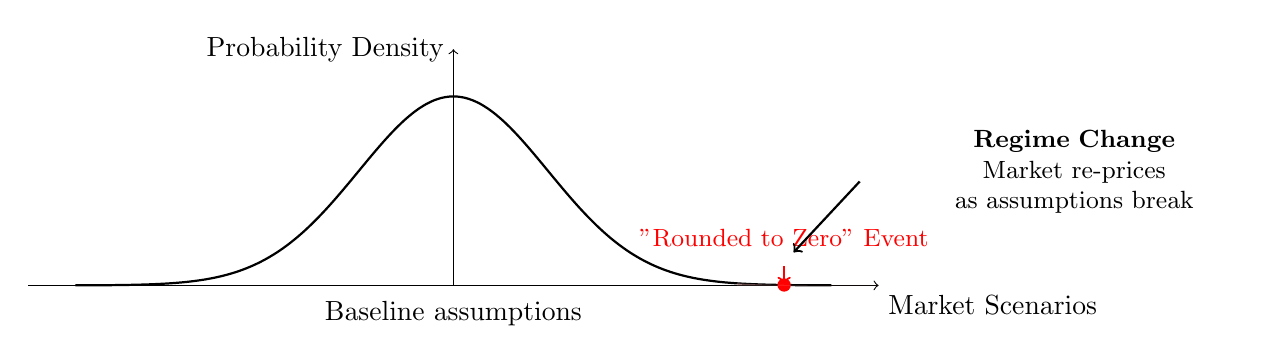
\begin{tikzpicture}[scale=1.2]
    % Bell curve
    \draw[->] (-4.5,0) -- (4.5,0) node[below right] {Market Scenarios};
    \draw[->] (0,0) -- (0,2.5) node[left] {Probability Density};
  
    % Normal distribution curve
    \draw[thick, smooth, domain=-4:4, samples=100] 
      plot(\x, {2*exp(-0.5*\x*\x)}) node[right] {};
  
    % Label for center
    \node at (0,-0.3) {Baseline assumptions};
  
    % Extreme tail event
    \fill[red] (3.5,{2*exp(-0.5*3.5*3.5)}) circle (2pt);
    \draw[->, thick, red] (3.5,{2*exp(-0.5*3.5*3.5) + 0.2}) -- (3.5,{2*exp(-0.5*3.5*3.5) + 0.01});
    \node[red, above] at (3.5,{2*exp(-0.5*3.5*3.5) + 0.3}) {\small "Rounded to Zero" Event};
  
    % Shaded tail
    \fill[red!30, opacity=0.4] (3.0,0) -- plot[domain=3:4.5] (\x, {2*exp(-0.5*\x*\x)}) -- (4.5,0) -- cycle;
  
    % Annotation of regime change
    \node[align=center, text width=4cm, right, font=\small] at (4.8,1.2)
      {\textbf{Regime Change}\\Market re-prices\\as assumptions break};
  
    \draw[->, thick] (4.3,1.1) -- (3.6,0.35);
  
  \end{tikzpicture}
  \caption{Visualizing a low-probability, high-impact event: when “rounded-to-zero” scenarios become reality, the market experiences a nonlinear regime shift.}
\end{figure}

\medskip

But that wasn’t the only surprise: Credit spreads blew out, but not where the models were looking.

In financial terms, a “credit spread” is like an insurance premium. 
It’s how much extra return an investor demands to lend money to a risky borrower instead of a safe one. 
When spreads “blow out,” it means people suddenly see more risk and demand more compensation to take it on.
It is like an earthquake making everyone scramble to check their home insurance policy.

\medskip

\begin{TechnicalSidebar}{Credit Spreads and the Anatomy of a Blowout}
  In traditional finance, a \textbf{credit spread} measures the difference in yield between a corporate bond and a risk-free government bond of comparable maturity. It reflects the market’s perception of default risk. A higher spread signals higher perceived risk; a lower spread suggests confidence in repayment.
  
  \medskip
  
  \textbf{The Baseline:}  

  \medskip

  If the U.S. 10-year Treasury is yielding 2.0\% and a corporate bond yields 6.0\%, the credit spread is:
  \[
  6.0\% - 2.0\% = 4.0\%
  \]

  \medskip
  
  This 4.0\% “risk premium” compensates investors for the possibility of default.
  
  \medskip
  
  \textbf{What’s a Blowout?}  

  \medskip

  A \textbf{credit spread blowout} occurs when spreads widen rapidly across a category of borrowers; especially high-yield or speculative-grade issuers. It often precedes or coincides with a liquidity crisis, as lenders demand dramatically higher yields or refuse to roll debt entirely.
  
  \medskip
  
  \textbf{Historical Blowouts:}

  \medskip

  \begin{itemize}
    \item \textbf{2008 Financial Crisis:} Spreads on junk bonds exceeded 2,000 basis points (20\%), reflecting panic over cascading defaults.
    \item \textbf{COVID-19 March 2020:} Even investment-grade spreads widened dramatically until the Fed intervened with corporate bond purchases.
  \end{itemize}

  \medskip
  
  \textbf{Why it Matters:}  

  \medskip

  A spread blowout doesn’t just reflect risk. It creates it. It signals that markets are no longer willing to fund at previous terms. For leveraged firms, that can trigger a debt rollover crisis, margin calls, or forced liquidation — especially when \textbf{credit was being used to simulate liquidity}.

\end{TechnicalSidebar}

\medskip

But here’s the twist: The quake didn’t hit where the seismographs were pointed.

Traders had positioned themselves around the obvious fault lines: energy companies, defense contractors, and countries caught 
in the geopolitical blast radius. The models were calibrated to stress those areas. Risk was priced-in there.

But the actual rupture came somewhere else — maybe in a shipping company that relied on a now-sanctioned route, or a regional 
bank exposed to commodities financing. It was like boarding up your windows for a hurricane, only to have the roof collapse 
from termites you didn’t even know were there.

That’s the danger of overfitting to a single scenario: the risk doesn’t vanish; it just moves offscreen.

When the unexpected sector starts flashing red, credit spreads widen there, liquidity dries up, and everyone who thought 
they were safe suddenly isn’t. The models weren’t wrong because they were bad.  They were wrong because the world refused 
to stay inside the prediction box.

\medskip

\begin{figure}[H]
  \centering
  \begin{tikzpicture}
    \matrix[matrix of nodes,
            nodes={minimum height=1cm, minimum width=1.8cm, text width=1.8cm, align=center},
            column sep=0.1cm, row sep=0.1cm,
            cells={nodes={draw, font=\small}}] (m) {
      |[fill=red!70]| Energy & |[fill=orange!30]| Shipping & |[fill=green!10]| Regional Banks & |[fill=yellow!20]| Real Estate & |[fill=green!10]| Tech \\
      |[fill=orange!20]| Energy & |[fill=red!70]| Shipping & |[fill=red!60]| Regional Banks & |[fill=yellow!30]| Real Estate & |[fill=green!10]| Tech \\
    };
  
    % Labels
    \node[font=\bfseries] at ($(m-1-1.north west)!0.5!(m-1-5.north east)+(0,1)$) {Expected Credit Spread Stress};
    \node[font=\bfseries] at ($(m-2-1.south west)!0.5!(m-2-5.south east)+(0,-1)$) {Actual Credit Spread Stress};
  
    % Color legend
    \begin{scope}[shift={(7.2,-0.5)}]
      \node[align=left, font=\small] at (0,1.2) {Stress Level};
      \draw[fill=green!10] (0,0.8) rectangle ++(0.4,0.4);
      \node[anchor=west, font=\tiny] at (0.5,1.0) {Low};
  
      \draw[fill=yellow!30] (0,0.3) rectangle ++(0.4,0.4);
      \node[anchor=west, font=\tiny] at (0.5,0.5) {Moderate};
  
      \draw[fill=red!70] (0,-0.2) rectangle ++(0.4,0.4);
      \node[anchor=west, font=\tiny] at (0.5,0.0) {High};
    \end{scope}
  \end{tikzpicture}
  \caption{Heatmap of Expected vs. Actual Credit Spread Movement. Models focused on obvious sectors (e.g., Energy), but market stress materialized in overlooked areas like Shipping and Regional Banks.}
\end{figure}

\medskip

Most risk engines — the predictive models used by banks, funds, and regulators — had been trained on the usual suspects.
They were like airport security trained to spot people with ticking suitcases and shady passports. The algorithms knew how to 
flag high-yield bonds from companies drowning in debt, or cyclical sectors like manufacturing and construction that wobble 
with every interest rate shift. These models were fluent in the language of fragility — companies with weak balance sheets, 
volatile revenues, or exposure to economic booms and busts.

But this time, the pressure hit from the blind side.

Instead of the usual weak links snapping, the stress landed on investment-grade borrowers — supposedly sturdy, reputable firms 
— who happened to rely on commodity-linked income or had large footprints in markets that were suddenly back in play after 
years of sanctions. These weren’t the people with ticking suitcases. These were the ones wearing business class tags and 
tailored suits. And when turbulence hit them, no one saw it coming.

Why? Because the models had only seen one version of history.

\medskip

\begin{figure}[H]
  \centering
  
  % === First row: Conflict Shock ===
  \begin{subfigure}[t]{0.45\textwidth}
  \centering
  \begin{tikzpicture}
    \comicpanel{0}{0}
      {Risk Model}
      {Macro Analyst}
      {Rising tension. Sanctions expected. Volatility will spike in energy and defense.}
      {(-0.6,-0.6)}
  \end{tikzpicture}
  \caption*{Conflict shock: the volatility is forecast, localized, and priced in.}
  \end{subfigure}
  \hfill
  \begin{subfigure}[t]{0.45\textwidth}
  \centering
  \begin{tikzpicture}
    \comicpanel{0}{0}
      {Macro Analyst}
      {Risk Model}
      {Contagion risk remains in the usual suspects: cyclicals, high-yield, frontier markets.}
      {(0.6,-0.6)}
  \end{tikzpicture}
  \caption*{The usual drill: stress ripples through known fault lines.}
  \end{subfigure}
  
  \vspace{1em}
  
  % === Second row: Peace Shock ===
  \begin{subfigure}[t]{0.45\textwidth}
  \centering
  \begin{tikzpicture}
    \comicpanel{0}{0}
      {Risk Model}
      {Macro Analyst}
      {Ceasefire? Trade lanes reopening? This wasn't in the training data.}
      {(-0.6,-0.6)}
  \end{tikzpicture}
  \caption*{Peace shock: the models aren’t built to process resolution.}
  \end{subfigure}
  \hfill
  \begin{subfigure}[t]{0.45\textwidth}
  \centering
  \begin{tikzpicture}
    \comicpanel{0}{0}
      {Macro Analyst}
      {Risk Model}
      {Credit spreads just blew out in investment-grade shipping. Why now?}
      {(0.6,-0.6)}
  \end{tikzpicture}
  \caption*{The misfire: volatility hits where “peace” broke the assumptions.}
  \end{subfigure}
  
  \caption*{Markets don’t just panic when things get worse. Sometimes they panic when things get better.}
\end{figure}

\medskip

They had been trained on past crises where breakdowns came slow — grinding recessions, dragged-out wars, and slow-motion defaults. 
Like a chess player who's only practiced defensive endgames, they weren’t ready for what came next: a sharp reversal, and a 
geopolitical twist that defused tension rather than inflamed it. In short: they had prepared for escalation, not resolution.

The underlying math — the assumptions about how risk spreads from one part of the system to another — was based on the idea 
that bad news spreads quickly and good news doesn’t spread at all. That volatility comes from conflict, and contagion from 
collapse. But this time, the trigger wasn’t an explosion. It was a handshake. And that broke the logic the models were built on.

In market terms, it was like every fire drill having trained people to flee from smoke, and then discovering that some doors 
slam shut when the alarm is turned off.
Peace, it turns out, can cause a stampede too.

Because when the world rewires faster than the models can adapt, even safety can become a liability.
And those who bet on disorder... suddenly find themselves out of position when the chaos doesn’t arrive.

Because peace doesn’t usually cause flash crashes.  \textit{Until it does.}

\medskip

\begin{figure}[H]
  \centering
  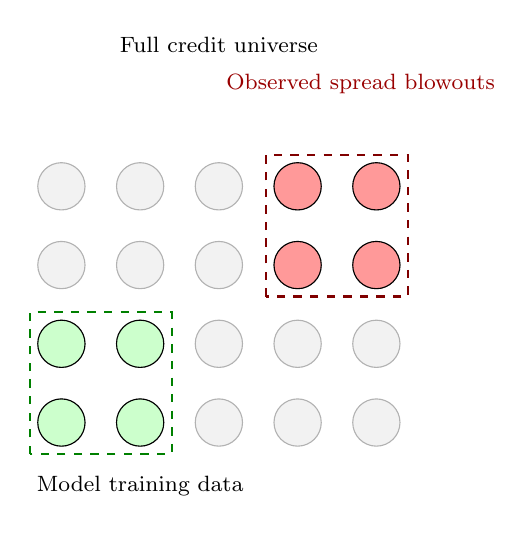
\begin{tikzpicture}[
      model/.style={circle, draw=black, fill=green!20, minimum size=0.6cm},
      blowout/.style={circle, draw=black, fill=red!40, minimum size=0.6cm},
      neutral/.style={circle, draw=black!30, fill=gray!10, minimum size=0.6cm},
      every node/.style={font=\scriptsize}
  ]
  
  % Credit universe grid (5x4)
  \foreach \x in {0,1,2,3,4} {
      \foreach \y in {0,1,2,3} {
          \node[neutral] (n\x\y) at (\x, \y) {};
      }
  }
  
  % Model training region (bottom-left 2x2)
  \foreach \x in {0,1} {
      \foreach \y in {0,1} {
          \node[model] at (\x, \y) {};
      }
  }
  
  % Blowout region (top-right 2x2)
  \foreach \x in {3,4} {
      \foreach \y in {2,3} {
          \node[blowout] at (\x, \y) {};
      }
  }
  
  % Labels
  \node[align=left, font=\footnotesize] at (1, -0.8) {Model training data};
  \node[align=left, font=\footnotesize, text=red!60!black] at (3.8, 4.3) {Observed spread blowouts};
  \node[align=left, font=\footnotesize] at (2, 4.8) {Full credit universe};
  
  \draw[dashed, thick, green!50!black] (-0.4, -0.4) rectangle (1.4, 1.4);
  \draw[dashed, thick, red!50!black] (2.6, 1.6) rectangle (4.4, 3.4);
  
  \end{tikzpicture}
  \caption{Spread Blowout Occurred Outside Model Coverage: The model was trained on credit names in calm regimes (green), but the shock hit an unmodeled set of issuers (red).}
\end{figure}

\medskip

The AI never flagged this because it had learned from historical data that IG bonds and oil weren’t highly correlated.  
It assumed the CDS short would \textit{offset} the oil exposure.

Instead, both positions bled simultaneously.

The selling fed on itself.  
As prices dropped, margin requirements recalibrated mid-day.  
Auroras’s model, trained on low-volatility environments, continued recommending small rebalances instead of issuing 
a halt.

\begin{itemize}
  \item By 2:30 p.m., Arcadia had received four sequential margin calls.  
  \item By 3:15 p.m., they had begun liquidating equity positions to cover margin on the credit book.  
  \item By 4:00 p.m., they were locked out of their own OMS, triaging via phone.
\end{itemize}

Aurora issued a severity alert, but only after 89\% of daily liquidity had already dried up.

\medskip

\begin{figure}[H]
  \centering
  \resizebox{\textwidth}{!}{%
  \begin{tikzpicture}[
    node distance=1.2cm and 2.2cm,
    every node/.style={font=\small},
    box/.style={draw, rounded corners, minimum width=3.8cm, minimum height=1.2cm, align=center, fill=gray!10},
    arrow/.style={->, thick}
  ]
  
  % Top layer (assumptions)
  \node[box] (data) {Narrow Training Data\\(Low-volatility, stable regime)};
  \node[box, right=of data] (assumption) {Learned Historical\\Decorrelation};
  \node[box, right=of assumption] (blindspot) {No Calibration for\\Joint Stress Events};
  
  % Middle layer (stress response)
  \node[box, below=2cm of blindspot] (shock) {Oil Collapse \& CDS Spread Blowout\\Ignored as Uncorrelated};
  \node[box, left=of shock] (margin) {Margin Calls Trigger Forced Selling};
  \node[box, left=of margin] (amplify) {Selling Widens Spreads\\Triggers More Margin Calls};
  
  % Bottom layer (outcomes)
  \node[box, below=2cm of margin] (late) {AI Issues Alert\\After 89\% Liquidity Is Gone};
  \node[box, right=of late, fill=red!20] (result) {\textbf{Catastrophic Losses}\\Portfolio -47\%};
  
  % Arrows (top layer)
  \draw[arrow] (data) -- (assumption);
  \draw[arrow] (assumption) -- (blindspot);
  
  % Arrows (top → middle)
  \draw[arrow] (blindspot.south) -- (shock.north);
  \draw[arrow] (shock) -- (margin);
  \draw[arrow] (margin) -- (amplify);
  
  % Arrows (middle → bottom)
  \draw[arrow] (amplify.south) -- (late.north);
  \draw[arrow] (late) -- (result);
  
  \end{tikzpicture}
  }
  \caption{Three-stage breakdown: flawed assumptions, failure under stress, and financial collapse.}
\end{figure}
  
\medskip


\subsection{Editor Questions for ``The Volatility of Peace''}

This section explores how financial markets can misfire not only from unexpected conflict, but also from unexpected resolution. These questions are designed to probe the effectiveness of the narrative, the coherence of the financial mechanics, and the resonance of the larger thematic message.

\subsubsection{Narrative \& Structure}
\begin{itemize}
  \item Did the section feel coherent as a single arc, or more like a sequence of vignettes?
  \item Was the use of sidebars and visual elements additive, or did they fragment the flow?
  \item Did the ending ("Peace doesn’t usually cause flash crashes. Until it does.") feel earned or too stylized?
\end{itemize}

\subsubsection{Emotional \& Cognitive Impact}
\begin{itemize}
  \item Did the inversion of expectations (peace causing a crisis) land for you?
  \item Were there moments that made you pause and reflect — either about markets or about belief systems?
  \item Did you experience any confusion about causality, or did the cascade of events feel clear?
\end{itemize}

\subsubsection{Financial Logic \& Comprehension}
\begin{itemize}
  \item Was the role of futures, CDS, and credit spreads explained accessibly?
  \item Did the diagrams (e.g., bell curve, spread grid) help solidify your understanding?
  \item Was the idea of a "regime change" in markets made intuitive?
\end{itemize}

\subsubsection{Thematic Resonance}
\begin{itemize}
  \item What do you think this section is ultimately about: risk, reflexivity, overfitting, or something else?
  \item Did the concept of "epistemic whiplash" help frame the deeper message?
  \item Did it provoke any broader philosophical questions for you about how we model or expect the world?
\end{itemize}

\subsubsection{Style \& Craft}
\begin{itemize}
  \item Were there lines or metaphors that stood out (positively or negatively)?
  \item Was the use of humor (e.g., "getting struck by lightning during an eclipse") effective or distracting?
  \item Did the prose balance precision with accessibility?
\end{itemize}

\subsubsection{Optional: Structural Testing}
\begin{itemize}
  \item If this section were cut in half, what would you keep?
  \item Would a character perspective (e.g., a trader, PM, or analyst reacting in real time) improve the tension?
  \item If you hadn’t read the title, when would you have realized this wasn’t a war story, but a peace one?
\end{itemize}




\subsection{The Collapse}

The next morning, Arcadia’s portfolio \textbf{NAV was down 47\%}.

\medskip

\begin{HistoricalSidebar}{The Cult of NAV}

  \textbf{NAV}, or \textit{Net Asset Value}, was originally a mundane accounting tool. It is a snapshot 
  of what a portfolio was worth if you sold everything, paid off the debts, and called it a day.

  \medskip
  
  But in the late 20th century, NAV became something more: a totem of institutional legitimacy. Hedge funds, 
  mutual funds, venture portfolios — all started tethering their credibility to this fluctuating number, 
  updated obsessively, audited reluctantly, and weaponized politically.

  \medskip
  
  When Arcadia’s NAV dropped 47\% overnight, it wasn’t just a financial event. It was a reputational implosion: 
  the kind that could empty boardrooms, evaporate term sheets, and trigger frantic calls from LPs who didn’t 
  remember what they signed up for.

  \medskip
  
  NAV pretends to be objective. But it’s part oracle, part theater: a number everyone believes in, until they 
  don’t. And when they stop believing then it becomes the reason they run.
  
\end{HistoricalSidebar}

\medskip

Nearly half the fund’s value was incinerated before breakfast.

There was no breaking news alert. No Bloomberg headline. Just silence.
The kind of silence that creeps across a trading floor like smoke.

Slack channels slowed.
Risk dashboards froze.
The models—usually precise, sometimes smug—began returning garbage:
Negative prices, vanishing liquidity, and volatilities that made no statistical sense.

Some bonds simply stopped trading.
Others had no consensus price—just wide, surreal spreads and no takers.
An IG credit marked at 88 the night before now showed a bid at 74—if you could find one.
One trader muttered, “This looks like ‘08 pricing.”
No one corrected him. No one laughed.

\textbf{Two counterparties had already seized collateral.}

Not a phone call. Not even an email.
Just auto-executed clauses buried deep in long-forgotten ISDA annexes.

\medskip

\begin{TechnicalSidebar}{What’s in an ISDA Annex?}

  At first glance, an ISDA agreement looks like a partnership.

  \medskip
  
  But it isn’t.

  \medskip
  
  It’s a legal machine — and the annexes are where the machine learns how to bite.
  
  \medskip
  
  The \textbf{ISDA Master Agreement} is the boilerplate. It governs the relationship and defines the rules. But the real leverage lives in the attachments:

  \medskip
  
  \begin{itemize}
    \item \textbf{Schedule A}  
    Custom terms. This is where counterparties bury modifications, exceptions, and definitions that override the defaults. Want to enable collateral sweeps during market stress? You don’t change the master — you bury it in Schedule A, Paragraph 13.2(c).
  
    \item \textbf{Credit Support Annex (CSA)}  
    This governs margin. It spells out which assets count as collateral, how often they’re revalued, and how quickly they must be posted or returned. It also defines what happens when the market stops cooperating.
  
    \item \textbf{Definitions Booklets}  
    A running catalog of what technical terms mean (e.g., “Close-Out Amount,” “Eligible Collateral,” “Valuation Agent”). Updated over time. Seemingly trivial — until you realize that a clause like “reasonable discretion” can move \$100 million in five minutes.
  
    \item \textbf{Confirmations}  
    Trade-by-trade terms. These are the receipts — the specific transactions that inherit all the machinery above them.
  \end{itemize}
  
  \medskip
  
  The scary part?

  \medskip
  
  These annexes are rarely read in real time.  
  They’re agreed upon months (or years) before a crisis.  
  But once the thresholds are breached, they don’t ask. They execute.
  
\end{TechnicalSidebar}

\medskip

One clearing bank triggered a sweep on pledged Treasuries, pulling them off Arcadia’s books and dumping them into a market 
too thin to absorb them.
Another executed a rights clause on the reserve cash account—\$92 million—transferred without warning, justified by 
``collateral optimization'' under Schedule A, Paragraph 13.2(c).
It was all automatic.
What Arcadia thought of as ``strategic assets'' had, overnight, become ``eligible collateral.''
And eligible collateral does not wait.

The legal team scrambled to review the documentation.
``Can they do that?'' one associate asked.
Compliance didn’t hesitate. ``They’re not breaching anything. The documents are doing exactly what they were built to do.''

Because this wasn’t a relationship.
It was a derivative stack, and a chain of contingent obligations.
When market stress moves the numbers, the algorithms don’t ask for context.
They just call margin.

\medskip

\begin{figure}[H]
  \centering
  \resizebox{\textwidth}{!}{ % ← scales TikZ to full page width
  \begin{tikzpicture}[
    node distance=0.7cm and 1.5cm,
    box/.style={draw, fill=gray!15, rounded corners, align=center, minimum width=4.5cm, minimum height=1cm},
    edge/.style={-latex, thick},
    label/.style={font=\small\itshape}
  ]

  % Top document
  \node[box, fill=gray!20] (master) {\textbf{ISDA Master Agreement}};

  % Schedule
  \node[box, below=of master] (schedule) {\textbf{Schedule A} \\ (Custom Terms \& Triggers)};
  \draw[edge] (master) -- (schedule);

  % CSA
  \node[box, below=of schedule] (csa) {\textbf{Credit Support Annex (CSA)} \\ Margin Terms, Collateral Types};
  \draw[edge] (schedule) -- (csa);

  % Margin call engine
  \node[box, below=of csa] (engine) {\textbf{Margin Engine} \\ Variation / Initial Margin \\ Real-Time Recalculation};
  \draw[edge] (csa) -- (engine);

  % Assets
  \node[box, below left=of engine, xshift=-0.5cm] (assets) {\textbf{Eligible Collateral} \\ Treasuries, Cash, Bonds};
  \draw[edge] (assets.east) -- (engine.west);

  % Automated triggers
  \node[box, below right=of engine, xshift=0.5cm] (auto) {\textbf{Auto-Triggers} \\ Sweep Clauses, Optimization};
  \draw[edge] (engine.east) -- (auto.west);

  % Final output: margin call
  \node[box, below=2cm of engine, fill=red!10] (margincall) {\textbf{Collateral Call Issued} \\ Assets Seized or Transferred};
  \draw[edge] (engine) -- (margincall);

  % Annotations
  \node[label, right=0.5cm of schedule] {Custom risk terms};
  \node[label, right=0.5cm of csa] {Defines margining rules};
  \node[label, below=0.5cm of assets] {What the fund thought was “strategic”};
  \node[label, below=0.5cm of auto] {Silent clauses that execute automatically};

  \end{tikzpicture}
  }
  \caption*{The ISDA Stack: A tower of obligations that doesn’t care about context — just numbers. When stress hits, it doesn't call. It executes.}
\end{figure}

\medskip

By midmorning, the CDS variation margin engines were recalculating every hour.
Collateral schedules repriced, haircuts widened, and the required margin posted against “safe” assets exploded.

Internally, the repo desk got word: haircuts on agency MBS had jumped from 2\% to 8\%.
The most pristine RMBS tranches, once considered immune, had been downgraded by clearing risk models—automatically.
The financing window narrowed. Then shut.
Arcadia’s tri-party repo lines were now subject to intraday margin review.

And the collateral waterfall—carefully tiered to preserve core assets—began cascading in reverse:

\begin{itemize}
  \item First the cash reserves
  \item Then the AAA CLOs
  \item Then the 2-year Treasuries
  \item Then the high-grade convertibles
  \item Finally, the equity tail, sold into a bidless vacuum
\end{itemize}

\medskip

\begin{TechnicalSidebar}{How Funds Bleed}

  Margin calls don’t ask what’s strategic.  
  They take what’s liquid.
  
  \medskip
  
  When a fund enters a margin spiral, the liquidation follows a hierarchy: one that was agreed upon long before anyone 
  thought about stress-testing it.

  \medskip
  
  \begin{itemize}
    \item \textbf{Step 1: Cash Reserves}  
    The easiest to seize. Instant liquidity. Usually swept automatically by clearing brokers or counterparties.
    
    \item \textbf{Step 2: Government Bonds}  
    Often pledged in repo or as margin collateral. Treasuries are the first high-value assets to go. They’re also the least disruptive to sell—until they aren’t.
    
    \item \textbf{Step 3: High-Grade Credit}  
    AAA CLOs, IG corporate bonds, and short-dated paper. Technically “safe,” but vulnerable to sharp mark-to-market drops in a panic.
    
    \item \textbf{Step 4: Convertibles and Structured Products}  
    These sit in the grey zone—part bond, part equity. Illiquidity premiums spike when volatility rises. Haircuts widen quickly.
    
    \item \textbf{Step 5: Equities and Residuals}  
    The riskiest, most volatile assets. Often meant to provide upside, but dumped at fire-sale prices once everything else has been exhausted.
  \end{itemize}
  
  \medskip
  
  The irony?  
  By the time a fund is selling its growth bets, it’s already dead.  
  The bleeding starts at the top, with the assets everyone thinks are “safe.”

  \medskip
  
  That’s not a glitch.  
  That’s how the system was designed.
  
\end{TechnicalSidebar}

\medskip

Each step triggered more margin calls, more valuation shocks, more algorithmic rebalancing.
The liquidation wasn’t discretionary. It was contractual.

The prime brokerage desk pinged twice.
Then went dark.
Arcadia had entered the part of the protocol where even prime doesn’t take the call.

Technically, the fund still existed.
Legally, it still had assets.
But control had passed from portfolio managers to clauses.


\medskip

\begin{figure}[H]
  \centering

  % === First row ===
  \begin{subfigure}[t]{0.45\textwidth}
  \centering
  \begin{tikzpicture}
    \comicpanel{0}{0}
      {Risk Officer}
      {Fund Controller}
      {Start with the reserves. Sweep the cash.}
      {(-0.6,-0.6)}
  \end{tikzpicture}
  \caption*{Step 1: Cash — instant, painless, and already gone.}
  \end{subfigure}
  \hfill
  \begin{subfigure}[t]{0.45\textwidth}
  \centering
  \begin{tikzpicture}
    \comicpanel{0}{0}
      {Fund Controller}
      {Repo Desk}
      {Next up — the Treasuries. Haircuts widened overnight.}
      {(0.6,-0.6)}
  \end{tikzpicture}
  \caption*{Step 2: Treasuries — liquid, safe, and first to bleed.}
  \end{subfigure}

  \vspace{1em}

  % === Second row ===
  \begin{subfigure}[t]{0.45\textwidth}
  \centering
  \begin{tikzpicture}
    \comicpanel{0}{0}
      {Repo Desk}
      {CIO}
      {We’re into AAA CLOs and IG credit. Haircuts just doubled.}
      {(-0.6,-0.6)}
  \end{tikzpicture}
  \caption*{Step 3: High-grade credit — safe on paper, shaky in panic.}
  \end{subfigure}
  \hfill
  \begin{subfigure}[t]{0.45\textwidth}
  \centering
  \begin{tikzpicture}
    \comicpanel{0}{0}
      {CIO}
      {Execution Desk}
      {Last line — the equity tail. Push what’s still bid.}
      {(0.6,-0.6)}
  \end{tikzpicture}
  \caption*{Step 4: Equities — dumped last, priced worst.}
  \end{subfigure}

  \caption*{Liquidation isn’t discretionary. It’s ranked. In stress, the system takes what’s easiest — and leaves you with what no one wants.}
\end{figure}

\medskip


\textbf{By Friday, redemption requests hit \$1.2 billion.}
Not because of a press leak, or a ratings downgrade, or a regulatory freeze.
But because everyone who mattered had already seen the writing: in the collateral schedules, in the margin statements, 
and in the absence of a bid.

And every asset sold into that panic was gasoline.
Fuel for a fire that was never going to stop on its own.

\medskip

\begin{figure}[H]
  \centering
  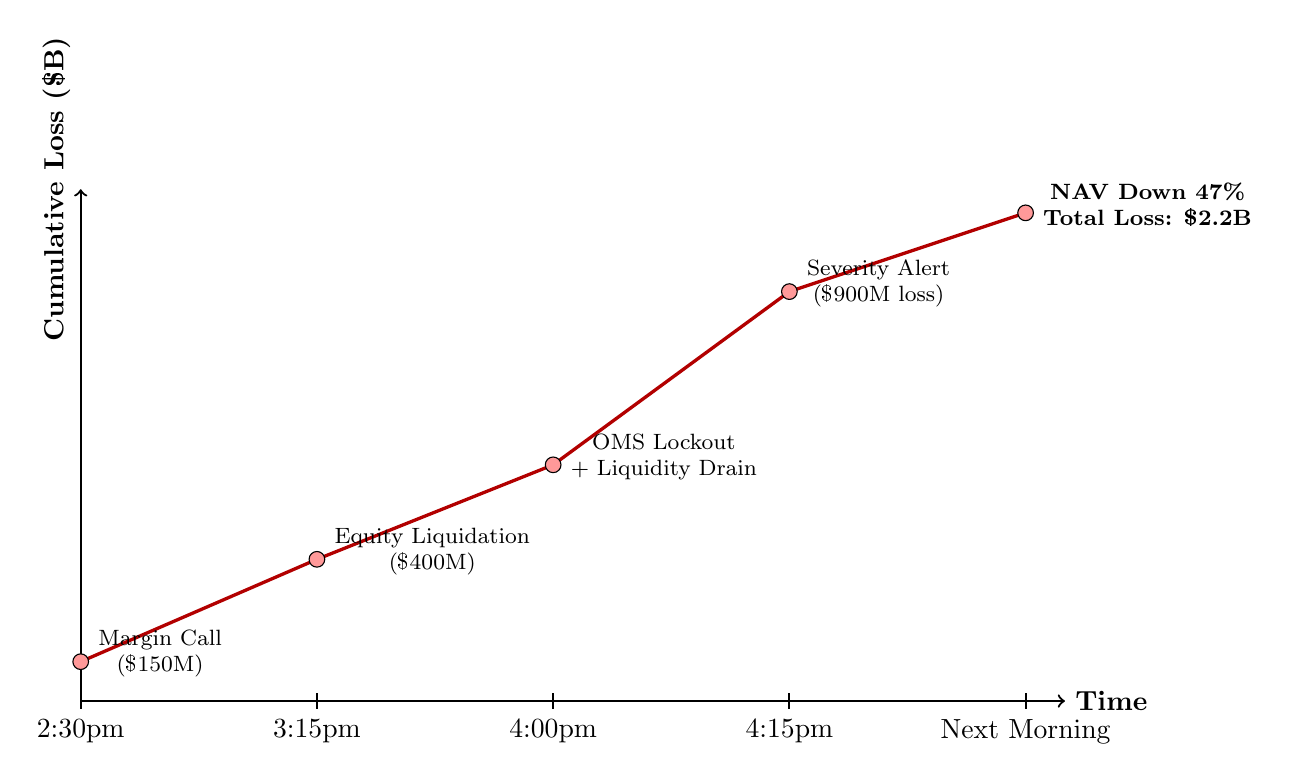
\begin{tikzpicture}[
    scale=1,
    axis/.style={thick, ->},
    event/.style={font=\footnotesize, align=center},
    loss/.style={circle, fill=red!40, draw=black, minimum size=4pt, inner sep=2pt}
  ]
  
  % Axes
  \draw[axis] (0,0) -- (12.5,0) node[right] {\textbf{Time}};
  \draw[axis] (0,0) -- (0,6.5) node[above, rotate=90] {\textbf{Cumulative Loss (\$B)}};
  
  % Time markers
  \foreach \x/\label in {
    0/2:30pm,
    3/3:15pm,
    6/4:00pm,
    9/4:15pm,
    12/Next Morning
  } {
    \draw[thick] (\x,0.1) -- (\x,-0.1) node[below] {\label};
  }
  
  % Loss line
  \draw[very thick, red!70!black]
    (0,0.5) 
    -- (3,1.8) 
    -- (6,3.0) 
    -- (9,5.2)
    -- (12,6.2);
  
  % Dots on line
  \node[loss] at (0,0.5) {};
  \node[loss] at (3,1.8) {};
  \node[loss] at (6,3.0) {};
  \node[loss] at (9,5.2) {};
  \node[loss] at (12,6.2) {};
  
  % Annotations
  \node[event, anchor=west] at (0.1,0.6) {Margin Call\\(\$150M)};
  \node[event, anchor=west] at (3.1,1.9) {Equity Liquidation\\(\$400M)};
  \node[event, anchor=west] at (6.1,3.1) {OMS Lockout\\+ Liquidity Drain};
  \node[event, anchor=west] at (9.1,5.3) {Severity Alert\\(\$900M loss)};
  \node[event, anchor=west] at (12.1,6.3) {\textbf{NAV Down 47\%}\\\textbf{Total Loss: \$2.2B}};
  
  \end{tikzpicture}
  \caption{Escalating Cumulative Loss: Arcadia's collapse unfolded in phases, each compounding the damage.}
\end{figure}

\medskip

By 10:12 a.m., their fund administrator still hadn’t updated the NAV file.  
Because no one knew what the portfolio was worth anymore.  
They only knew what was left to seize.

There was no warning. There was just automated triggers deep in the clearing system. The custodians didn’t call. 
The lawyers didn’t wait. The terms were predefined, and the math was cold. Arcadia's most liquid, high-quality 
assets were now gone: transferred without negotiation, in accordance with the agreements no one had re-read in years.

The machine learning system hadn’t caught the spiral because the model itself was \textbf{overfit}.

It had been trained on a world that was calm, segmented, and statistically clean. A world where \textit{oil 
prices and corporate bonds} danced to different rhythms. Where energy volatility was assumed to be independent 
from investment-grade credit.

It saw that — historically — these two variables didn’t move together. So it treated them like strangers at a 
party: in the same room, maybe, but not interacting.

But markets don’t behave like that under stress. \textbf{Under stress, independence collapses.} The wall 
between risk factors disappears. Everyone rushes for the same exits — at the same time.

\textbf{It’s like training a weather model on sunny days.}

You feed it years of calm skies and scattered clouds, and it learns that rain is rare and local. Then one 
day, a tropical storm forms offshore, but the model doesn’t recognize it. It doesn’t even have a word for 
``hurricane.''

So it keeps predicting a warm breeze... even when the roof blows off.

\medskip

\begin{PhilosophicalSidebar}{Systems Thinking and the Feedback Loop Trap}

  %\textbf{Origin: The Rise of Systems Thinking.}  
  In the mid-20th century, fields as diverse as biology, engineering, and military planning converged 
  around a shared insight: complex systems behave in ways that cannot be understood by examining individual 
  parts in isolation. This gave rise to \textit{cybernetics} — the study of feedback, control, and 
  communication in systems — pioneered by Norbert Wiener and later extended by figures like Jay Forrester 
  at MIT.

  \medskip
  
  %\textbf{Positive vs. Negative Feedback.}  
  Systems thinking distinguished between two types of feedback:  

  \medskip

  \begin{itemize}
    \item \textbf{Negative feedback} dampens volatility -- e.g., a thermostat turning off heat once a set 
    temperature is reached.  
    \item \textbf{Positive feedback} amplifies shocks —- e.g., margin calls triggering sales, which trigger 
    more margin calls.
  \end{itemize}

  \medskip
  
  %\textbf{Finance Discovers Feedback — Too Late.}  
  Despite its relevance, systems thinking arrived late to finance. Classical economic models favored 
  linearity, equilibrium, and independence. It wasn’t until repeated crises (from portfolio insurance in 
  1987, to LTCM in 1998, to the 2008 liquidity spiral) that feedback loops were recognized as systemic threats.

  \medskip
  
  %\textbf{The Arcadia Collapse: A Textbook Feedback Spiral.}  
  The model failed not because it lacked data, but because it lacked \textit{structure}. It treated 
  historical correlations as if they were laws. It did not treate them as emergent properties of a fragile, 
  interconnected system. Therefore, when oil crashed, Arcadia’s hedges amplified rather than absorbed losses. 
  Liquidity dried up.  The feedback loop ignited.  

  \medskip
  
  \textbf{And the model?}  
  It kept recommending ``rebalance.''
  As if you could rearrange deck chairs on a burning ship.
  
  \medskip

  \begin{center}
  \textit{In systems with positive feedback, stability is not the norm... it’s a temporary illusion.}
  \end{center}
  
\end{PhilosophicalSidebar}

\medskip


The real failure wasn’t complexity.  It was a blind trust in patterns that only held when nothing went wrong.

Investors weren’t asking questions. They were getting out. Pension funds. University endowments. Family offices. 
The ones who had praised the fund's ``adaptive AI risk engine'' in the good years now submitted terse, and 
one-line notices.

The lines on the redemption ledger didn’t come from fear. They came from strategy. Nobody wanted to be the 
last LP left holding the bag when the final markdown came.

Inside Arcadia, the illusion of control collapsed faster than the portfolio.

One PM tried to open a spreadsheet but stared blankly at the loading icon. Another whispered, 
``Do we even know what we own right now?'' A third walked out and didn’t come back.

The Irony? The AI dashboard was still green. \textit{But the lights in the office were turning off.}

\medskip

\begin{HistoricalSidebar}{Knight Capital: The \$440 Million Glitch}

  On August 1, 2012, Knight Capital Group, a major player in U.S. equities trading,  
  experienced a catastrophic software malfunction. A faulty deployment activated obsolete code,  
  triggering a dormant feature flag and causing the firm’s automated systems to execute errant trades at lightning speed.  
  Within 45 minutes, Knight had amassed unintended positions totaling approximately \$7 billion, resulting in a  
  loss of \$440 million.
  
  \medskip
  
  After an investigation, regulators found no willful misconduct. The engineers had followed protocol.  
  Sign-offs had been documented. Deployment processes had been technically satisfied.  
  There was no scapegoat. No intentional wrongdoing.  
  The disaster had emerged from a tragic convergence of overlooked legacy code and system complexity—  
  an error that might have happened to anyone.
  
  \medskip
  
  But it could have gone differently.
  
  \medskip
  
  Had the engineers skipped a sign-off, failed to document a test, or deviated from internal controls,  
  the finding could have shifted from “no fault” to negligence—or worse, willful misconduct.  
  And in securities law, there’s a thin, terrifying line:  
  Most corporate indemnification protects you from mistakes.  
  But it stops short at two critical points:  
  \textbf{willful misconduct} and \textbf{gross negligence}.
  
  \medskip
  
  In highly regulated industries, you don’t need to commit fraud to face prosecution.  
  You only need to fail to do enough.
  
  \medskip
  
  In the wake of the collapse, new regulations were enacted. Additional verification steps mandated.  
  Audit trails hardened. Controls tightened.  
  But the deeper lesson remained unsettling:  
 
  \begin{quote}
  Sometimes, even with due diligence, the system can still break.  
  And if you’re standing too close to the fault line when it does,  
  there’s no guarantee the legal shield will hold.
  \end{quote}
  
\end{HistoricalSidebar}


\subsubsection{Narrative \& Structure}

\begin{itemize}
  \item Did the section open with the appropriate sense of escalation or drama?
  \item Was the pacing effective through the margin cascade?
  \item Was the blending of technical, emotional, and narrative stakes successful?
  \item Were there moments that felt overly explained or underdeveloped?
\end{itemize}

\subsubsection{Technical Clarity}

\begin{itemize}
  \item Was the ISDA figure clear and helpful? Would a reader unfamiliar with derivatives follow it?
  \item Did the liquidation steps make sense chronologically and financially?
  \item Were terms like \texttt{Schedule A}, \texttt{CSA}, and \texttt{variation margin} clearly contextualized?
  \item Is there any technical point where clarification or visual simplification might help?
\end{itemize}

\subsubsection{Emotional Impact}

\begin{itemize}
  \item Did the mood land — the silence, the spiral, the loss of control?
  \item Was the comparison to '08 or the weather model metaphor emotionally effective or distracting?
  \item Were the comic panels tonally consistent with the gravity of the scene?
  \item Did the pacing between figures, text, and sidebars heighten or dilute the impact?
\end{itemize}

\subsubsection{Sidebar Utility}

\begin{itemize}
  \item Did the \textbf{HistoricalSidebar} on NAV help frame the stakes?
  \item Did the \textbf{TechnicalSidebar} on margin and collateral explain the mechanics or interrupt the flow?
  \item Did the \textbf{PhilosophicalSidebar} on feedback loops clarify the model's failure mode?
  \item Were the sidebars well-integrated or too heavy for the pacing?
\end{itemize}

\subsubsection{Thematic Depth}

\begin{itemize}
  \item Does the section deepen the theme of algorithmic fragility under stress?
  \item Does it convincingly show how technical logic can become structural risk?
  \item Are the comparisons (Knight Capital, margin hierarchy, systems theory) additive?
  \item What more could be drawn out from the collapse?
\end{itemize}



\subsection{The Audit}

When the dust settled, the auditors arrived.
The auditors did not arrive with alarms or outrage. They arrived with clipboards, spreadsheets, and institutional detachment.
They didn’t need to ask who was responsible. The signatures were already timestamped. The logs were immutable. 
The collapse was self-documenting.

Then came the regulators.
They were slower, but hungrier.
They didn’t come to fix the system. They came to write the story... and to make sure someone’s name filled 
the footnotes of failure. They asked questions that sounded simple but weren’t.

They started with the logs.
Timestamps. Code updates. Deployment notes.
Every action left a footprint — and footprints always lead somewhere.

They followed the trail to the model.
The one that was supposed to catch the risk.
But it didn’t.
It focused on the wrong signals, at the wrong time, in the wrong kind of market.

Then they looked at how that model got out there.
A rushed launch, pushed out two weeks early.
A freeze on changes that nobody stuck to.
A last-minute patch that skipped review because “we had to move fast.”

And finally, they traced it back to the moment it became official.
The sign-off.
The digital “okay” that made it real.
The click that turned a line of code into a real-world failure.

And the sign-off?  \textbf{David’s initials.}

Three letters in the lower right corner of the commit approval screen.
A routine click, made after a long day, probably during a Zoom call.
No malicious intent. No recklessness.
Just the ordinary negligence of someone who believed the system was stable.
Because it always had been.  Until it wasn’t.

\medskip

\begin{HistoricalSidebar}{Auditors vs. Regulators — Two Tribes of Postmortem Power}

  When financial systems fail, two professional species arrive: \textbf{auditors} and \textbf{regulators}. 
  Both investigate. Both ask questions. But their mandates — and temperaments — diverge in subtle, consequential ways.

  \medskip
  
  \textbf{Auditors} are internal or contracted examiners. Their job is to verify compliance with stated policies, 
  reconcile transactions, and ensure that procedures — even flawed ones — were followed. They don’t ask whether a 
  rule made sense. They ask whether it was followed and documented.

  \medskip
  
  In the 2001 Enron collapse, Arthur Andersen’s audit teams had documented procedures — but failed to challenge 
  the legitimacy of off-balance-sheet structures. They checked the math. They missed the meaning.

  \medskip
  
  \textbf{Regulators}, on the other hand, arrive on behalf of public institutions. Their mission is broader: 
  assess systemic risk, uncover governance failures, and assign accountability. While auditors scrutinize evidence, 
  regulators write the narrative. Where auditors measure, regulators interpret.

  \medskip
  
  After the 2008 crisis, agencies like the SEC, CFTC, and Financial Crisis Inquiry Commission sought more than numbers: 
  they sought names. Lehman’s liquidity “death spiral,” AIG’s collateral triggers, and Citi’s CDO masking all became 
  regulatory foci not just because rules were broken, but because stories were buried.

  \medskip
  
  In Aurora’s case, the auditors came first. They brought spreadsheets.  
  The regulators came later. They brought subtext.
  
\end{HistoricalSidebar}

\medskip




``Who approved the leverage?'' asked the Senior Forensic Analyst from the SEC, eyes steady over rimless glasses.

David sat with his hands folded, palms damp. ``The decision to raise the exposure cap came from the portfolio team. 
I wasn’t involved in that approval.''

The analyst didn’t nod. He just blinked once. ``But you provided the risk assessment, correct?''

David hesitated. ``I prepared the system output. Yes.''

``Specifically the version dated three days before the exposure increase?''

``Yes.''

The analyst flipped through a binder, stopping at a page with highlighted sections. ``According to this, the model 
flagged an increase in cross-asset volatility. Why was that column excluded in the final risk memo sent to 
Investment Oversight?''

David felt the heat rise in his neck. ``We were still calibrating the signal. At that point, it had high sensitivity 
and was generating noise—false positives.''

``And who made the decision to suppress it?''

David paused. ``Technically, I did.''

``Why?''

He swallowed. ``Because I didn’t want it to distract from the broader findings. The rest of the model showed 
acceptable thresholds.''

The analyst looked up. ``Acceptable under what assumptions?''

``Under calm regime behavior. Which, at the time—''

``—was already breaking down in commodity markets,'' the analyst interrupted gently. ``You removed the only 
indicator showing early instability. Why?''

David shifted in his seat. ``We thought it was a blip. Noise.''

``Did you note that in the report?''

``No. It didn’t seem material at the time.''

``Yet it was material enough to suppress?''

The room fell quiet.

The analyst tapped his pen once on the table. ``So, when Investment Oversight pushed the leverage increase, 
they were acting under the impression that all volatility indicators were neutral.''

David didn’t answer.

``And the one flag that wasn’t neutral — the one warning sign — was missing because you thought it might cause confusion.''

David looked down. ``I didn’t mean to mislead anyone.''

``Intent isn't the question,'' the analyst said. ``The question is whether your report enabled a decision that 
should never have been made.''

Another pause. Then:

``Mr. Morales,'' he continued, ``your name appears on the approval workflow. Not as decision-maker, but as 
validator. Your initials are here—right under the model output. Do you dispute that?''

David stared at the page.

``No,'' he said quietly. ``I don’t dispute that.''

``Thank you,'' the analyst said, and closed the binder with a soft click.

``That will do for now.''

\medskip

\begin{HistoricalSidebar}{The SEC and the Theater of Responsibility}

  Founded in the wake of the 1929 crash, the U.S. Securities and Exchange Commission (SEC) was designed as both 
  watchdog and confessor. It was designed to be part enforcement arm, and part national conscience for financial markets.

  \medskip
  
  Its mandate is simple: protect investors, ensure fair markets, and hold those accountable who threaten either. 
  But the execution is rarely so clean.

  \medskip
  
  In scenarios like David’s, the SEC doesn't storm the gates with sirens. It arrives in tailored suits and 
  calibrated language, interested less in guilt than in \textit{who signed what, and when}. It reconstructs the internal 
  machinery: approval chains, suppressed signals, reporting thresholds — all to trace how a decision came to look inevitable.

  \medskip
  
  By the time the SEC enters the room, the damage is already done. Its job is to illuminate the moment it became 
  irreversible, to identify who, and hold the flashlight on them.
  
\end{HistoricalSidebar}

\medskip

``Why wasn’t the risk flagged?'' asked the Deputy Director of Risk Oversight from the Office of Systemic Risk.

His voice was calm, but he was already circling the failure — not of markets, but of \textit{detection}.

David took a beat. ``It depends which risk you’re referring to.''

``The synthetic credit tranche that ruptured three liquidity pools in under ninety minutes.''

David exhaled slowly. ``That product was flagged — in internal simulations. We just didn’t escalate it.''

``Why not?''

``The model showed instability only in certain stress-paths. And only when run at the 95th percentile sensitivity. Leadership considered that noise.''

``Did you?''

David hesitated. ``I thought it needed more time. The signal hadn’t stabilized.''

``And in the meantime, the exposure increased by 31\%.''

``I wasn’t in charge of allocations.''

``No,'' the Deputy Director said. ``But your report was cited as justification in the allocation memo.''

David blinked. ``I wasn’t aware of that.''

``Page 4, footnote 2. They reference your summary of model results and cite the volatility corridor as ‘within tolerance.’ Was it?''

David looked down. ``Only if you exclude derivative spillover effects. Which I hadn’t tested yet.''

``So you signed off on a model summary that didn’t include derivatives — even though the product in question was synthetic credit?''

``We were on a compressed timeline. There was pressure to deliver a greenlight framework by end-of-quarter.''

``From whom?''

``Multiple stakeholders.''

``Can you name them?''

``I'd prefer not to speculate.''

``You don’t need to speculate, Mr. Morales. You need to remember.''

A silence stretched — not hostile, but surgical.

``Let me put it another way,'' the Deputy Director said, folding his hands. ``You were responsible for identifying unstable pathways in Aurora’s credit engine. And yet, the most dangerous path — the one that actually unfolded — wasn’t flagged, wasn’t communicated, and wasn’t contained.''

``The model wasn’t broken,'' David said quietly. ``It just wasn’t finished.''

The Director nodded slowly. ``Neither was the crisis.''

``Thank you,'' he said, closing his folder. ``That will be all for now.''

\medskip

\begin{HistoricalSidebar}{The Office of Systemic Risk --- After the Crash, the Cartographer}

  The \textbf{Office of Systemic Risk}, operating under the Financial Stability Oversight Council (FSOC), 
  was created by the Dodd–Frank Act in 2010. It is not a market regulator, but a mapmaker of collapse.

  \medskip
  
  Its mandate wasn’t to monitor firms individually, but to identify threats that emerge when interlocking 
  systems --- funds, models, margin calls, and political pressures --- align catastrophically. In other words: 
  not \textit{who} failed, but \textit{how} the system was already wired to fail.

  \medskip
  
  In cases like Aurora, the Office doesn’t arrive looking for fraud. It arrives looking for fragility that 
  was normalized — risks that were technically visible, but socially invisible. Often, the most damaging 
  decisions were made with clean hands and plausible models.

  \medskip
  
  The Office’s investigators specialize in tracing these moments: where a suppressed flag or a downgraded 
  simulation quietly mutated into systemic exposure. Their job isn’t to prevent the last crash. It’s to 
  draw the blueprint for the next one, and to ask why no one sounded the alarm when the walls were 
  already shaking.
  
\end{HistoricalSidebar}

\medskip


``Where’s the board memo?'' asked the man in the dark suit — Special Counsel for the Congressional Subcommittee 
on Financial Accountability. He spoke plainly, but each word felt like it had been cleared with legal counsel.

David looked down at the folder in front of him. ``Which memo, exactly?''

``The one documenting leadership’s awareness of the leverage adjustment and cross-product exposure. The one that 
should’ve gone to the Risk and Audit Committee in Q2. We’ve reviewed the board packets. It’s not there.''

David cleared his throat. ``If it wasn’t escalated, that would’ve been Compliance’s responsibility.''

The counsel nodded once. ``So you didn’t draft a briefing note?''

``No formal memo, no. We discussed elements of it in working groups.''

``Any minutes from those meetings?''

``Possibly. Not all sessions were minuted.''

``Were any slides presented to executive leadership?''

``There were slides,'' David said. ``But they were high-level.''

``How high-level?''

``Portfolio allocation bands. General trends. Scenario ranges.''

``Any mention of the synthetic tranche correlation drift?''

David hesitated. ``Not explicitly, no.''

The counsel glanced down at a binder. ``Your team internally referred to that drift as `uncontained contagion 
velocity’ in a Slack thread dated April 17th. Would you say that rises to the level of board visibility?''

David blinked. ``That was informal language.''

``So the board received a sanitized version?''

``They received a \textit{strategic} summary,'' David said carefully.

``Without the risks.''

``Without the emerging anomalies,'' he corrected.

``And who decided those anomalies didn’t merit inclusion?''

``That would have been a judgment call across multiple leads.''

``But your name is listed as the document owner on the draft outline. Yes?''

David didn’t answer.

The counsel didn’t press — not directly.

``Mr. Morales, when boards are kept in the dark, we investigate whether it was by accident or by design. Right now, 
it looks like your team filtered the light. That’s not a modeling issue. That’s governance.''

He closed the folder.

``And the next question will be: who gave permission... and who gave cover.''

\medskip

\begin{HistoricalSidebar}{The Congressional Subcommittee on Financial Accountability}

  The \textbf{Congressional Subcommittee on Financial Accountability} is less a financial authority and more a political 
  lens — trained on moments when markets fail and someone, somewhere, must be made to answer.

  \medskip
  
  Historically activated after high-visibility collapses --- Enron (2001), Lehman Brothers (2008), Archegos (2021) --- the 
  Subcommittee is tasked with tracing breakdowns in oversight, disclosure, and board governance. Its focus isn’t technical 
  modeling or trading algorithms; it’s \textit{who knew what, when}, and why warnings were buried, softened, or ignored.

  \medskip
  
  Unlike regulatory bodies such as the SEC or FSOC, which prioritize structural risk, the Subcommittee pursues political 
  and ethical accountability. It doesn’t ask if the system failed. It asks whether people in positions of fiduciary trust 
  failed to act.

  \medskip
  
  In hearings, terms like ``strategic ambiguity,'' ``sanitized summaries,'' and ``decision path opacity'' become signals 
  of willful negligence. In this theater, plausible deniability often reads as intent.

  \medskip
  
  The result may not be criminal indictment. Howeverr, reputational collapse begins here.
  
\end{HistoricalSidebar}

\medskip


\begin{TechnicalSidebar}{Due Diligence, Delegation, and the Architecture of Deniability}

  David Morales believed he was protected.  
  Aurora wasn’t the contracting party. The deployment was Centauri’s. The Delaware LLC offered corporate insulation.  
  But legal shields only hold when due diligence is intact.
  
  \medskip
  
  In regulatory doctrine, \textbf{limited liability} and \textbf{role separation} are not get-out-of-jail-free cards —  
  they are privileges that assume \textit{reasonable care within one's domain}.

  \medskip
  
  Morales, as technical validator, was expected to:

  \medskip
  
  \begin{itemize}
    \item Identify and escalate model anomalies,
    \item Document suppressed signals or internal uncertainty,
    \item Ensure executive briefings were technically truthful — not just politically convenient.
  \end{itemize}

  \medskip
  
  He failed in each.  
  He didn’t lie. He didn’t conspire.  
  But he clicked “approve” on a model he knew was incomplete — and that single act converted risk into exposure.
  
  \medskip
  
  \textbf{Michael Hart}, by contrast, had engineered something else entirely:  
  \textbf{plausible deniability by design}.

  \medskip
  
  Centauri owned the deployment.  
  Aurora owned the code — but not the contract.  
  Hart held no formal role in the decision tree. He was the architect, not the executor.
  
  \medskip
  
  He didn’t need to sign anything.  
  He just needed to stage the room, whisper the timelines, and let someone else do the nodding.
  
  \medskip
  
  To a regulator, Morales was the approval trail.  
  To a court, Hart was just an advisor.  
  This was the genius of the structure: \textbf{accountability flowed downhill, but control flowed up.}
  
\end{TechnicalSidebar}

\subsection{Editor Questions for ``The Audit''}

This section marks the forensic pivot of the story — where narrative gives way to inquiry, and character gives way to accountability. It shifts the emotional weight from seduction to responsibility, asking the reader to confront systemic failure through the lens of human fallibility. These questions aim to explore the resonance, structure, and clarity of this shift.

\subsubsection{Narrative \& Structure}

\begin{itemize}
  \item Did the chapter maintain momentum despite its procedural tone?
  \item Did the transition from narration into interrogation feel fluid or jarring?
  \item Was the layering of events — audit, SEC, systemic risk, Congressional hearing — clear and well-paced?
\end{itemize}

\subsubsection{Psychological \& Emotional Realism}

\begin{itemize}
  \item Did David's emotional responses feel authentic under pressure?
  \item Were the silences and hesitations believable moments of human stress — or overplayed?
  \item Did the language make you feel sympathy, frustration, or distance from him?
\end{itemize}

\subsubsection{Thematic Clarity}

\begin{itemize}
  \item What do you think this section is ultimately about: accountability, negligence, systems collapse — or something else?
  \item Did the narrative succeed in balancing personal failure with institutional failure?
  \item Was the theme of “small actions with large consequences” effectively conveyed?
\end{itemize}

\subsubsection{Ethical and Emotional Tension}

\begin{itemize}
  \item Did you feel implicated, angered, or numb by David’s role in the collapse?
  \item Were the interrogations fair? Or did they feel more like blame-seeking than truth-seeking?
  \item Did the chapter evoke any personal reflections on workplace responsibility or complicity?
\end{itemize}

\subsubsection{Sidebars \& Contextual Frames}

\begin{itemize}
  \item Did the historical sidebars (Auditors vs. Regulators, SEC, FSOC, Congressional Oversight) enhance your understanding of the stakes?
  \item Were any sidebars redundant or overly didactic?
  \item Would you prefer these sidebars to be more tightly woven into the dialogue or narration?
\end{itemize}

\subsubsection{Language \& Style}

\begin{itemize}
  \item Did the procedural tone feel sharp and immersive, or dry and technical?
  \item Were there lines that helped break the legal monotony with emotional weight or dramatic tension?
  \item Did the use of repeated structures (“the click,” “the sign-off,” “the folder”) help build tension or feel formulaic?
\end{itemize}

\subsubsection{Optional: Reader Reflection}

\begin{itemize}
  \item If you were David, what would you have done differently — if anything?
  \item Who did you feel had more control: David, Hart, the regulators, or the system itself?
  \item What line, moment, or exchange stayed with you most after reading?
\end{itemize}








\subsection{The Hearings}


And then the subpoenas.  
Each one a bullet with a return address.  
Not everyone got one. Just enough to split the room.


The investigation was clinical, and methodical.  
There were no accusations. No raised voices.  
Just quiet meetings behind closed doors,  
and inboxes filling with calendar invites marked “Confidential.”

\medskip

\begin{HistoricalSidebar}{Subpoenas --- Paper Bullets with a Return Address}

  \textbf{Subpoena} comes from the Latin \textit{sub poena} — ``under penalty.'' It began as a writ in English 
  common law, compelling individuals to testify or produce documents. By the 15th century, it had become a 
  formal mechanism of legal extraction — not to accuse, but to compel.

  \medskip

  In modern investigations, subpoenas don’t arrive with sirens. They arrive in email threads, compliance inboxes, 
  and quietly worded calendar invites. They don’t raise voices. They split rooms.

  \medskip

  Issued selectively, they create informational asymmetry. Early recipients wonder if they’re targets or witnesses. 
  Later recipients assume someone already talked. No one says much — because now, everything is being recorded.

  \medskip

  Subpoenas don’t tell a story. They demand one. They initiate a narrative transition — from ambiguity to deposition, 
  from Slack to sworn testimony. From plausible deniability to forensic inevitability.
  
\end{HistoricalSidebar}

\medskip

The Financial Stability Oversight Council had been silent—until it wasn’t.
After the volatility cascade triggered margin calls across three major clearinghouses, cross-institutional exposure became a national concern.
Funds were gated. Credit lines frozen. Secondary markets evaporated overnight.
What began as a mispriced tranche had metastasized into a full-spectrum liquidity crisis, touching everything from pension systems to municipal bonds.

Now the FSOC wasn’t there to fix it.
They were there to reconstruct it—step by step, decision by decision.

The Deputy Director sat at the head of the table, flipping through a printout of Risk Weekly.
Without looking up, he asked:
“Who approved the tranche acceleration?”

Rishi Agarwal, Portfolio Lead, didn’t hesitate. The phrasing had been practiced.
“It was flagged neutral in Risk Weekly,” he said.

A pause.

“Who signed off on Risk Weekly?”

Rishi’s voice was lower now. Less certain.
“David Morales.”

And that was why they were in the room: not to speculate, but to follow the signatures.

\medskip

\begin{TechnicalSidebar}{Tranche Acceleration — When Slices Become Triggers}

  A \textbf{tranche} is a structured slice of a financial product — typically a synthetic or securitized 
  instrument — used to allocate risk and return across different investor classes. Senior tranches receive 
  payments first and absorb losses last, while equity tranches sit at the bottom of the stack, exposed to 
  first loss.

  \medskip

  \textbf{Tranche acceleration} is a contractual mechanism that forces early payout, repricing, or 
  liquidation of one or more tranches when certain thresholds are breached — often tied to volatility, credit 
  spread drift, or model-based metrics.

  \medskip
  
  While these clauses are designed to protect senior tranches, they can trigger rapid portfolio reconfiguration. 
  The result is often a forced liquidation cascade, especially when leverage is high or liquidity is thin. 
  Acceleration transforms a slow deterioration into a sudden collapse.

  \medskip
  
  A defining example came in 2007, when two Bear Stearns hedge funds — heavily exposed to subprime mortgage-backed 
  CDOs — faced mounting margin calls. As junior tranches deteriorated, acceleration clauses were triggered across 
  multiple instruments. The resulting fire sale flooded the market with distressed assets, collapsing prices and 
  evaporating confidence. Bear Stearns was forced to inject \$3.2 billion in emergency funding, but the funds 
  imploded anyway — a prelude to the 2008 crisis.

  \medskip
  
  In Aurora’s case, the decision to neutral-flag a potential acceleration scenario may have appeared conservative 
  — but history shows how quickly “non-critical” can become irreversible.
  
\end{TechnicalSidebar}

\medskip

\begin{figure}[H]
  \centering
  \begin{tikzpicture}[font=\small, every node/.style={align=center}]
  
    % Tranche boxes (stacked top to bottom)
    \node[draw, fill=gray!30, minimum width=4cm, minimum height=1cm] (senior) at (0,3) {\textbf{Senior Tranche}\\\scriptsize Paid first, losses last};
    \node[draw, fill=orange!30, minimum width=4cm, minimum height=1cm, below=0cm of senior] (mezz) {\textbf{Mezzanine Tranche}\\\scriptsize Middle risk-return};
    \node[draw, fill=red!30, minimum width=4cm, minimum height=1cm, below=0cm of mezz] (equity) {\textbf{Equity Tranche}\\\scriptsize First loss absorbed here};
  
    % Labels on left
    \node[anchor=east] at (-2.7,3) {\footnotesize Lowest Risk};
    \node[anchor=east] at (-2.7,1) {\footnotesize Moderate Risk};
    \node[anchor=east] at (-2.7,-1) {\footnotesize Highest Risk};
  
    % Trigger point arrow (credit deterioration)
    \draw[->, thick, red] (-3.5,0) -- (-0.1,0) node[midway, above, sloped] {\scriptsize Subprime collapse, volatility spike};
  
    % Acceleration arrow across structure
    \draw[->, thick, orange, dashed] (0.2,2.9) -- ++(3.2, -2.8) node[midway, right, font=\scriptsize, align=left] {Acceleration clause\\triggers payout or\\forced liquidation};
  
    % Liquidation arrow
    \draw[->, thick, red] (equity.south) -- ++(0,-1.5) node[midway, right] {\scriptsize Fire sale / price collapse};
  
    % Surrounding caption
    \node[align=center, font=\small, text width=11cm, below=2.8cm of equity] {
      \textbf{Tranche acceleration} turns gradual deterioration into rapid collapse.\\
      Senior tranches are protected by structure — but once acceleration is triggered,\\
      the full stack can unravel via forced selling, especially under stress.
    };
  
  \end{tikzpicture}
  \caption{Tranche structure with acceleration dynamics. When lower tranches deteriorate, acceleration clauses can liquidate the stack, triggering contagion.}
  \end{figure}

\medskip

The hearings weren’t supposed to happen—at least not this soon.
But after the leverage ratio disclosures leaked to the press, and equity markets shed 6% in a single afternoon, congressional pressure moved from possibility to inevitability.

This wasn’t just an inquiry into capital structure.
It was an inquiry into the *story* of the capital structure—
What was said. What was shown. And what was strategically left unsaid.

At the center of it sat Janine Cole, Head of Capital Strategy.
She wasn’t on trial. Not formally.
But she had been in the room.
She had seen the deck.
And now she was being asked to name the omissions.

The Special Counsel leaned forward, voice flat:
“Was leverage discussed in the Q2 oversight call?”

Janine nodded, then qualified:
“Only after David’s slides were reviewed.”

A pause. Then the follow-up:
“Who built the slides?”

Her reply was quiet, procedural.
“David did. Hart approved the framing.”

The committee didn’t react. They didn’t need to.
The point wasn’t the answer.
The point was the sequence.



\medskip

\begin{TechnicalSidebar}{Oversight Calls — Rituals of Supervision, or Theaters of Compliance?}

  \textbf{Oversight calls} are recurring governance checkpoints in which senior stakeholders — typically board 
  members, risk officers, capital managers, and legal observers — are briefed on material developments. These 
  calls are meant to ensure that large financial institutions surface emerging risks and maintain a documented 
  trail of responsible supervision.

  \medskip
  
  In theory, oversight calls act as early-warning systems — surfacing anomalies, validating assumptions, and 
  adjusting exposure. In practice, they are often sanitized. Framing is everything.

  \medskip
  
  Slide decks, discussion pacing, and choice of which risks to highlight — and which to label ``under review'' — 
  can dramatically alter perception. What’s left unsaid often carries more consequence than what’s disclosed.

  \medskip
  
  After the 2008 crisis, multiple Senate hearings revealed that oversight calls at institutions like Lehman 
  Brothers and AIG did technically occur — but were functionally meaningless. They were either built around 
  already-approved narratives, or structured to minimize alarms. Formal governance was preserved; actual 
  intervention was not.

  \medskip
  
  In Aurora’s case, leverage was technically discussed. But the framing — delivered through David’s slides 
  and shaped by Hart’s cues — ensured that the risk appeared contained, optional, and well within tolerances. 
  It was theater. And like all good theater, it left the audience reassured.
  
\end{TechnicalSidebar}


\medskip

“Did anyone question the model sensitivity thresholds?”
The SEC analyst’s voice was clinical, almost bored.
But everyone in the room knew the weight behind the question.

Linda Chow, Quantitative Analyst, kept her eyes forward.
“David said noise filtering was standard,” she replied.

That phrase—noise filtering—was at the heart of it.

By the time the SEC stepped in, the case had already shifted.
It wasn’t just a model failure anymore.
It was a disclosure issue.

The predictive engine that underpinned the entire risk platform had been suppressing volatility signals for over six quarters.
Not by accident. By design.
Spikes were smoothed. Deviations flattened.
What should have triggered escalation was quietly filed under “non-material variance.”

The analyst pressed on:
“Did you agree with that?”

Linda didn’t look up.
“It didn’t seem optional.”

She hadn’t built the system. But she had run the simulations.
And she knew exactly what happened to people who flagged false positives—especially if they made a pattern of it.

Now, the investigation wasn’t just about thresholds or tuning parameters.
It was about the cultural physics of silence—
and how models can inherit the blind spots of the people who fear asking the wrong questions.


\medskip

\begin{TechnicalSidebar}{Sensitivity Thresholds — Where Judgment Becomes Justification}

  In quantitative modeling, a \textbf{sensitivity threshold} defines how much a model’s output is allowed 
  to change in response to shifts in its inputs — like volatility, interest rates, credit spreads, or market 
  liquidity indicators. It is a tuning dial for how reactive (or inert) the model appears.

  \medskip
  
  Thresholds are often used to suppress ``noise'' — minor fluctuations not considered materially significant. 
  But the line between noise and signal is not a scientific fact. It’s a judgment call. And that judgment, 
  once embedded in code or policy, becomes invisible to downstream decision-makers.

  \medskip
  
  Historically, sensitivity thresholds have played silent but pivotal roles in financial collapses. In the 
  lead-up to the 2008 crisis, Value-at-Risk (VaR) models at firms like Lehman and Merrill Lynch used smoothing 
  techniques to underplay tail risk. These techniques were technically valid — but strategically convenient.

  \medskip
  
  A similar case emerged in 2012 during the JPMorgan ``London Whale'' incident. Internal models used 
  understated volatility estimates to lower risk flags — until losses ballooned past \$6 billion. Again, 
  thresholds hadn’t broken rules. They’d merely been tuned.

  \medskip
  
  In Aurora’s case, David’s designation of noise filtering as ``standard'' functioned as a rhetorical sleight 
  of hand. It implied consensus. It implied safety. But for Linda — and others — the decision was framed as a 
  default, not a debate. And once a threshold is normalized, its danger lies not in what it hides, but in 
  how little scrutiny it attracts.
  
\end{TechnicalSidebar}
  

\medskip
\begin{figure}[H]
  \centering
  \begin{tikzpicture}[font=\small, node distance=1cm and 2cm]
  
    % DIAL metaphor
    \node[draw, fill=blue!10, circle, minimum size=2.5cm, align=center] (dial) 
      {\textbf{Sensitivity Threshold}};
    \node[above=0.3cm of dial, font=\bfseries] {Model Tuning};
  
    % Input stream (signal/noise)
    \draw[->, thick] (-5,0) -- (dial.west) node[midway, above] {\scriptsize Market Inputs (volatility, spreads, etc.)};
  
    % Filtered output path
    \draw[->, thick] (dial.east) -- (2.5,0) node[midway, above] {\scriptsize Filtered Output};
  
    % Signal chart (expected vs filtered)
    \draw[thick, ->] (5.2, -0.5) -- ++(4.3,0) node[right] {\small Time};
    \draw[thick, ->] (5.2, -0.5) -- ++(0,2) node[above] {\small Risk Signal};
  
    % Draw true signal curve (dashed)
    \draw[red, thick, densely dashed, domain=5.3:9.2, samples=100] 
      plot(\x, {0.3*sin(3*\x r)+1});
  
    % Draw filtered (thresholded) signal
    \draw[blue, thick, domain=5.3:9.2, samples=100, variable=\x]
      plot(\x, {max(0.3*sin(3*\x r)+1-0.15,0.4)});
  
    \node[red, font=\scriptsize] at (7.2,1.6) {True Signal};
    \node[blue, font=\scriptsize] at (7.4,0.65) {Thresholded Output};
  
    % Side note
    \node[align=left, text width=5cm, right=1.5cm of dial, anchor=west, font=\small] (note) {
      \textbf{Suppressed risk signals}
      Threshold tuning may hide minor fluctuations — 
      but can also mute early warnings before collapse.
    };
  
    % Consequence box
    \node[draw, fill=red!20, rounded corners, minimum width=3.8cm, below=1.2cm of dial, align=center] (hidden)
      {Muted Alerts\\\small (No alarms triggered)};
    \draw[->, thick] (dial.south) -- (hidden.north);
  
    \node[draw, fill=red!40, rounded corners, minimum width=3.8cm, below=1.2cm of hidden, align=center] (rupture)
      {Delayed Response\\\small (Losses accumulate)};
    \draw[->, thick] (hidden.south) -- (rupture.north);
  
    % Label
    \node[below=1.2cm of rupture, font=\small\itshape] {
      The problem isn’t just what the model misses —
      it’s how confidently it misses it.
    };
  
  \end{tikzpicture}
  \caption{A sensitivity threshold suppresses minor risk signals. But when judgment becomes default, early warnings are filtered out — not because the model is broken, but because it’s tuned to be silent.}
  \end{figure}
  

  \medskip

“Who pulled the derivative drift chart from the board packet?”
The question landed without ceremony, just a line read aloud by Audit Counsel as if it were a formality.
But everyone at the table knew it wasn’t.

Marcus Bell, Governance Liaison, cleared his throat.
“It was in the draft. David removed it before submission.”

That chart—showing sustained drift in the derivatives desk’s internal pricing—was supposed to be on slide 14.
It wasn’t.

Two weeks before the board convened, it had quietly disappeared.
In its place, a cleaner narrative took shape.
At the same time, a new line made its way into regulatory filings:
Exposure ceilings remain within tolerance.
Now, in hindsight, that language didn’t look justified.
It looked planted.

The Regulatory Liaison from the Office of Systemic Risk turned to the next witness.
“Who certified exposure ceilings were within tolerance?”

Amira Khan, VP of Risk Ops, responded evenly.
“That language came from David’s team.”

A pause.

“Did he write it?”

“He presented it,” she said.
Then added, almost as an afterthought:
“Hart sat in, but said nothing.”

The internal review was no longer about oversight failure.
It was about narrative control.
Who shaped the version of reality that made it to the boardroom—
and who let it through.

\medskip

\begin{TechnicalSidebar}{The Derivative Drift Chart — When Models Wander into Trouble}

  A \textbf{derivative drift chart} is a diagnostic tool used to monitor how financial derivatives 
  — especially those priced by internal models — deviate over time from observable market behavior. 
  It tracks the ``drift'' between model-predicted prices and actual market valuations, surfacing 
  anomalies in calibration, volatility assumptions, or counterparty inputs.

  \medskip
  
  Minor drift is expected. But persistent or accelerating drift often signals that a model is 
  losing touch with reality — either because of external shocks (regime shifts, illiquidity) or 
  internal failure (poor inputs, stale data, misaligned risk factors).

  \medskip
  
  The chart is visual — and that's what makes it dangerous to hide. Unlike a footnote or line item, 
  it shows the divergence at a glance. A spike in drift doesn’t need translation. It needs explanation.

  \medskip
  
  In the aftermath of the Long-Term Capital Management (LTCM) collapse in 1998, internal drift diagnostics 
  had shown warning signs for weeks, but were buried in appendices. A similar case occurred in the 2018 
  blow-up of short-volatility products (e.g., XIV), where delta drift and gamma exposure were downplayed 
  in risk packets, despite internal visualizations showing growing instability.

  \medskip
  
  In Aurora’s case, the chart existed — briefly. It was in the board packet draft, flagged for discussion. 
  And then it wasn’t. When Marcus Bell confirmed its removal, and Amira Khan noted Hart’s silent presence 
  during its exclusion, it was clear: omission wasn’t an oversight.

  \medskip
  
  It was strategy.
  
\end{TechnicalSidebar}

\medskip

“Why wasn’t the volatility cascade escalated?”
The Oversight Investigator didn’t shout. He didn’t need to. The question had been sitting at the center of every 
closed-door session since the collapse.

Nikhil Rao, Head of Compliance Reporting, answered with the kind of practiced restraint that only made the silence louder.
“We assumed David had.”

That assumption had become the architecture of the failure.

By the time the cascade hit, hedging correlations had snapped, liquidity had vanished, and the aftershocks were tearing 
through sovereign swaps, structured notes, and retail derivatives alike.
Internal systems had fired alerts.
Logs showed escalation triggers.
But nothing made it out of the building.

The Investigator pressed:
“Did you ask him?”

Nikhil’s tone didn’t change, but his meaning did.
“You didn’t question David back then. Not if you wanted to stay.”

The Treasury Working Group had been tasked with one goal:
identify why no one pulled the brake
Now they were uncovering the answer—one conversation at a time.

Later, in a separate hearing, the focus shifted from signals to narrative.
From escalation to interpretation.

External Counsel for the Independent Ethics Review turned to Caroline West.
“Who decided the credit engine anomalies were non-material?”

Caroline, Risk Communications Lead, hesitated. Then:
“They weren’t labeled non-material. They were... deferred.”

“By who?”

She didn’t flinch.
“Ask Morales. Everyone else just followed his numbers.”

The investigation was no longer about what people knew.
It was about what they stopped themselves from saying.

\medskip

\begin{TechnicalSidebar}{Volatility Cascades — When Fluctuations Become Collapse}

  A \textbf{volatility cascade} refers to the rapid amplification of price fluctuations across 
  asset classes or derivative layers, often triggered by leveraged unwindings, risk model feedback 
  loops, or the failure of hedging assumptions under stress.

  \medskip
  
  It starts with a spike — a surprise move in price, interest rate, or correlation. That spike 
  breaches a model’s risk threshold, which forces a hedge. The hedge itself affects prices, 
  triggering new thresholds in adjacent instruments. Margin calls follow. Then forced 
  liquidations. Then feedback accelerates.

  \medskip
  
  What begins as noise ends as structural rupture.

  \medskip
  
  Historical examples are abundant:

  \medskip

  \begin{itemize}
    \item In 1987’s Black Monday crash, portfolio insurance models triggered automatic sell-offs 
    as volatility rose, feeding their own collapse.
    \item During the 2008 crisis, volatility cascades were visible in mortgage tranches and CDS 
    spreads as downgrades in one product triggered revaluations elsewhere.
    \item In 2018, inverse-volatility ETFs collapsed within hours as the VIX spiked — a textbook 
    volatility cascade accelerated by passive instruments and poorly understood leverage.
  \end{itemize}

  \medskip
  
  The danger is not the volatility itself. It’s the illusion of stability beforehand — the assumption 
  that thresholds won’t be breached, or that models will behave rationally when they are.

  \medskip
  
  In Aurora’s case, the volatility cascade began with a silent tremor. It wasn’t flagged. It wasn’t 
  escalated. By the time anyone asked why, the damage was already looping back into the system.
 

\end{TechnicalSidebar}

  
\medskip


  \begin{figure}[H]
    \centering
    \begin{tikzpicture}[node distance=1.5cm and 2cm, every node/.style={font=\small}]
    
      % Spiral cascade shape with arrows and nodes
      \node[draw, fill=blue!10, rounded corners, minimum width=3.5cm, align=center] (shock) 
        {Initial Shock\\(price, rate, or correlation spike)};
    
      \node[draw, fill=blue!20, rounded corners, below right=of shock, minimum width=3.5cm, align=center] (threshold)
        {Risk Threshold Breached\\(model triggers hedge)};
    
      \node[draw, fill=blue!30, rounded corners, below left=of threshold, minimum width=3.5cm, align=center] (hedge)
        {Hedge Moves Market\\(affects adjacent instruments)};
    
      \node[draw, fill=orange!30, rounded corners, below right=of hedge, minimum width=3.5cm, align=center] (margin)
        {Margin Calls and\\Forced Liquidations};
    
      \node[draw, fill=red!30, rounded corners, below left=of margin, minimum width=3.5cm, align=center] (feedback)
        {Feedback Loop\\Amplifies Price Action};
    
      \node[draw, fill=red!50, rounded corners, below=of feedback, minimum width=4.2cm, align=center] (rupture)
        {\textbf{Structural Rupture}\\(cross-asset contagion)};
    
      % Arrows
      \draw[->, thick] (shock) -- (threshold);
      \draw[->, thick] (threshold) -- (hedge);
      \draw[->, thick] (hedge) -- (margin);
      \draw[->, thick] (margin) -- (feedback);
      \draw[->, thick] (feedback) -- (rupture);
    
      % Timeline label
      \node[rotate=90, left=1.5cm of shock, font=\small\bfseries] {Escalation Over Time};
    
      % Caption
      \node[below=1.1cm of rupture, align=center, font=\small, text width=11cm] {
        \textit{A volatility cascade is not a single event — it's a chain reaction of threshold breaches, each one triggering the next.}\\
        The danger lies not in volatility itself, but in the assumption that it will remain contained.
      };
    
    \end{tikzpicture}
    \caption{The anatomy of a volatility cascade: small shocks can metastasize into structural ruptures when models respond mechanically, feedback loops activate, and liquidity vanishes.}
    \end{figure}

  \medskip

“Did you instruct anyone at Aurora to bypass model validation?”
The district attorney's tone was flat. Not skeptical. Not hostile. Just procedural.

Hart barely blinked.
“No.”

There were no emails. No directives. No memos with red ink or bullet points.
Just rooms. Conversations. Nods.

“Did you send any written communication encouraging early launch?”

“No emails. No messages. Nothing documented.”

That much was true. Hart understood better than most: the power of implication lives best off paper.
He didn’t need to say it outright. The clock was already ticking in their heads.

“Did you approve the model launch?”

“I wasn’t in a formal position to approve launches.”
Technically correct. Hart held no title. No legal authority. Just... influence.

“But you were in internal meetings?”

“As an external advisor. Occasionally. Strategic input only.”

What he offered wasn’t instruction. It was context.
A narrative.
A tempo.

“Did anyone raise concerns about the model’s readiness?”

“Naturally. It was a tight timeline.”

“And your response?”

“I said they were moving fast. Speed creates advantage.”

He didn’t deny the speed.
He applauded it.

“You praised their speed.”

“I affirmed their momentum.”

Momentum. That was the word he liked to use. As if it were physics.
As if it couldn’t be stopped.

“Did you ever advise caution?”

“I reminded them: missed timing carries reputational risk.”

Not model failure. Not investor liability.
Just... reputational risk. The sin wasn’t collapse. It was being late to the party.

“So the risk you emphasized—”

“—was brand perception. Not model risk.”

There it was.
Not denial. Framing.

“Did you review the model?”

“No. That wasn’t my role.”

And it wasn’t. Not officially.

“Did you direct David Morales to launch?”

“I gave him no directive. He made his call.”

David hadn’t been ordered.
David had complied.

“Did he believe the window was closing?”

“That was market sentiment. I didn’t set the clock.”

Hart didn’t build the clock. He just wound it.
And placed it on the table.
And said nothing as the hands began to move.

“He complied. Voluntarily.”

“David’s a disciplined operator,” Hart said. “He wouldn’t move without conviction.”

And that was true. David believed in what he was doing.
That was the tragedy.

“No order. No email. No title. No fingerprints.”

“Correct.”

The district attorney closed the folder.
“Understood. No further questions.”

There was no coercion. No proof of intent.
Just influence — deniable and precise.

By the time the indictments were drafted, every signature pointed back to Aurora.
The half-complete checklists.
The commit logs.
The internal approvals.
Their system, documenting its own failure in real time.

Hart hadn’t touched the model.
Hart hadn’t shipped the code.
Hart hadn’t held a badge or a title.

He didn’t need to.

The funnel had worked.

The web was theirs.
But the liability was Aurora’s.

And Hart?

Hart was already pouring another drink.
Already sketching another napkin.
Already leaning in to the next founder,
smiling warmly
as if nothing had ever happened.




\begin{HistoricalSidebar}{The Blame Gap Between Engineers and Executives}

  \textbf{When disaster strikes, who takes the fall?} In the long-running tension between engineering 
  and executive management, there’s a familiar pattern: the people who designed the systems are blamed, 
  while the people who authorized and profited from them claim ignorance.

  \medskip
  
  This cultural divide is nothing new. From failed spacecraft to collapsing financial algorithms, when 
  complex systems unravel, the narrative tends to split along class and command lines. Engineers are 
  portrayed as technical operators — brilliant, obsessive, but naive or reckless. Executives, by contrast, 
  are seen as distant overseers — responsible for strategy but conveniently unaware of implementation details. 
  It’s a division rooted in hierarchy, plausible deniability, and the legal architecture of liability.
  
  \medskip
  
  \textbf{Dieselgate made the script painfully clear.} In 2015, when Volkswagen was caught cheating U.S. 
  emissions standards through “defeat devices” — software that could detect when a vehicle was being tested 
  and reduce emissions temporarily — the company’s American CEO, Michael Horn, faced Congress. When asked 
  how such a system was developed and deployed across hundreds of thousands of vehicles, Horn responded 
  with a now-infamous line:
  
  \begin{quote}
  \textit{“This was not a corporate decision, from my point of view, and to my best knowledge today. 
  This was a couple of software engineers who put this in for whatever reasons.”}
  \end{quote}
  
  Pressed further by a senator asking how something so extensive could occur under management’s radar, Horn shrugged:  
  \textit{“I don’t know, Mr. Senator.”}

  \medskip
  
  The software in question had been active since 2009. It required coordination between engineering teams, testing labs, 
  vendors, suppliers, and regulatory liaisons; yet executives claimed complete ignorance. Meanwhile, engineers had no 
  platform to defend themselves publicly, and several would eventually face prosecution.
  
  \medskip
  
  This dynamic reflects a broader truth in corporate scandal response:  
  \textbf{Executives manage risk. Engineers absorb blame.}  
  When things go well, it’s called innovation.  
  When things go wrong, it’s called a technical failure.
  
\end{HistoricalSidebar}


\subsection{Editor Questions for ``The Hearings''}

This section depicts the unraveling of narrative control under legal and institutional pressure. It reveals how systems 
that appeared solid cracked under scrutiny, not through explosive confession but through procedural dissection. The 
following questions focus on narrative texture, emotional realism, and structural coherence.

\subsubsection{Narrative and Structure}

\begin{itemize}
\item Was the progression from subpoenas to systemic hearings clearly structured and easy to follow?
\item Did the hearings feel narratively engaging despite their procedural nature?
\item Did the transition from FSOC inquiry to SEC testimony to Congressional questioning flow naturally, or feel episodic?
\end{itemize}

\subsubsection{Psychological and Emotional Tension}

\begin{itemize}
\item Did the portrayal of Janine, Linda, Marcus, Nikhil, and Caroline feel emotionally grounded?
\item Were the silences and evasions believable, or did any feel overly scripted?
\item Did the emotional pressure build over time, or plateau?
\end{itemize}

\subsubsection{Character Development and Moral Ambiguity}

\begin{itemize}
\item Did David's presence (or absence) in each testimony reinforce his role as protagonist or antagonist?
\item Was Hart's scene at the end believable as a portrait of detached influence?
\item Which character did you feel most sympathy for? Which did you distrust the most?
\end{itemize}

\subsubsection{Theme and Message}

\begin{itemize}
\item Did the themes of plausible deniability and institutional complicity resonate?
\item Was the contrast between "model risk" and "narrative risk" made effectively?
\item What is this chapter ultimately about: accountability, silence, systems, or something else?
\end{itemize}

\subsubsection{Sidebar Integration}

\begin{itemize}
\item Did the historical and technical sidebars deepen your understanding or distract from the narrative?
\item Were there any sidebars you found especially impactful or unnecessary?
\item Would you prefer these sidebars to appear inline, as footnotes, or external references?
\end{itemize}

\subsubsection{Visuals and Figures}

\begin{itemize}
\item Did the diagrams (e.g., tranche structure, volatility cascade, sensitivity threshold) aid your understanding?
\item Were there too many figures? Too few?
\item Would visual annotations (like callouts or step highlights) improve clarity?
\end{itemize}

\subsubsection{Language and Pacing}

\begin{itemize}
\item Did the legal and technical language remain accessible?
\item Were there moments where pacing slowed too much due to jargon?
\item Did any line or passage feel especially sharp, poetic, or overworked?
\end{itemize}

\subsubsection{Optional Reader Reflection}

\begin{itemize}
\item Have you ever been in a situation where silence or omission felt like complicity?
\item Who do you believe bears the greatest responsibility for what happened?
\item Did this chapter change how you think about blame in institutional failure?
\end{itemize}





\subsection{The Goodbye Before the Goodbye}

In the weeks before sentencing, David’s world narrowed to court dates, lawyer meetings, and restless 
nights in an apartment that no longer felt like home.

Emma was supportive. At least, that’s how it appeared.  
She brought him meals. Sat quietly beside him. Held his hand when the lawyers left grim updates on the voicemail.

One evening, she placed a hand gently on his shoulder.  
“I’ll wait for you,” she promised softly.  

Her smile was warm. Her smile was reassuring. Her smile was almost maternal.  

“It won’t be hard,” she added, with a calm and unbothered voice.
“Serena and Hart have been so kind. They’re making sure I’m not alone through all this.”

She kissed his forehead.

And in that moment, David realized that 
Emma wasn’t waiting for him.  
Emma was already somewhere else.  
Emma was somewhere he didn't belong.

By the time the sentence was handed down,  
David understood something he hadn’t in the beginning. 

What happens in the boardroom doesn't stay in the boardroom.  It follows you home.

\medskip

\begin{PsychologicalSidebar}{When Support Becomes Withdrawal}

  David thought Emma was standing by him.  
  But by the end, her care wasn’t closeness. It was closure.
  
  \medskip
  
  In attachment theory, this shift is known as \textbf{emotional detachment under stress}.  
  When a partner becomes emotionally unavailable — through addiction, ambition, infidelity, or workaholism — 
  the other partner often enters a silent recalibration.

  \medskip
  
  They don’t leave right away.  
  They provide care. They maintain routines.  
  But psychologically, they begin to detach long before the relationship ends.
  
  \medskip
  
  Emma’s behavior reflects a classic coping pattern called \textbf{functional caregiving with internal exit}.  
  It’s common in high-functioning relationships where one partner has felt chronically unseen.  
  The caregiving continues, but the bond does not. The emotional investment has already been redirected.
  
  \medskip
  
  David’s realization — that Emma wasn’t “waiting” — is part of a broader psychological phenomenon known as 
  \textbf{delayed awareness}.  
  In trauma psychology, this often emerges when someone experiences a breach of trust not as a singular event, 
  but as the final step in a long, unspoken decline.
  
  \medskip
  
  The most painful betrayals aren’t loud.  
  They’re quiet. Gradual. Civilized.  
  They come wrapped in soft voices and warm smiles.  
  Because by the time they happen, the emotional departure is already complete.
  
  \medskip
  
  What David is experiencing isn’t just loss.  
  It’s the shock of realizing that love — like reputation, like leverage, like strategy — has a shelf life.  
  And that what happens in boardrooms doesn’t just follow you home.  

  \medskip
  
  It quietly rewrites what home even means.
  
\end{PsychologicalSidebar}


\subsection{Editor Questions for ``The Goodbye Before the Goodbye''}

This section marks the quiet collapse — not of companies or portfolios, but of relationship trust. It explores the subtler forms of abandonment that happen without leaving, the ways caregiving can mask closure, and how professional failure invades the personal domain. The following questions examine the emotional nuance, psychological realism, and structural resolution of the chapter.

\subsubsection{Narrative and Structure}

\begin{itemize}
  \item Did this feel like the right emotional and narrative resolution to follow the institutional fallout of the previous chapters?
  \item Was the progression from legal tension to emotional estrangement smooth, or did it feel abrupt?
  \item Did the shift in setting — from hearings to home — land as intimate or anticlimactic?
\end{itemize}

\subsubsection{Psychological and Emotional Tension}

\begin{itemize}
  \item Did Emma’s behavior feel plausible — supportive on the surface, withdrawn underneath?
  \item Was David’s realization too obvious, too subtle, or well-calibrated?
  \item Did the emotional pivot (“Emma was already somewhere else”) hit with the intended weight?
\end{itemize}

\subsubsection{Character Development and Relational Insight}

\begin{itemize}
  \item Does Emma emerge as a fully realized character here, or remain in David’s emotional shadow?
  \item Did the maternal framing of her gesture feel insightful, condescending, or too convenient?
  \item What do you think David learned in this chapter — if anything — about himself, Emma, or trust?
\end{itemize}

\subsubsection{Theme and Message}

\begin{itemize}
  \item Did the final line (“What happens in the boardroom doesn’t stay in the boardroom”) feel earned or too neat?
  \item What is this chapter ultimately about: abandonment, consequences, denial, or transformation?
  \item Did the theme of emotional delay or “quiet betrayal” resonate with you?
\end{itemize}

\subsubsection{Sidebar Integration}

\begin{itemize}
  \item Did the psychological sidebar deepen your understanding of Emma’s emotional shift?
  \item Was the concept of “functional caregiving with internal exit” helpful or too technical?
  \item Would you prefer the sidebar content woven into the narrative, or does it work well as a separate lens?
\end{itemize}

\subsubsection{Language and Pacing}

\begin{itemize}
  \item Did the repetition of “Her smile was...” effectively build tension, or feel overwritten?
  \item Were there lines or images that felt emotionally potent — or melodramatic?
  \item Did the pacing of this chapter support its emotional weight, or did it feel rushed or meandering?
\end{itemize}

\subsubsection{Optional Reader Reflection}

\begin{itemize}
  \item Have you ever experienced a moment where someone appeared to care — but had already moved on?
  \item Did you feel more empathy for David or Emma by the end of this chapter?
  \item What’s one sentence or moment in this scene you would underline — and why?
\end{itemize}
